% !TEX program = pdflatex
% !TEX encoding = UTF-8 Unicode

% Plantilla, basada en la clase `scrbook` del paquete KOMA-script,  para la elaboración de un TFG siguiendo las directrices del la comisión del Grado en Matemáticas de la Universidad de Granada.

% Francisco Torralbo Torralbo

\documentclass[print, color]{ugrTFG}

% VERSIÓN ELECTRÓNICA PARA TABLETA
% Cambiando la opción "print" por "tablet" generaremos un pdf adaptado para leerlo en tabletas de 9 pulgadas.

% -------------------------------------------------------------------
% INFORMACIÓN DEL TFG Y EL AUTOR
% -------------------------------------------------------------------

\newcommand{\miTitulo}{Mathematics of Supervised Machine Learning applied to Quantum Computing: addressing the entanglement detection problem\xspace}
\newcommand{\miNombre}{Ana Martínez Sabiote\xspace}
\newcommand{\miGrado}{Doble Grado en Ingeniería Informática y Matemáticas}
\newcommand{\miFacultad}{Escuela Técnica Superior de Ingenierías Informática y Telecomunicación \\ Facultad de Ciencias}
\newcommand{\miUniversidad}{Universidad de Granada}

% Añadir tantos tutores como sea necesario separando cada uno de ellos mediante el comando `\medskip` y una línea en blanco
\newcommand{\miTutor}{
  Carlos Cano Gutiérrez\\ \emph{Departamento de Ciencias de Computación e I.A.} 

  % Añadir tantos tutores como sea necesario. 

  \medskip
  Antonio Lasanta Becerra\\ \emph{Departamento de Álgebra}
}
\newcommand{\miCurso}{2023-2024\xspace}

\hypersetup{
	pdftitle={\miTitulo},
	pdfauthor={\textcopyright\ \miNombre, \miFacultad, \miUniversidad}
}

\begin{document}

\maketitle

% -------------------------------------------------------------------
% FRONTMATTER
% -------------------------------------------------------------------
\frontmatter % Desactiva la numeración de capítulos y usa numeración romana para las páginas

% !TeX root = ../tfg.tex
% !TeX encoding = utf8
%
%*******************************************************
% Declaración de originalidad
%*******************************************************

\thispagestyle{empty}

\hfill\vfill

\textsc{Declaración de originalidad}\\\bigskip

D./Dña. \miNombre \\\medskip

Declaro explícitamente que el trabajo presentado como Trabajo de Fin de Grado (TFG), correspondiente al curso académico \miCurso, es original, entendido esto en el sentido de que no he utilizado para la elaboración del trabajo fuentes sin citarlas debidamente.
\medskip

En Granada a \today 
\vspace{3cm}
\begin{center} 
Fdo: \miNombre 

\end{center}

\vfill

\cleardoublepage
\endinput
   
%% !TeX root = ../tfg.tex
% !TeX encoding = utf8

%*******************************************************
% Dedication
%*******************************************************
\thispagestyle{empty}
\phantomsection 
\pdfbookmark[1]{Dedicatoria}{Dedicatoria}

\hfill
\vfill

\begin{flushright}
\itshape
Dedicatoria (opcional) \\
Ver archivo \texttt{preliminares/dedicatoria.tex}
\end{flushright}

\vfill

\cleardoublepage
\endinput
                % Opcional
% !TeX root = ../tfg.tex
% !TeX encoding = utf8

%*******************************************************
% Table of Contents
%*******************************************************
\phantomsection
\pdfbookmark[0]{\contentsname}{toc}

\setcounter{tocdepth}{2} % <-- 2 includes up to subsections in the ToC
\setcounter{secnumdepth}{3} % <-- 3 numbers up to subsubsections

\tableofcontents 

%*******************************************************
% List of Figures and of the Tables
%*******************************************************

    % *******************************************************
    %  List of Figures
    % *******************************************************    
    \phantomsection 
    % \listoffigures

    %*******************************************************
    % List of Tables
    %*******************************************************
    \phantomsection 
    % \listoftables
    
    %*******************************************************
    % List of Listings
    % The package \usepackage{listings} is needed
    %*******************************************************      
	  % \phantomsection 
    % \renewcommand{\lstlistlistingname}{Listados de código}
    % \lstlistoflistings 

\cleardoublepage
            
% !TeX root = ../tfg.tex
% !TeX encoding = utf8

%*******************************************************
% Agradecimientos
%*******************************************************

\selectlanguage{spanish}
\chapter{Agradecimientos}

Llegué a este camino decidida a llenar las páginas inertes, las caras desconocidas y las calles escondidas, en vida. Aún caminando no del todo consciente del movimiento, poco a poco he acabado escribiendo este trabajo de matemáticas e informática que me ha hecho reconciliarme con el camino, en el que descubrí a alguien: era yo.
\vspace{5pt}

Gracias a quienes ya estábais desde siempre y para siempre, por ser refugio cuando el mundo ha sido más hostil, estar siempre conmigo a pesar de la distancia y hacer todo posible. Estas palabras se quedan cortas para expresar cuánto agradezco teneros a mi lado.
\vspace{5pt}

Gracias a mi compañero de todo, Lorenzo, por ser hogar, creer en mí y apoyarme desde el principio de un largo final. Este logro es también tuyo.
\vspace{5pt}

Gracias a quienes he encontrado a lo largo de estos años, dentro de la Universidad y fuera de ella, profesores y amigos con los que andamos el viaje mejor acompañados. 
\vspace{5pt}

Y gracias a quién me ha visto poquito y ahora no me ve, pero siempre predecía que llegaría aquí.



\cleardoublepage
\endinput
            % Opcional

% !TeX root = ../tfg.tex
% !TeX encoding = utf8
%
%*******************************************************
% Summary
%*******************************************************

\selectlanguage{english}
\chapter{Summary}

This text revolves around supervised machine learning and quantum computing, aiming to study its convergence into quantum machine learning from a theoretical and practical perspective. For the latter, we propose a study of the entanglement detection problem through a quantum machine learning lens. The quantum separability problem addresses detection of quantum entanglement, a fundamental feature of quantum mechanics, and can be formulated as a binary classification problem.
\vspace{5pt}

The goals of this thesis are: 
\begin{enumerate}
	\item To provide a solid mathematical understanding of supervised machine learning, quantum computing and their intersection: supervised quantum machine learning.
	\item Approaching the quantum separability problem with quantum machine learning methods, including the implementation of the methods and the corresponding experimentation.
\end{enumerate} 

The first goal is addressed in chapters \ref{ch:1-MathematicalFundamentalsML}, \ref{ch:2-IntroQC}, \ref{ch:3-QML}. The first chapter attempts to build the mathematical fundamentals of supervised machine learning following the three component schema: the data, the model and the learning procedure. It focuses on two models: support vector machines and neural networks. 
In the second chapter, an exploration into quantum computing begins by introducing the foundational postulates of quantum mechanics, continues with the state and prove of the no-cloning theorem, one of the most important theorems in quantum computing, and finishes with the concept of entanglement (which is at the core of the quantum separability problem) and an introduction to open quantum systems.
In the third chapter, the focus shifts towards the realm of quantum machine learning and the study of quantum support vector machines and quantum neural networks, where we delve into their mathematical formulation. These prepare the ground to explore the adaptation and implementation of these quantum models in the following chapter where we apply them to the entanglement detection problem.
\vspace{5pt}

The second goal is addressed in chapter \ref{ch:4-Implementation}. The implementation of the proposed methods is carried out in Python using Google Colab as the primary computing environment and the PennyLane quantum computing library,  which enabled the integration of quantum computing functionalities. We performed an extensive experimentation to assess the performance of quantum support vector machines and quantum neural networks on the quantum entanglement detection problem  with $3 \times 3$ bipartite system states.
\vspace{5pt}

Finally, the fifth chapter discusses the prospect of the impact quantum computers can wield in the domain of machine learning. Through a comprehensive analysis, it aims to identify the decisive aspects on quantum advantage and future perspectives.
\vspace{5pt} 

Code and data availability: \url{https://github.com/anamarsabi/tfg}

%\href{https://github.com/anamarsabi/tfg}{at the GitHub repository of this thesis}.
\vspace{5pt}

\textbf{Keyworkds:} supervised machine learning, quantum computing, quantum machine learning, quantum support vector machines, quantum neural networks, entanglement detection, PennyLane.
\endinput
                    
% !TeX root = ../tfg.tex
% !TeX encoding = utf8
%
%*******************************************************
% Introducción
%*******************************************************

% \manualmark
% \markboth{\textsc{Introducción}}{\textsc{Introducción}} 

\chapter{Introduction}

Machine learning was born at the intersection of statistics, mathematics and computer science. It is considered as the ``art'' of making computers learn from data. On the other hand, quantum computing is the study of information processing tasks that can be accomplished using a quantum mechanical system. Automatically learning from data and the quantum realm are two fields that generate excitement and are widely researched and also discussed by the general population. Therefore, it is natural to explore the idea of joining both branches: quantum machine learning, a term that has been around for barely 10 years but that has established itself as an active sub-discipline of quantum computing research. 
\vspace{5pt}

This thesis embarks on a journey through the convergence of machine learning and quantum computing, aiming to unravel the intricacies, explore their synergies and understand the implications they hold. Machine learning is viewed as a toolbox of techniques to learn from data and make reliable predictions. It is a field driven by an empirical approach. Our motivation is to shift the focus from practical to theoretical, focusing on its mathematical fundamentals to understand the working principles that drives this field to success. Quantum computing is built upon the framework of quantum mechanics. Departing with some basics of algebra and functional analysis, we will study the theory of quantum computing to then take a step forward to pass from theory to practice and merge both fields into quantum machine learning. We aim to establish a solid mathematical framework that supports Quantum Support Vector Machines and Quantum Neural Networks, to then apply this techniques to approach the quantum separability problem through a machine learning lens. This problem addresses detection and classification of quantum entanglement, a fundamental feature of quantum mechanics.
\vspace{5pt}

There are two main goals for this work:
\begin{enumerate}
	\item To acquire a solid understanding of supervised machine learning and quantum computing to be able to dive into the field of quantum machine learning from both a mathematical and practical perspective.
	\item To approach a machine learning problem with quantum machine learning methods, its implementation and experimentation.
\end{enumerate}

In order to accomplish these goals, this thesis is organized to achieve a series of objectives throughout each chapter:

\begin{itemize}
    \item \textbf{Chapter \ref{ch:1-MathematicalFundamentalsML}: Mathematical fundamentals of Machine Learning}. Machine learning models are usually conceived as a ``black box''  that is fed with data and learns to generate reliable outputs. This is one of its most significant criticisms, having led to huge efforts towards Explainable AI (XAI) \cite{ali2023explainable}. This motivates the next objectives:
    
    \begin{enumerate}
        \item To understand what happens in the ``black box'' of supervised machine learning techniques.
        \item To develop the mathematical theory that supervised machine learning is built upon following the three component schema: the data, the model and the learning procedure.
        \item To focus on the supervised machine learning methods of support vector machines and neural networks.
    \end{enumerate}
    The main sources of bibliography for this chapter has been \cite{mustafa-learningdata, jung2022machine, nielsen2015neural, schuld2021machine}

    \item \textbf{Chapter \ref{ch:2-IntroQC}: Introduction to Quantum Computing}. It encompasses our first approach to quantum computing and quantum mechanics, in which we focus on:

    \begin{enumerate}[resume]
        \item To research on the arise of quantum computing.
        \item To define and understand the theory behind quantum computing from a mathematical perspective, formulating the postulates of quantum mechanics.  
    \end{enumerate}
    We remark the main books \cite{nielsen_chuang_2010, Scherer_book} accessed for the writing of this chapter.

    \item \textbf{Chapter \ref{ch:3-QML}: Quantum Machine Learning}. We will introduce quantum machine learning, the field of machine learning techniques that involve the use of quantum computing at some phase of the process. 
    \begin{enumerate}[resume]
        \item To define quantum machine learning approaches and determine which branch we will focus on this thesis.
        \item To study the quantum version of support vector machines and neural networks with a strong focus on their mathematical framework.
    \end{enumerate}


    \item \textbf{Chapter \ref{ch:4-Implementation} Case study: entanglement detection}. Its focus is shifted towards computer science: we will face a binary classification problem with quantum machine learning methods. The starting point has been the papers \cite{casale2023large, urena2023entanglement}, in which the quantum separability problem ( determining if a quantum state is entangled or not) is approached with classical machine learning methods. The objectives set for this chapter are:
    \begin{enumerate}[resume]
        \item To get acquainted with PennyLane quantum computing framework.
        \item To understand the quantum separability problem. \cite{guhne2009entanglement}
        \item To implement and experiment with quantum support vector machines and quantum neural networks applied to our chosen problem.
        \item To eventually compare the outcomes from classical machine learning with those obtained with our quantum models.
    \end{enumerate}
    

    \item \textbf{Chapter \ref{ch:5- FeasibilityQML}: Feasibility of Quantum Machine Learning problems}. We will assess the practical implications of Quantum Machine Learning, considering its potential and challenges. Our aims for this chapter are:
    \begin{enumerate}[resume]
        \item To explore the advantages of quantum machine learning against classical machine learning.
        \item To overview future perspectives.
    \end{enumerate}
    The core of this study on quantum machine learning of chapters \ref{ch:3-QML} and \ref{ch:5- FeasibilityQML} relies on \cite{schuld2021machine, combarro2023practical}.
    
\end{itemize}



\endinput
               

% -------------------------------------------------------------------
% MAINMATTER
% -------------------------------------------------------------------
\mainmatter % activa la numeración de capítulos, resetea la numeración de las páginas y usa números arábigos

% \part{Primera parte} % Dividir un TFG en partes OPCIONAL

% % !TeX root = ../tfg.tex
% !TeX encoding = utf8

\chapter{Primer capítulo}\label{ch:primer-capitulo}

\section{Introducción}
Este documento es una plantilla para la elaboración de un trabajo fin de Grado siguiendo los \href{https://grados.ugr.es/matematicas/pages/infoacademica/tfg/requisitosTFG}{requisitos} de la comisión de Grado en Matemáticas de la Universidad de Granada que, a fecha de junio de 2023, son las siguientes:

\begin{itemize}
  \item La  memoria  debe  realizarse  con  un  procesador  de  texto  científico,  preferiblemente (La)TeX.
  \item La portada  debe contener  el  logo  de  la UGR,  incluir  el  título del TFG, el nombre del estudiante y especificar el grado, la facultad y el curso actual.
  \item La contraportada contendrá además el nombre del tutor o tutores.
  \item La memoria debe necesariamente incluir:
    \begin{itemize}
      \item Declaración explícita firmada en la que se asume la originalidad del trabajo, entendida en el sentido de que no ha utilizado fuentes sin citarlas debidamente. Esta declaración se puede descargar en la web del Grado.
      \item un índice detallado de capítulos y secciones,
      \item un resumen amplio en inglés del trabajo realizado (se recomienda entre 800 y 1500 palabras),
      \item una introducción en la que se describan claramente los objetivos previstos inicialmente en la propuesta de TFG, indicando si han sido o no alcanzados, los antecedentes importantes para el desarrollo, los resultados obtenidos, en su caso y las principales fuentes consultadas,
      \item una bibliografía final que incluya todas las referencias utilizadas.
    \end{itemize}
  \item Se recomienda que la extensión de la memoria sea de unas 50 páginas, sin incluir posibles apéndices.
\end{itemize}

Para generar el pdf a partir de la plantilla basta compilar el fichero \texttt{tfg.tex}. Es conveniente leer los comentarios contenidos en dicho fichero pues ayudarán a entender mejor como funciona la plantilla. 

La estructura de la plantilla es la siguiente\footnote{Los nombres de las carpetas no se han acentuado para evitar problemas en sistemas con Windows}: 
\begin{itemize}
  \item Carpeta \textbf{preliminares}: contiene los siguientes archivos
    \begin{description}
      \item[\texttt{dedicatoria.tex}] Para la dedicatoria del trabajo (opcional)
      \item[\texttt{agradecimientos.tex}] Para los agradecimientos del trabajo (opcional)
      \item[\texttt{introduccion.tex}] Para la introducción (obligatorio)
      \item[\texttt{summary.tex}] Para el resumen en inglés (obligatorio)
      \item[\texttt{tablacontenidos.tex}] Genera de forma automática la tabla de contenidos, el índice de figuras y el índice de tablas. Si bien la tabla de contenidos es conveniente incluirla, el índice de figuras y tablas es opcional. Por defecto está desactivado. Para mostrar dichos índices hay que editar este fichero y quitar el comentario a \verb+\listoffigures+ o \verb+\listoftables+ según queramos uno de los índices o los dos. En este archivo también es posible habilitar la inclusión de un índice de listados de código (si estos han sido incluidos con el paquete \texttt{listings})
  \end{description}
  El resto de archivos de dicha carpeta no es necesario editarlos pues su contenido se generará automáticamente a partir de los metadatos que agreguemos en \texttt{tfg.tex}

  \item Carpeta \textbf{capitulos}: contiene los archivos de los capítulos del TFG. Añadir tantos archivos como sean necesarios. Este capítulo es \texttt{capitulo01.tex}.

  \item Carpeta \textbf{apendices}: Para los apéndices (opcional)
  \item Carpeta \textbf{img}: Para incluir los ficheros de imagen que se usarán en el documento.
    
  \item Fichero \texttt{library.bib}: Para incluir las referencias bibliográficas en formato \texttt{bibtex}. Es útil la herramienta \href{https://www.doi2bib.org/}{doi2bib} para generar de forma automática el código bibtex de una referencia a partir de su \textsc{doi}  así como la base de datos bibliográfica \href{https://mathscinet.ams.org}{MathSciNet}. Para que una referencia aparezca en el pdf no basta con incluirla en el fichero \texttt{library.bib}, es necesario además \emph{citarla} en el documento usando el comando \verb+\cite+. Si queremos mostrar todos las referencias incluidas en el fichero \texttt{library.bib} podemos usar \verb+\cite{*}+ aunque esta opción no es la más adecuada. Se aconseja que los elementos de la bibliografía estén citados al menos una vez en el documento (y de esa forma aparecerán de forma automática en la lista de referencias).

  \item Fichero \texttt{glosario.tex}: Para incluir un glosario en el trabajo (opcional). Si no queremos incluir un glosario deberemos borrar el comando \verb+% !TeX root = ../tfg.tex
% !TeX encoding = utf8

\chapter*{Glossary}
\addcontentsline{toc}{chapter}{Glosario} % Añade el glosario a la tabla de contenidos


\begin{description} 
  \item[$\mathcal{X}$] Input domain.
  
  \item[$\mathcal{Y}$] Output domain.

  \item [$\mathcal{D}$] Dataset $\left\lbrace (x_1,y_1),...,(x_M,y_M)\right\rbrace \subset \mathcal{X}\times \mathcal{Y}$

  \item[$\mathcal{F}$] Feature space.

  \item[$\mathbb{H}$] Hilbert space

  \item [$\mathcal{H}$] Hypothesis space

  \item [$\left\lbrace f \right\rbrace$] family of model functions 
  
  \item[$\kappa$] Kernel function.

  \item[$\mathcal{R}$] Reproducing kernel Hilbert space

  \item[$\mathcal{R}_{\kappa}$] Reproducing kernel Hilbert space induced by the kernel $\kappa$.

  \item[$\hat{\mathcal{R}_f}$] Empirical risk a model $f$ over a dataset $\mathcal{D}$

  \item[$\Phi$] Feature map from a data input space to a feature space.

  \item[$\theta$] Set of parameters of a machine learning model.
\end{description}
\endinput
+ del fichero \texttt{tfg.tex} y posteriormente borrar el fichero \texttt{glosario.tex}

   \item Fichero \texttt{tfg.tex}: El documento maestro del TFG que hay que compilar con \LaTeX\ para obtener el pdf. En dicho documento hay que cambiar la \emph{información del título del \textsc{tfg} y el autor así como los tutores}.
\end{itemize}



\section{Elementos del texto}

En esta sección presentaremos diferentes ejemplos de los elementos de texto básico. Conviene consultar el contenido de \texttt{capitulos/capitulo01.tex} para ver cómo se han incluido.

\subsection{Listas}
En \LaTeX\ tenemos disponibles los siguientes tipos de listas:

Listas enumeradas:
\begin{enumerate}
  \item item 1
  \item item 2
  \item item 3
\end{enumerate}

Listas no enumeradas
\begin{itemize}
  \item item 1
  \item item 2
  \item item 3
  \end{itemize}

Listas descriptivas
\begin{description}
  \item[termino1] descripción 1
  \item[termino2] descripción 2
\end{description}
  
\subsection{Tablas y figuras}

En la \autoref{tb:ejemplo-tabla} o la \autoref{fig:logo-ugr} podemos ver\ldots

\begin{table}[htpb]
  \centering
  \begin{tabular}{ccc} \toprule
    \multicolumn{2}{c}{Agrupados} \\ \cmidrule(r){1-2}
    cabecera & cabecera & cabecera          \\ \midrule
    elemento & elemento & elemento          \\ 
    elemento & elemento & elemento          \\ 
    elemento & elemento & elemento          \\ \bottomrule
  \end{tabular}
  \caption{Ejemplo de tabla}
  \label{tb:ejemplo-tabla}
\end{table}

\begin{figure}[htpb]
  \centering
  
\includegraphics[width=0.5\textwidth]{logo-ugr}
  \caption{Logotipo de la Universidad de Granada}
  \label{fig:logo-ugr}
\end{figure}

\section{Entornos matemáticos}\label{sec:entornos-matematicos}

La plantilla tiene definidos varios entornos matemáticos cuyo nombre es el mismo omitiendo los acentos. Así, para incluir una \emph{proposición} usaríamos:

\begin{verbatim}
\begin{proposicion}
texto de la proposición
\end{proposicion} 
\end{verbatim}

Ver el código fuente del archivo \texttt{capitulo01.tex} para el resto de ejemplos.

\begin{teorema}\label{thm:teorema}
Esto es un ejemplo de teorema.
\end{teorema}

\begin{proposicion}
Ejemplo de proposición
\end{proposicion}

\begin{lema}
Ejemplo de lema
\end{lema}

\begin{corolario}
Ejemplo de corolario
\end{corolario}

\begin{definicion}
Ejemplo de definición
\end{definicion}

\begin{observacion}
Ejemplo de observación
\end{observacion}

Adicionalmente está definido el entorno \texttt{teorema*} que permite incluir un teorema sin numeración:

\begin{teorema*}[Fórmula de Gauß-Bonnet]
  Sea $S$ una superficie compacta y $K$ su curvatura de Gauß. Entonces
\begin{equation}
  \int_S K = 2\pi\chi(S)
\end{equation}
donde $\chi(S)$ es la característica de Euler de $S$.
\end{teorema*}

Las fórmulas matemáticas se escriben entre símbolos de dólar \$ si van en línea con el texto o bien usando el entorno%
\footnote{
  También es posible delimitar una ecuación mediante los comandos \texttt{$\backslash$[} y \texttt{$\backslash$]} pero éstas nunca llevarán numeración aunque añadamos una etiqueta y las referenciemos (ver \autoref{sec:referencias}).
} 
\texttt{equation} cuando queremos que se impriman centradas en una línea propia, como el siguiente ejemplo
\begin{equation}\label{eq:identidad-pitagorica}
  \cos^2 x + \sin^2 x = 1.
\end{equation}


Gracias al paquete \texttt{mathtools}, las ecuaciones escritas dentro del entorno \texttt{equation} llevarán numeración de forma automática si son referenciadas  en cualquier parte del documento (por ejemplo la identidad Pitagórica~\eqref{eq:identidad-pitagorica}, ver el código de los dos anteriores ejemplos y la \autoref{sec:referencias} para más información sobre referencias cruzadas en el documento).




\section{Referencias a elementos del texto}\label{sec:referencias}

Para las referencias a los elementos del texto (secciones, capítulos, teoremas,\ldots) se procede de la siguiente manera:
\begin{itemize}
  \item Se \emph{marca} el elemento (justo antes del mismo si se trata de un capítulo o sección o en el interior del \emph{entorno} en otro caso), mediante el comando \verb+\label{+\emph{etiqueta}\verb+}+, donde \emph{etiqueta} debe ser un identificador único.
  \item Para crear una referencia al elemento en cualquier otra parte del texto se usa el comando \verb+\ref{+\emph{etiqueta}\verb+}+ (únicamente imprime la numeración asociada a dicho elemento, por ejemplo \ref{ch:primer-capitulo} o \ref{thm:teorema}) o bien \verb+\autoref{+\emph{etiqueta}\verb+}+ (imprime la numeración del elemento así como un texto previo indicando su tipo, por ejemplo \autoref{ch:primer-capitulo} o \autoref{thm:teorema})
\end{itemize}




\section{Bibliografía e índice}

Esto es un ejemplo de texto en un capítulo. Incluye varias citas tanto a libros~\cite{Aigner2018}, artículos de investigación~\cite{Euler1985}, recursos online~\cite{EulerWiki} (páginas web), tesis~\cite{CitekeyPhdthesis}, trabajo fin de máster~\cite{CitekeyMastersthesis}, trabajo fin de grado~\cite{CiteKeyBachelorsthesis} así como artículos sin publicar (preprints) \cite{castroinfantes2022conjugate} (en estos últimos usar el campo \texttt{note} para añadir la información relevante). Ver el fichero \texttt{library.bib} para las distintas plantillas. 


\endinput

% Añadir tantos capítulos como sea necesario

% \cleardoublepage\part{Segunda parte}
% \input{capitulos/capitulo-ejemplo}

% !TeX root = ../tfg.tex
% !TeX encoding = utf8

\chapter{Mathematical fundamentals of Machine Learning}\label{ch:1-MathematicalFundamentalsML}


\section{Introduction}
Machine learning is a field closely related to both computer science and statistics. It initially evolved as a sub-field of research within the broader domain of artificial intelligence. In an informal way, we can say machine learning consists of computer algorithms that generalise knowledge from patters found in data to make predictions in unknown situations, in other words: ``learning''. This is a skill that becomes natural to humans in many aspects of life throughout history. We can think from some tribes or farmers understanding of weather, all the way to doctors; all of them have acquired a level of expertise on specific fields as a result of many iterations of observing meaningful indicators and their connection to forthcoming occurrences. Additionally, this knowledge passes from generation to generation whether verbally or documented.  However, the amount of data a single human can process will always be limited since the process of learning is constrained by time, economic factors and complexity of the domains. There is where the potential of machine learning lies. This field is attractive and revolutionary because it provides us the ability to learn from extremely large data sets whose patterns tend to be very complex. Humans not only cannot handle the big dimensions of the dataset but also cannot really understand the mechanisms of the system to be able to model it with equations. Instead, machine learning assumes a general mathematical model which is then tuned to the specific problem using the provided data. The resulting model produces reliable predictions although it usually does not show the relationships present in the data that induce that behaviour or output. This is why machine learning techniques are usually conceived as a ``black box'' that is fed with data and learns to generate reliable outputs. This is one of the strengths of machine learning: its tools can be applied to a wide range of tasks and different domains. However, one of the most significant criticisms is precisely the opacity of the techniques, since it is hard to follow the decision making process of a model that is not formulated carefully to capture the essence of a mechanism as in physics or statistics. For example, data on demographic, medical and social context are quite risky  to model since we have limited understanding of the input/output process. Image classification also presents this challenge, where the objective is to assign labels to images based solely on their digital representation. Understanding what makes an image a dog or a cat proves to be a complex procedure. Nevertheless, in the context of classification, rather than understanding the intricacies of the labeling process, the goal is to replicate it.

In this introduction we have broadly mentioned that ``the model learns from data''. Next, we will dive deeper into this statement that comprises the most important components of a machine learning problem: the model, the data and the learning procedure.  We will try to understand what happens in the ``black box'' (\autoref{fig:black_box}) with a mathematical study of machine learning techniques.

\begin{figure}
    \centering
    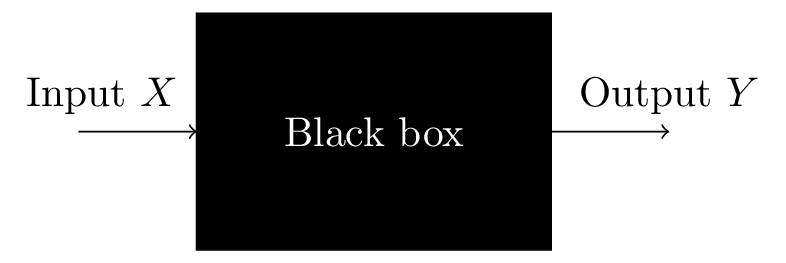
\includegraphics[width=0.5\linewidth]{img/img-ch1/black_box.png}
    \caption{Machine learning blackbox paradigm whose goal is to reproduce input/output pairs based on prior observations.}
    \label{fig:black_box}
\end{figure}


\section{Supervised learning}
First, we  will present the two fundamental learning problems that are faced in the context of machine learning: supervised and unsupervised. The problem of supervised learning can be described in the following formulation:

\begin{definicion}[Supervised learning problem]
    Let $\mathcal{X}$ be an input domain, $\mathcal{Y}$ be an output domain and $\mathcal{D} = \left\lbrace (x_1,y_1),...,(x_M,y_M)\right\rbrace \subset \mathcal{X} \times \mathcal{Y}$ be a dataset that contains inputs $x_i$ and target outputs $y_i$ sampled from a probability distribution $p(x,y)$. Given a new unclassified input $x \in \mathcal{X}$, guess or predict the corresponding output $y \in \mathcal{Y}$
\end{definicion}

In the context of unsupervised learning discussed here, the data samples lack labels, and the objective is to draw similar samples.

\begin{definicion}[Unsupervised learning problem]
    Let $\mathcal{X}$ be an input domain and $\mathcal{D}=\left\lbrace x_1, ..., x_M\right \rbrace \subset \mathcal{X}$ be a dataset of input samples drawn from a probability distribution $p(x)$. The problem consists on drawing a new sample from $p$. 
\end{definicion}

There are other tasks in unsupervised learning such as clustering and dimensionality reduction.

This thesis will be constrained to the case of supervised learning tasks. The standard procedure in supervised learning can be summarized in the following steps:
\begin{enumerate}
    \item Choose a model family $\left\lbrace f \right\rbrace$, that is, a set of trial functions that map inputs from $\mathcal{X}$ to outputs from $\mathcal{Y}$. They usually depend on a set of parameters $\theta$. Each set $\theta$ defines a particular model in the family $\left\lbrace f_{\theta}\right\rbrace$. Next we will proceed to pick the best model to reproduce the data.

    \item This task is formally known as risk minimisation. This process uses a loss function $L(f(x),y)$ which we can understand as a measure of the discrepancy between the model's prediction $f(x)$ for an input $x\in \mathcal{X}$ and its label $y \in \mathcal{Y}$. 

    \item Once we can compute the loss function, we need to choose an optimization algorithm to minimize the average loss over all the data depending on the parameters. Popular choices are gradient descent and stochastic gradient descent.
\end{enumerate}

The difficulty in machine learning lies in the task of selecting the most suitable model without having access to all the data, but instead only having a finite set of examples. Consequently, the essence of learning lies in choosing a model that generalises well from these limited examples to the entire data domain.

As we can see, the model, the data and the learning procedure (which corresponds to the last two steps) are the main components of supervised learning.

\subsection{Data}
Data is the starting point of machine learning and its fuel. The dataset of a supervised learning problem  ${\mathcal{D} = \left\lbrace (x_1,y_1),...,(x_M,y_M)\right\rbrace \subset \mathcal{X} \times \mathcal{Y}}$ is sampled from a joint distribution $p(x,y)$. The set of data samples is taken independently and identically distributed, shortened iid. This is a strong assumption that means that any sample does not depend on the value of the others and has been drawn from exactly the same distribution. This does not really correspond with real life situations but facilitates the learning theory built upon it. Learning in non-iid scenarios remains an open research question. 

We are abstractly talking about data, although what it really is? A \textbf{dataset} is a collection of \textbf{data samples}. Each data sample is a description of an event, an object or the item in question. This description is a collection of \textbf{attributes} or features and their values, which can be qualitative or quantitative, are called \textbf{attribute values}. \autoref{fig:example_dataset} depicts an example of a dataset.

Let ${\mathcal{D} = \left\lbrace (x_1,y_1),...,(x_M,y_M)\right\rbrace \subset \mathcal{X} \times \mathcal{Y}}$ be a dataset containing $M$ samples: $x_i \in \mathcal{X}$ and its corresponding label $y_i \in \mathcal{Y}$. Each data sample $x_i = (x_{i1},..., x_{iK}) \in \mathcal{X}$ is a vector of attributes in the $K$-dimensional input space $\mathcal{X}$ and $x_{ij}$ is the value of the $j$th attribute of the sample $x_i$. Regarding the output space, it determines an important distinction in the type of supervised learning problem to be solved. If $\mathcal{Y}$  is a set of discrete class labels $\left \lbrace l_1, ... l_R \right\rbrace$, we are dealing with a \textbf{classification} problem. In the particular case of $\mathcal{Y} = \left\lbrace l_1, l_2 \right\rbrace$ consits on two labels, then it is called a \textbf{binary classification} problem. If the output space is continuous, such as the space of real numbers $\mathbb{R}$ or an interval therein, then it is a \textbf{regression} problem, that is, the prediction is continuous-valued.

\begin{figure}
    \centering
    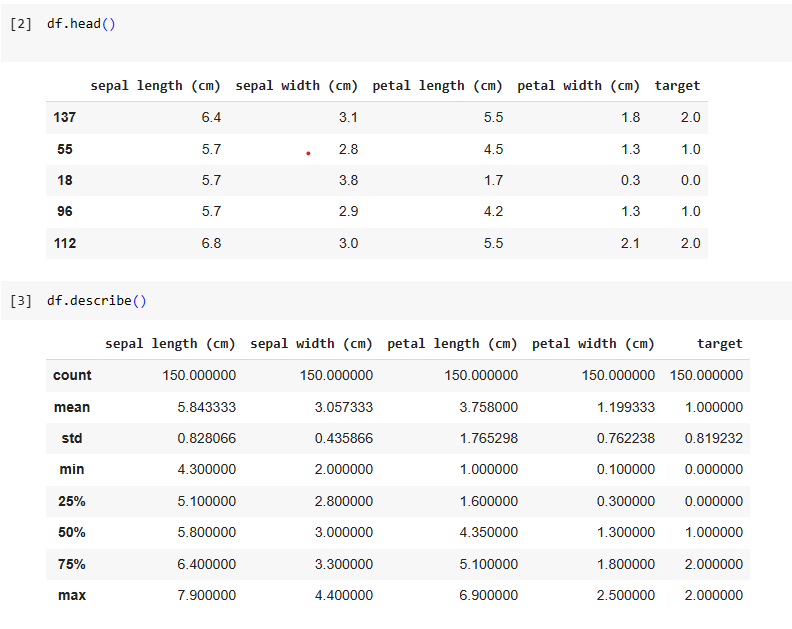
\includegraphics[width=0.8\linewidth]{img/img-ch1/iris_dataset.png}
    \caption{Example of a dataset. It corresponds to the scikit-learn Iris Dataset.\\ This data sets consists of 3 different types of irises’ (Setosa, Versicolour, and Virginica) thus, define a three label classification problem. \\
    There are four attributes: petal and sepal length and width.}
    \label{fig:example_dataset}
\end{figure}


It is desirable to have a data input space $\mathcal{X}$ in $\mathbb{R}^K$, but sometimes raw data is not from a numerical domain and it is needed to first find a suitable quantitative representation of the attributes. There are different techniques depending on the type of data, such as text or images. We cannot go into greater depth because it is a field beyond the scope of this thesis. 

There is vital step for any machine learning application: \textbf{data pre-processing}. This practice impacts the output of the machine learning algorithm and thus, improves its predictive power. Real world data is usually incomplete, dirty and inconsistent, hence data preprocessing techniques are needed to improve the accuracy and efficiency of the machine learning model used. Dirty data include missing data and wrong noisy data . The presence of a high proportion of the data is dirty, implies that the outcome of applying a machine learning algorithm will likely result in an unreliable model. So first, the data must be cleaned to remove or repair dirty data. Then, a series of data transformations are performed because the data collected in a dataset may not be useful enough, that is, the original attributes may have a meaning in its domain but are not convenient to obtain accurate predictions. There are a series of available transformations to change the original attributes or to generate new attributes with better properties. We can point out data normalization, polynomial transformations, one-hot-enconding (to transform categorical data), dimensionality reduction techniques, among others. For a more in-depth exploration of this topic, we would recommend consulting the book \cite{garcia2015data}, which provides comprehensive coverage and valuable insights on the subject of data pre-processing.

Finally, we have to mention the routinary division of the dataset into three subsets called: training, validation and test. The process of ``learning'' of the ML algorithm is also well-known as training. As we have mentioned before, learning is equivalent to generalising well. The training set is used to minimise the cost function (the average of the loss values coming from all data samples). The validation set is used to estimate the performance after training in order to adapt hyperparameters of the algorithm. The model is implicitly fitted to the validation set because we discard those models that did not perform well on this data. Once the model is fully specified, the test set is used for the final evaluation of the model's generalization ability to provide an unbiased evaluation of the final model. The separation of data into these three partitions is really important for obtaining a good model: one that can generalize well to unseen instances, avoiding overfitting. 


\subsection{Model}

The second main component of machine learning is a model, or precisely, a model family. The goal is to obtain a model that fits the data and produces reliable outputs. In mathematics, a model is a map from an input space $\mathcal{X}$ to an output space $\mathcal{Y}$, in other words, a function that reproduces the pattern in the data.
$$\mathcal{X} \longrightarrow \mathcal{Y}$$
In the context of computation, this mapping is achieved through an algorithm. At a higher level of abstraction, a model sets the hypothesis or rules that leads from input to output. Therefore, models in machine learning are functions, algorithms or rules that establish a connection between input data and output, depending on the point of view we fix. We will continue with the mathematical formulation:

\begin{definicion}[Deterministic model]
    Let $\mathcal{X}$ be an input domain and $\mathcal{Y}$ an output domain for a supervised machine learning problem. We define a deterministic model as a function 
    \begin{equation}
        f: \mathcal{X} \longrightarrow \mathcal{Y}, \quad f(x) = y,\quad x\in \mathcal{X},\, y \in \mathcal{Y}
    \end{equation}
\end{definicion}

Usually, this model depends on a set of parameters $\theta$ and hence defines a model family $\left\lbrace f_{\theta} \right\rbrace$

Depending on the output domain $\mathcal{Y}$ we can distinguish between deterministic models for regression and classification tasks.

Theoretically, machine learning methods could use any possible mapping function $$f: \mathcal{X} \longrightarrow \mathcal{Y}$$ to make predictions of a label $y\in \mathcal{Y}$ by computing $\hat{y}=f(x)$. The collection of all possible maps from the input space to the output domain is denoted by $\mathcal{Y}^{\mathcal{X}}$. To obtain the best model that fits our data, we have to search over this set $\mathcal{Y}^{\mathcal{X}}$. However, it is usually far too extensive for practical machine learning methods to fully explore it. As an example, if we consider a regression problem with dataset in which every sample is only characterized by an real-valued attribute and a real-valued label, then $\mathcal{Y}^{\mathcal{X}}$ would be the collection of all real functions of real variable. Instead, the problem would get simplified if we search for the best model in a subset of the real functions of real variable such as linear functions. In that case we are tackling a regression problem with a linear regression algorithm. In general, practical machine learning methods search and evaluate only a small subset of all possible maps $\mathcal{Y}^{\mathcal{X}}$. This subset of computationally feasible maps is what we referred as model family (denoted before as $\left\lbrace f \right \rbrace$, also called hypothesis space $\mathcal{H}$. The selection of a model family for a machine learning problem is a design choice which involves a tradeoff between computational complexity and the statistical properties of the resulting machine learning method.  This choice takes into account the computational resources at the disposal of a machine learning method. Different computational infrastructures tend to align with different hypothesis spaces. For instance, deep learning methods deployed in a cloud computing environment typically use much larger hypothesis spaces derived from deep neural networks. While deep learning methods would be an overkill for a small embedded system, which would perform much better with a linear hypothesis space. 

In a general sense, the design choice regarding the model family of a machine learning method has two main demands to be balanced: 
\begin{itemize}
    \item The model family as to be sufficiently large so that it contains at least one accurate predictor map $\hat{f}\in \left\lbrace f \right\rbrace$. If the model family is too small, it may not encompass a predictive mapping necessary to capture the (potentially complex and nonlinear) relationship between inputs and outputs.

    \item It has to be sufficiently small such that its processing fits the available computational resources including memory, bandwidth and processing time. At the same time, we must be able to search efficiently to find a good model. Constraining the size of the hypothesis space is also related to the prevention of overfitting since in a large model family we might, by chance, stumble upon a function that almost perfectly predicts the labels of the training set while showing poor generalization power for other data.
\end{itemize}


\subsection{Learning procedure}

A machine learning method has to select the best model from the model family of all computationally feasible predictor maps. This raises the question: which model is the best model out all the possible ones? We need a measure of quality of a model, that is, how close are the model predictions to the target labels. There is where the concept of \textbf{loss function} appears. 

\begin{definicion}[Loss function]
    A loss function is a map
    \begin{align}
        L: \mathcal{X} \times \mathcal{Y} \times \mathcal{H} &\longrightarrow \mathbb{R}^{+} \\
        ((x,y),f) &\longmapsto L(f(x),y)
    \end{align}
    which assigns a pair consisting of a input $x \in \mathcal{X}$, its label $y\in \mathcal{Y}$ and a model $f$ to the non-negative real value $L(f(x),y)$ named loss value.
\end{definicion}

The loss value $L(f(x),y)$ measures the difference between the true label $y $ and the prediction by the model $f(x)$. Now that we have formulated this concept, we can rephrase the basic procedure of machine learning to find a model out of all the model family that minimizes the loss $L(f(x),y)$ for all data inputs.

The loss function is another design choice for the machine learning technique. This decision should take into account the computational complexity for finding a minimum loss (benefiting differentiable and convex functions), robustness to outliers, statistical aspects and interpretability. There exist numerous loss functions, and perhaps the simplest one for classification tasks relies on a model's accuracy, which measures the proportion of correctly classified examples:
\begin{equation}
    \text{accuracy} = \frac{\text{number of samples classified correctly}}{\text{total number of samples}}
\end{equation}
The corresponding loss would be the error:
$$\text{error} = 1-\text{accuracy}$$

Most machine learning methods use a continuous-valued loss function, since differentiability is desirable to compute gradients. One of the most popular loss functions is the norm in $l_2$ or squared Euclidean distance which is known as \textbf{mean-squared-error loss}
$$L(f(x),y)=(f(x)-y)^2$$
The norm in $l_1$ also provides us another loss function:
$$L(f(x),y)=|f(x)-y|$$
Other options are the \textit{hinge loss}
$$L(f(x),y) = \max (0, 1-yf(x))$$
and the \textit{logistic loss}
$$L(f(x),y) =\log (1+e^{yf(x)})$$

The loss function is the starting point of the \textbf{risk minimisation} process that consists on minimising the expected or average loss (called risk ) of a model over the data distribution.
\begin{definicion}[Risk]
    Let the inputs $x \in \mathcal{X}$ and outputs $y \in \mathcal{Y}$ to a supervised learning problem be sampled from a distribution $p(x,y)$. The \textbf{expected loss} or \textbf{risk} of a model $f$ with loss $L$ is defined as
    \begin{equation}
        \mathcal{R}_f = \mathbb{E}[L_f] = \int_{\mathcal{X}\times \mathcal{Y}} L(f(x),y) p(x,y) dx\, dy
    \end{equation}
    Note that the integral runs over all possible data pairs and thus, the expectation is taken over the data distribution.
\end{definicion}

The risk provides an indication of the model's performance across the entire data domain, with a lower risk indicating better performance. The goal to solve a supervised learning problem will be to minimise the risk, although the integral over all possible data pairs is impossible to compute in practice, so we need to estimate the risk over the $M$ data samples we are provided in a dataset. This estimation is called \textbf{empirical risk}.
\begin{definicion}[Empirical risk]
    Consider the dataset ${\mathcal{D} = \left\lbrace (x_1,y_1),...,(x_M,y_M)\right\rbrace \subset \mathcal{X} \times \mathcal{Y}}$. The empirical risk estimates the risk over the dataset as the average loss:
    \begin{equation}
        \hat{\mathcal{R}}_f = \hat{\mathbb{E}}[L_f] = \frac{1}{M}\sum_{i=1}^M L(f(x_i), y_i)
    \end{equation}
\end{definicion}

This estimation is warranted because of the law of large numbers, departing from the assumption that we consider the dataset to be independent and identically distributed variables from the distribution $p(x,y)$. Therefore, the sample average converges to the expected value if the number of samples $M$ of the dataset $\mathcal{D}$ is sufficiently large. 

In practice, we select a model out of the model family minimising the empirical risk on the given dataset, that is, finding the model $f^*$ such that $$f^* = \min_{f \in \mathcal{H}} \hat{\mathcal{R}}_f$$
In parametrised model families, model selection translates to optimising the parameters. Therefore, the empirical risk minimisation can be reformulated as finding the parameter $\theta^*$ such that
$$\theta^*=\min_{\theta} \hat{\mathcal{R}}_{f_{\theta}}$$

Machine learning should solve the empirical risk minimisation problem without overfitting: there is an optimal solution of the empirical risk over the training data that performs poorly on new data. There are different strategies to prevent the model from overfitting: \textbf{regularisation techniques}. The most common one is to add a regularisation term $g(f_{\theta})$ to the empirical risk and minimise the cost function
$$C(\theta)=\hat{\mathcal{R}}_{f_{\theta}} + g(f_{\theta})$$
These regularisation terms penalize the model and impose additional constraints, for example the $l_1$ regulariser
$$g_{l_1}(\theta)=\sum_{i}|\theta_i|$$
benefits parameters with a small absolute value, while the $l_2$ regularisation term
$$g_{l_2}(\theta)=\sum_i \theta_i^2$$
adds preference to parameters with a small $l_2$ norm.

Once we have formulated the cost function, the learning procedure consists on an optimisation problem. While there is an extensive theory and algorithms for convex optimisation problems,  machine learning tasks usually fall into non-convex optimisation problems for which there is significantly less information available. The popular choice to tackle this sort of non-convex optimisation are iterative searches that progressively calculate better candidates for the parameters of a model.
In situations where there are multiple parameters and optimization occurs within high-dimensional spaces, we need to understand the landscape of the cost function. The main source of information in such cases is gradients: a vector of partial derivatives of a function with respect to its inputs. The gradient provides the direction of the most significant incline in the cost landscape.

\textbf{Gradient descent} is an iterative algorithm for finding the minimum of a differentiable function. The general idea of this algorithm is to update the parameters $\theta$ of a cost function $C(\theta)$ iteratively towards the direction of steepest descent in order to minimize a cost function. We can think of this situation in a real world scenario: suppose you are lost in the mountains blindfolded, you can only feel the slope of the ground below your feet. Your goal is to reach to the lowest point going downhill in the direction of the steepest slope. 

This is mathematically expressed as
$$\theta_{t+1} = \theta_{t}-\eta\nabla C(\theta_t)$$
where $\eta$ is a parameter called learning rate that determines the step size at each iteration and $t$ is an integer that corresponds to the current iteration. \autoref{fig:gradient_descent} illustrates this algorithm for a really simple scenario.

If the learning rate is too small, the algorithm will have to perform many iterations to converge. Whereas if the learning rate is too high, you might jump across the valley and end up on the other side, perhaps even at a higher point than in the previous step and eventually the algorithm may diverge. This situations are depicted in \autoref{fig:learning_rates}.

\begin{figure}
    \centering
    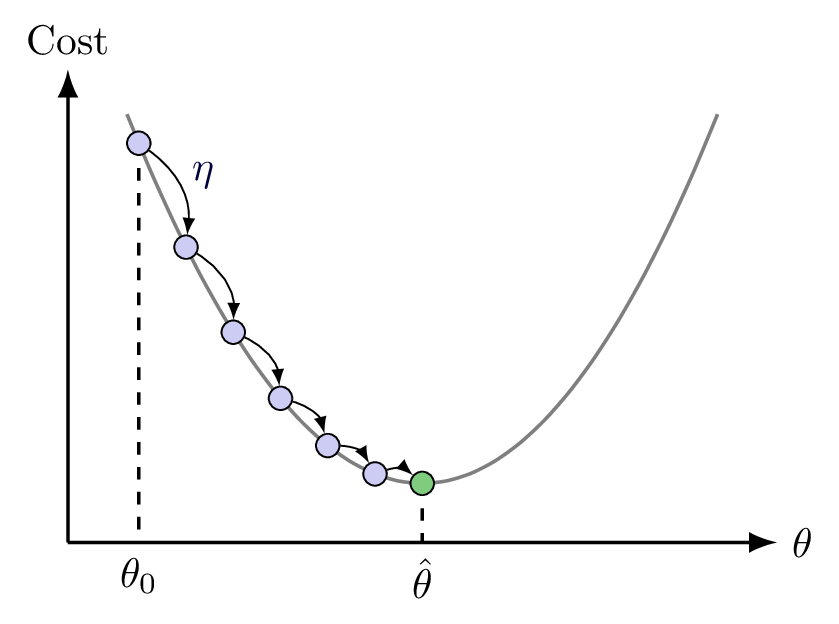
\includegraphics[width=0.6\linewidth]{img/img-ch1/gd.png}
    \caption{Gradient descent}
    \label{fig:gradient_descent}
\end{figure}

\begin{figure}
    \centering
    \begin{subfigure}{0.5\textwidth}
        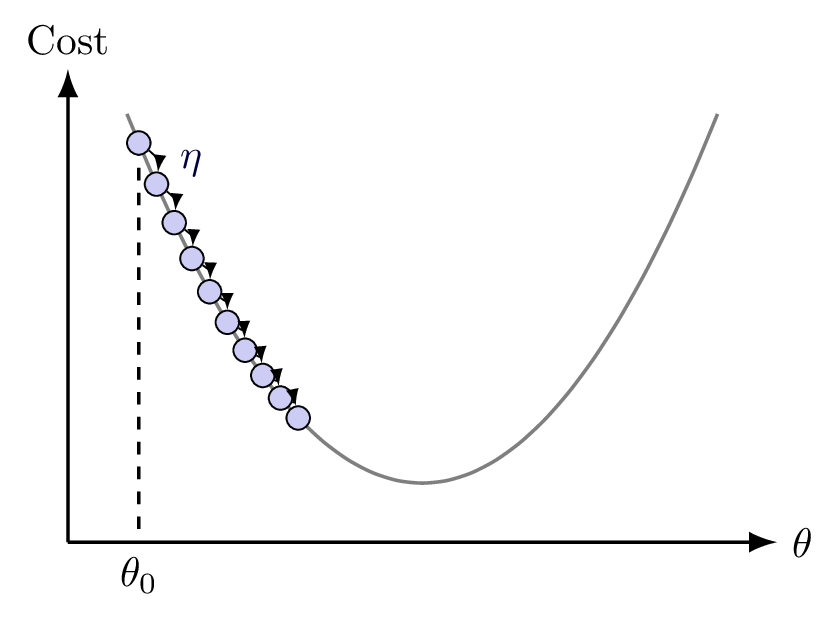
\includegraphics[width=\linewidth, keepaspectratio]{img/img-ch1/gd_small.png} 
        \caption{Gradient descent algorithm taking a $\eta$ learning rate too small}
        \label{fig:GD small learning rate}
    \end{subfigure}
    
    \begin{subfigure}{0.5\textwidth}
        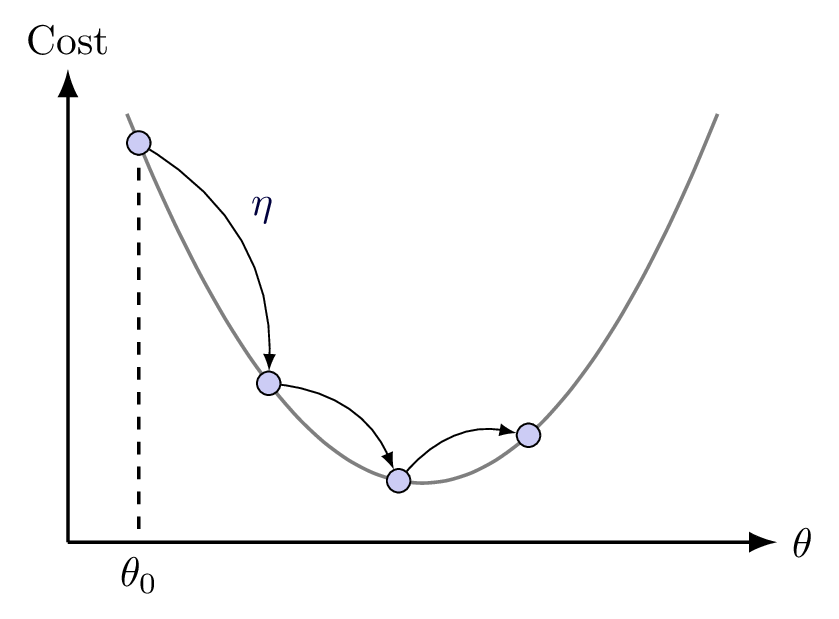
\includegraphics[width=\linewidth, keepaspectratio]{img/img-ch1/gd_big.png}
        \caption{Too big $\eta$ learning rate for gradient descent}
        \label{fig:GD big learning rate}
    \end{subfigure}
    
    \caption{Effect of different learning rates for gradient descent algorithm}
    \label{fig:learning_rates}
\end{figure}

The formula above of the gradient descent algorithm performs the purpose of the process: the gradient $\nabla C(\theta_t)$ always points towards the ascending direction in the landscape of the cost function $C$, thus $- \nabla C(\theta_t)$ points to the opposite direction, that is, the descending direction. The initial set of parameters $\theta_0$ is randomly initialized. Then, it is gradually improved, at each step attempting to decrease the cost function. 

In real case scenarios, cost functions may differ very much from the previous illustrations. There may be holes, plateaus, ridges and all sorts of irregular terrains, making convergence to the minimum very difficult.

There are several variations of the gradient descent algorithm such as batch gradient descent, stochastic gradient descent and mini-batch gradient descent. \cite{geron2022hands}

\subsection{Evaluation metrics}
After training and finding a model that performs sufficiently well, it is time to evaluate the final model on the test set. First, we need to apply the model to the test set to obtain the predictions. Then, having the predictions and the labels we can apply different metrics to evaluate the performance of the model.

There are many performance measures available. In the context of classification, we will consider the following ones:

\begin{itemize}
    \item \textbf{Accuracy.} This metric represents the ratio of correct predictions to the total number of samples.
    \begin{equation}
        \text{accuracy} = \frac{\text{number of samples classified correctly}}{\text{total number of samples}}
    \end{equation}

    It gives us a general idea of the classification power of our model, although we have to take into account that it is not a good metric in the case of a dataset with unbalanced classes since it is ``blind'' to different classes. To understand it, let's consider a dataset with 100 samples, 97 of them are labeled 0 and 3 correspond to label 1. If our model predicts label 0 for all samples, the accuracy would be of 97\% which does not represent the actual lack of classification power of the model. 
    
    \item \textbf{Confusion matrix.} 
    A confusion matrix is a table used to evaluate the performance of an algorithm. Each row corresponds to a label and each column represents a predicted label. Therefore, if $n$ is the number of labels of the dataset, the confusion matrix is a $n \times n$ table that shows the correct and incorrect predictions made by the model compared with the actual labels.

    In the case of a binary classification problem we have the following confusion matrix, considering \textit{P} is the number of positive labels (1) and \textit{N} is the number of negative labels (0). 

    
    
    \begin{table}
        \centering
        \setlength{\tabcolsep}{10pt} % Default value: 6pt
        \renewcommand{\arraystretch}{1.5} % Default value: 1
        \begin{tabular}{|c|cc|}
            \hline
             & PP  & PN \\
             \hline
            P & TP & FN\\
            N & FP & TN\\
            \hline
        \end{tabular}
        \caption{Confusion matrix of a binary classification problem.}
        \label{tab:confussion_matrix}
    \end{table}
    In figure \autoref{tab:confussion_matrix}, TP stands for true positive, FP - false positive, TN - true negative and FN - false negative. These values are used to compute other metrics.
    
    \item \textbf{Precision.} It is the ability of a model not to label as positive a sample that is negative. 
    \begin{equation}
        \text{Precision} = \frac{TP}{TP + FP}
    \end{equation}
    It is useful for unbalanced datesets, since the precision is inversely proportional to the number of false positives.
    
    \item \textbf{Recall.} It is the ability of the classifier to find all the positive samples.
    \begin{equation}
        \text{Recall} = \frac{TP}{TP + FN}
    \end{equation}
    
    \item \textbf{$F_1$ score.} It can be interpreted as the harmonic mean of the precision and recall. 
    \begin{equation}
        F_1 = \frac{2 \cdot \text{precision} \cdot \text{recall}}{\text{precision} + \text{recall}} = \frac{2 TP}{2 TP + FP + FN}
    \end{equation}
    This metrics takes values in the interval $\interval{0}{1}$. The higher $F_1$, the better is the performance of the model.
    
    
    \item \textbf{ROC curve.} It stands for Receiver operating characteristic curve. It is a graph that shows the performance of a binary classifier as its discrimination threshold (the threshold for deciding whether a prediction is labeled positive or negative) is varied. It represents the tradeoff between the TPR = true positive rate (fraction of true positives out of all the positives) and the FPR = false positive rate (fraction of false positives out of all the negatives). A perfect model would have high value of true positive rate and low value of false positive rate.

    \item \textbf{AUC.} It computes the area under the ROC curve. This metric summarizes the curve information in one number. AUC has a range of [0,1]. The greater the value, the better is the performance of our model.
\end{itemize}


Up to this point, we have observed that the objective in machine learning is to choose a model that reduces a specific cost function which depends on data samples of a particular task, with the ultimate goal of minimizing the cost when applied to unseen data. If the model is parametrised, the selection process involves optimizing or "training" these parameters minimise the cost. 

There are many methods in machine learning, that is, model function families that can be used for prediction and a training strategy for how to use the data to construct a specific model that generalises from it. In the following sections, we will introduce two classical machine learning methods: support vector machines and neural networks, that will become important in the context of quantum machine learning in the following chapters. 


\section{Support vector machines}

 Support vector machine (SVM) is a supervised learning algorithm for binary classification. In particular, SVM are one of the most well-known kernel methods. Kernel methods work out machine learning problems based on the concept of measuring similarity between data points. This similarity measure is expressed by a \textbf{kernel}.
 

 \subsection{Kernel methods}\label{subs:kernel-methods}
 \begin{definicion}[Kernel]
     Given a data domain $\mathcal{X}$, a kernel is a positive semi-definite bivariate function $\kappa : \mathcal{X} \times \mathcal{X} \longrightarrow \mathbb{R}. $ 
 \end{definicion}
 
 Mercer's theorem provides the following useful characterization of kernels.
 \begin{teorema}
     The function $\kappa: \mathcal{X} \times \mathcal{X} \longrightarrow \mathbb{R}$ is a Mercer kernel function (also known as kernel function) where:
     \begin{enumerate}
         \item it is symmetric: $\kappa (x,y) = \kappa(y,x), \, \forall x,y \in \mathcal{X}$,
         \item its kernel matrix, that is, the kernel applied on a set of data points of the input space $\mathcal{D}=\left \lbrace x_1,...,x_M\right\rbrace $ forms a $M \times M$ Gram matrix: $\mathcal{K}(i,j)=\kappa(x_i, x_j), \quad \forall i,j \in \left\lbrace1,...,n\right\rbrace$ is positive semi-definite.
     \end{enumerate}     
 \end{teorema}

 
 A great part of the theory of kernel methods relies on \textbf{``the kernel trick''}: the fact that kernel functions can be represented as inner products of data that has been mapped from its original space $\mathbb{R}^n$ into a higher dimensional space $\mathbb{R}^N$ ($n<N$), in which machine learning algorithms can solve problems by the use of inner product. This higher dimensional space receives the name of feature space $\mathcal{F}$. The potential of this idea is that in a suitable feature space we would obtain linearly separable data by a hyperplane. The function that takes original data inputs into the feature space is called \textbf{feature map} $\phi : \mathcal{X} \longrightarrow \mathcal{F} $.

 Thus, we just need to compute: 
 \begin{equation}
     \kappa(x, y) = \left< \phi(x), \phi(y) \right>_{\mathcal{F}}
 \end{equation}

 In turn, a model is expressed in terms of a kernel function. We obtain different models by replacing the kernel functions. 

Support vector machine provides a decision boundary (a hyperplane in the feature space) separating the considered classes such that its distance to each class is as large as possible. This idea derives from their initial introduction as maximum-margin classifiers, which advocates that during training, the goal is to maximize the separation between the decision boundary of a classifier and the training data points.

An introduction to maximum-margin classifiers will help us to understand better the working principle of support vector machines.

Let's consider a binary classification problem with an input domain $\mathcal{X} = \mathbb{R}^n$ and output domain $\mathcal{Y}=\left\lbrace -1, 1\right\rbrace$. 

We assume that our data is linearly separable by a hyperplane, which means that there is a normal vector $\vec{w} \in \mathbb{R}^n$ and some constants $b \in \mathbb{R}$ which define a hyperplane $\vec{w}\cdot \vec{x} +b =0$ that separates the training data so that points of the two different classes are on either side of the hyperplane. We will denote this hyperplane as $H$. We can determine to which side of the hyperplane our data $x \in \mathcal{X}$ is in terms of the sign of $\vec{w}\cdot \vec{x} +b$. 

We take a linear model as this hyperplane and simplify the vectorial notation
$$f_{w}(x) = w^T x + b$$

Linear separation can be expressed by the restriction $f_w(x_i) >0$ for data points labeled $y_i = 1$, and $f_w(x_i)<0$ for inputs of class $y_i=-1$. According to this, linear separation can be summarised in the following condition 
$$f_w(x_i)y_i > 0 \quad \forall i=1,...,M$$

There are infinite number of separating hyperplanes, but we are looking for the one that would maximize the distance to the training datapoints and therefore, obtain a classifier with a low risk because we expect unseen data to follow a similar distribution to the one that we have seen in the training data, that is, new samples of one class will be close to training samples of that class. Support vector machine looks for the separating hyperplane that maximises the distance between the closest training points and itself. This distance is known as \textit{margin}.

Let's consider $p_0$ the closest data point to $H$ and consider the hyperplane parallel to $H$ that contains $p_0$. This hyperplane and its reflection define the margin of $H$ and can be represented by the equations $\vec{w}\cdot \vec{x} +b =\pm C$ for some constant $C$. We can divide the expression by $C$ to obtain the margin hyperplanes: $$\hat{w} \vec{x} + \hat{b} = \pm 1$$
where $\hat{w}=\vec{w}/C$ and $\hat{b}=b/C$.

The separating hyperplane $H$ can be represented by $$\hat{w} \vec{x} + \hat{b} = 0$$
We will denote the margin hyperplanes as $H_1$ and $H_{-1}$ accordingly.

We are working under the assumption that there are no points inside the margin. Studying the sign of $\hat{w} \vec{x_0} + \hat{b}$ for $x_0 \in \mathbb{R}^n$ we can determine to which region it belongs:
\begin{itemize}
    \item If $\hat{w} \vec{x_0} + \hat{b} = 0$, then $x_0$ is in the hyperplane $H$.
    \item If $0<\hat{w} \vec{x_0} + \hat{b}<1$, then $x_0$ is in the margin between the hyperplanes $H$ and $H_1$.
    \item If $-1<\hat{w} \vec{x_0} + \hat{b}<0$, then $x_0$ is in the margin between the hyperplanes $H$ and $H_{-1}$.
    \item If $\hat{w} \vec{x} + \hat{b} = \pm 1$, then $x_0$ is in one the hyperplanes that defines the margin, $H_1$ or $H_{-1} $ respectively.
\end{itemize}

The condition of linear separation with margin can be expressed with the constraint:
$$f_w(x_i)y_i>1 \quad \forall i=1,...,M$$

Let's remember that our goal is to maximize the margin while preserving the condition of linear separation with margin that we have derived above. Now we will deduce what is the expression of the margin, which is the distance between the hyperplanes $H_1$ and $H_{-1}$. 

First we will see what is the distance between $H$ and $H_1$: the length of the only vector in the direction normal to $H_0$ that connects $p \in H_0$ to a point in $H_1$. Since $\hat{w}$ is normal to $H_0$, the desired vector needs to be $\alpha \hat{w}$ for some scalar $\alpha$. Therefore, $p + \alpha \hat{w} \in H_1$ and it must fulfill its equation:
\begin{align}
    \hat{w}(p+\alpha \hat{w}) +b &= 1 \\
    \hat{w}p + b + \alpha ||\hat{w}||^2 &= 1
\end{align}
Since $p \in H_0$, we have that $\hat{w}p + b =0$. We can obtain the scalar $\alpha$ from the expression above
$$\alpha ||\hat{w}||^2=1 \Longleftrightarrow \alpha = \frac{1}{||\hat{w}||^2} $$

The length of $\alpha \hat{w}$ would be $$||\alpha \hat{w}|| = |\alpha| \cdot ||\hat{w}|| = \frac{1}{||\hat{w}||^2} ||\hat{w}|| = \frac{1}{||\hat{w}||}$$

Therefore, the distance between $H_1$ and $H_{-1}$ is by symmetry the double of the distance between $H$ and $H_1$, that is $\frac{2}{||\hat{w}||}$. 

The problem of finding a hyperplane that separating the data maximizes the margin can be posed as the following optimization problem
\begin{align}
    \text{Maximize: \quad } &\frac{2}{||\hat{w}||} \\
    \text{subject to: \quad } &f_w(x_i)y_i>1 \quad \forall i=1,...,M
\end{align}

The above optimisation problem of finding the maximum margin becomes equivalent to the next minimization problem
\begin{align}
    \text{Minimize: \quad } &||\hat{w}|| \\
    \text{subject to: \quad } &f_w(x_i)y_i>1 \quad \forall i=1,...,M
\end{align}

Alternatively, it is possible to minimise $\frac{1}{2} ||\hat{w}||^2$ under the same constraint, leading to the same solution but easier to solve. Now we are going to briefly present the dual SVM problem which is equivalent to 
\begin{align}
    \text{Minimize: \quad } &\frac{1}{2}||\hat{w}||^2 \\
    \text{subject to: \quad } &f_w(x_i)y_i>1 \quad \forall i=1,...,M
\end{align}
This is a quadratic optimization problem with $n+1$ variables ($\hat{w}\in\mathbb{R}^n$ and $b\in \mathbb{R}$) and $M$ constraints. It is computationally difficult to solve when $n$ is large. The dual problem will also be a quadratic optimization problem but with $M$ variables and $M+1$ constraints. The solution gives us the same optimal hyperplane but the dual problem is often easier and it also allows us to exploit the kernel trick that we mentioned before. 

The first task is to construct the Lagrangian. The optimization variables are $b$ and $w$. There are $M$ constraints, so we introduce $M$ penalty terms and a Lagrange multiplier $\alpha_m$ for each of them. The Lagrangian is:
\begin{align}
    \mathcal{L}(b,w,\alpha) &= \frac{1}{2}w^2 +\sum_{m=1}^M \alpha_m(1- y_m(w^T x_m +b)) \\
    &= \frac{1}{2}w^2 - \sum_{m=1}^M \alpha_m y_m w^T x_m - b \sum_{m=1}^M \alpha_m y_m + \sum_{m=1}^M \alpha_m
\end{align}
First, we have to minimize $\mathcal{L}$ with respect to $b$ and $w$. We obtain its partial derivatives:
\begin{itemize}
    \item The partial derivative with respect to $b$ is the coefficient of $b$ because it appears linearly in the Lagrangian. $$\frac{\partial \mathcal{L}}{\partial b} = -\sum_{m=1}^M \alpha_m y_m$$
    \item Using some linear algebra identities, we can obtain that the gradient with respect to $w$ is 
    $$\frac{\partial \mathcal{L}}{\partial w} = w - \sum_{m=1}^M \alpha_m y_m x_m$$
\end{itemize}

We can derive the dual form by noting that the gradient of $\mathcal{L}$ with respect to $w$ is zero if 
$$w = \sum_{m=1}^M \alpha_m y_m x_m$$
On the other hand, the partial derivative with respect to $b$ is zero if $$\sum_{m=1}^M \alpha_m y_m = 0$$

Therefore, 
$$\mathcal{L}(b,w,\alpha) = \frac{1}{2}w^2 - \sum_{m=1}^M \alpha_m y_m w^T x_m  + \sum_{m=1}^M \alpha_m$$

We can substitute $w = \sum_{m=1}^M \alpha_m y_m x_m $ in the first two terms of the sum. After groping and operating we would obtain the final expression of the Lagrangian that only depends on $\alpha$
\begin{equation}
    \mathcal{L} = \sum_{m=1}^M \alpha_m - \frac{1}{2} \sum_{m,n = 1}^M y_m y_n \alpha_m \alpha_n x_m^T x_n
\end{equation}
This is know as the dual Lagrangian function. It describes a convex optimisation problem with $M$ variables, where $M$ is the number of training samples.

Once obtained this formulation, the optimisation problem is translated into an equivalent minimization task:
\begin{align}
    \text{Minimize: \quad } &\sum_{m=1}^M \alpha_m - \frac{1}{2} \sum_{m,n = 1}^M y_m y_n \alpha_m \alpha_n x_m^T x_n \\
    \text{subject to: \quad } &\sum_{m=1}^M \alpha_m y_m = 0 \\
    &\alpha_m \geq 0 \quad m=1,...,M
\end{align}

Once the optimal Lagrangian multipliers $\alpha^*$ are found, we are just missing to compute the optimal hyperplane. The optimal weights $w_*$ are obtained from the condition 
$$w_* = \sum_{m=1}^M \alpha_m^* y_m x_m$$

We can compute predictions with the linear model 
$$f_{w_*}(x) = w_*^T x + b$$
or in the dual space
$$f(x) = \sum_{m=1}^M \alpha_m^* y_m x_m^T x +b$$

It is worth noting that the dual Lagrangian optimisation expression and the model in the dual space above rely only on the inner product $\braket{x_i,x_j }$ between data samples $x_i, x_j$. We can replace this inner product with an inner product in a feature space $\mathcal{F}$ and there is where kernels appear: $\kappa(x_i,x_j)=\braket{\Phi(x_i),\Phi(x_j)}_{\mathcal{F}}$ 

This way, the linear model is turned into a linear model in the feature space:
$$f_w(x) = \braket{w, \Phi(x)}_{\mathcal{F}} + b$$
with $w \in \mathcal{F}$.

The initial condition of linear separability of the data is translated to a feature space of higher dimension. Nonlinear data can be linearly separable in a feature space where the maximum-margin classifier becomes a kernel method that can candle non separable data. This way, SVM can find nonlinear decision boundaries in input space. 


\section{Neural networks}

Artificial neural networks are a fundamental component of artificial intelligence, that has revolutionized the field of machine learning and continue to drive innovation in various domains. These computational models were born taking the brain's architecture as inspiration. The human nervous system contains cells, which receive the name of neurons. They are composed of a cell body called ``soma'' containing the nucleus and most of the cell's complex components, and many branching extensions called ``dendrites'' plus one long extension called the ``axon''. At the tip of the ramifications of the axon there are tiny structures called ``synaptic terminals'', or simply ``synapses'', which are connected to the dendrites of other neurons. \autoref{fig:bio-neuron} is an illustration of a neuron and its parts.

Biological neurons receive signals, short electrical impulses from other neurons through the synapses. A neuron fires its own signals once the incoming signal surpasses a certain threshold value. This is know as the \textbf{integrate and fire} principle, one of the simplest models of a neuron’s electrical properties and probably the most commonly used in the field of neuroscience. The strengths of synaptic connections often change in response to external stimuli. At first glance, it looks like individual neurons behave in a rather simple way, yet they are organized in a vast network comprising billions of neurons, with each neuron usually connected to thousands of other neurons. The cortex of different species has been observed to display a laminar or layered structure. Each individual layer within the cortex showcases a unique distribution of different types of neurons and their respective connections. The structure of biological neural networks remains a topic of ongoing investigation and research.

\begin{figure}
    \centering
    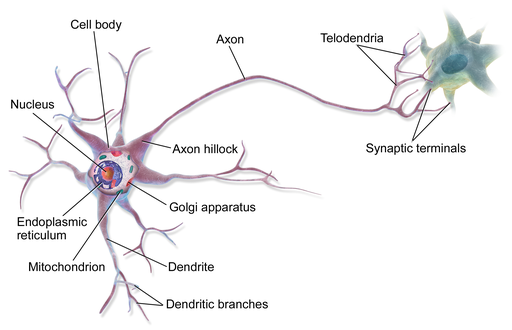
\includegraphics[width=0.7\linewidth]{img/img-ch1/Blausen_0657_MultipolarNeuron.png}
    \caption{Biological neuron. Image by BruceBlaus, \href{https://creativecommons.org/licenses/by/3.0}{CC BY 3.0}, via Wikimedia Commons}
    \label{fig:bio-neuron}
\end{figure}


This biological mechanism is simulated in artificial neural networks. The artificial neurons are the computational units that are connected with each other through weights, which model the strengths of synaptic connections present in the biological case. Every input received by a neuron is scaled by a weight factor, influencing the function computed by that specific unit. An artificial neural network processes the input values by propagating their computed values from the input neurons to the output neuron(s) while leveraging the weights as intermediary parameters, in order to learn. Similar to how biological organisms require external stimuli for learning, artificial neural networks rely on training data containing examples of input-output pairs, which serve as the external stimulus for the learning process. 

Throughout this section, we will use the term neural networks to refer to artificial neural networks, leaving behind the biological ones.

\subsection{Perceptron}
The perceptron is the simplest neural network, proposed in 1957 by Frank Rosenblatt \cite{rosenblatt1958perceptron}. It has a single input layer and an output node. It computes a weighted sum of its inputs $\left\lbrace x_1,...,x_n\right\rbrace$: $z = w_1x_1+...w_nx_n = w^T x$, where $x=(x_1,...,x_n)$ is the input vector and $w = (w_1,...,w_n)$ is the weight vector. Then, applies a non linear function $\varphi$ called the activation function. \autoref{fig:perceptron} displays the graphical representation of a perceptron.

In the original proposal of the perceptron, it was formulated with the Heaviside function, also known as step function, which is applied to that sum. Finally, it outputs the result. The model function of the perceptron is given by
\begin{equation}
    f(x,w)=H(w^T x)
\end{equation}
where $H$ is the Heaviside function (plotted in \autoref{fig:heaviside})
\begin{equation}
    H(x) =
    \begin{cases}
    0 & \text{if } z < 0 \\
    1 & \text{if } z \geq 0
    \end{cases}
\end{equation}

\begin{figure}
    \centering
    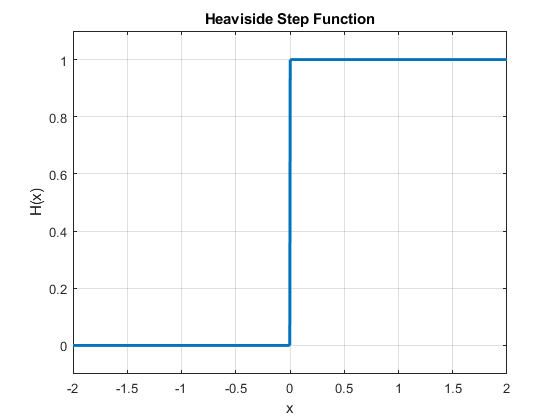
\includegraphics[width=0.7\linewidth]{img/img-ch1/heaviside_graph.png}
    \caption{Plot of the Heaviside step function}
    \label{fig:heaviside}
\end{figure}

\begin{figure}
    \centering
    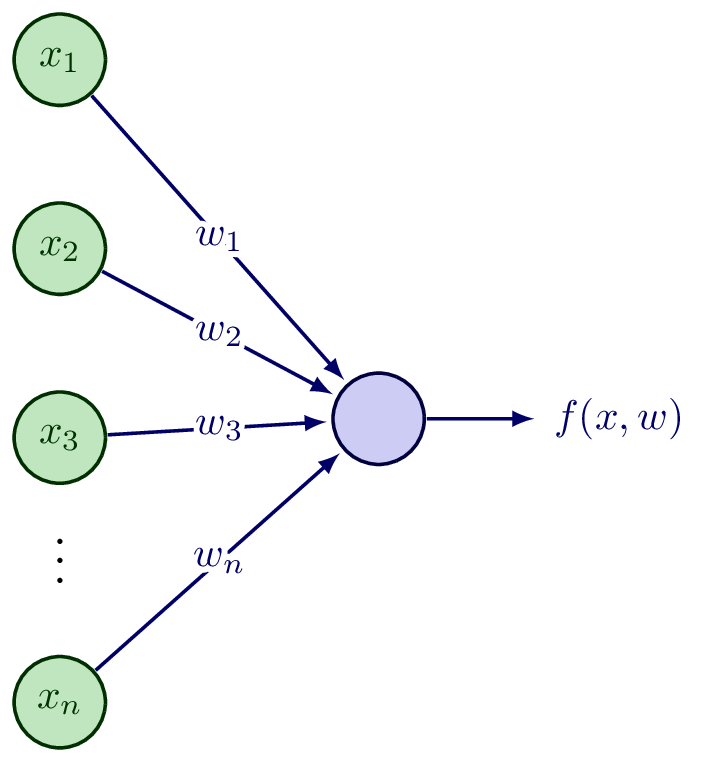
\includegraphics[width=0.5\linewidth]{img/img-ch1/perceptron.png}
    \caption{Illustration of the perceptron model. The inputs are displayed as nodes of graph called \textit{neurons}. Each input unit is linked to the output unit through a weighted connection.}
    \label{fig:perceptron}
\end{figure}


The perceptron can be used for linear binary classification. It computes a linear combination of the inputs and if the result exceeds a threshold, it outputs the positive class, otherwise it outputs the negative class, just like it does a linear support vector machine. 

At the time the perceptron was proposed by Rosenblatt, the parameter optimization was performed in a heuristic way with hardware circuits (\textit{Mark I perceptron}) and it was not presented in terms of a formal notion of optimization in machine learning. The training was inspired by \textit{Hebb's rule}. Donald Hebb suggested in 1949 \cite{hebb2005organization} that when a biological neuron often triggers another neuron, the connection between them two grows stronger. The Hebbian learning is derived from this and states that the connection weight between two neurons is increased whenever they have the same output. Perceptrons are trained taking into account the error made by the network, reinforcing connections that help reduce the error. The training of the perceptron model is done by iterating through the training data and updating the weights according to the following rule
\begin{equation}
    w_{i,j}^{\text{next step}} = w_{i,j} + \eta (y_j - \hat{y}_j) x_i
\end{equation}
\begin{itemize}
    \item $w_{i,j}$ is the connection weight between the $i$-th input neuron and the $j$-th output neuron.
    
    \item $\eta$ is the learning rate.
    
    \item $x_i$ is the $i$-th input value of the current training sample.
    
    \item $y_j$ is the label of the $j$-th output neuron for the current training sample.
    
    \item $\hat{y}_j$ is the output of the $j$-th output neuron for the current training sample. 
\end{itemize}

The perceptron model has several weak points. It is only valid for linearly separable datasets, which excludes learning a simple XOR function. Additionally, the Heaviside activation function is not differentiable.  

\subsection{Feed-forward neural networks}

Neural networks are composed of one \textit{input layer}, one or more layers of perceptrons called  \textit{ hidden layers}, and one \textit{output layer}. In other words, a neural network are stacked perceptrons, hence they are also referred to as multilayer perceptron. The most important neural network structure is the feed-forward neural network, which has an acyclic layering structure of perceptrons so that outputs of one perceptron are the input of another in the following layer.  In the rest of the section we will simply say neural networks when referring to feed-forward neural networks.

The function that expresses neural networks as a deterministic model can be expressed as 
\begin{equation}
    f_{W_1, W_2,..., W_L}(x) = \varphi_L(w_L \varphi_{L-1}(W_{L-1} \cdots \varphi_2(W_2 \varphi_1(W_1 x) ) \cdots ) )
\end{equation}
where $x \in\mathcal{X}$ is an input, $W_i, \, i=1,...,L$ is a real valued matrix of weights of the $i$-th layer and $\varphi_i$ is the activation function in vectorised form, that is, the variable is a vector and the function acts element-wise returning a vector of the same size. 

For many years, researchers encountered challenges to find a way to train neural networks, until the \textbf{backpropagation algorithm} was introduced. In essence, it is simply gradient descent using an efficient technique for computing the gradients automatically in two passes through the network (one forward and one backwards). The backpropagation algorithm is able to compute the gradient of the cost function (the model's generalisation error) with respect to every single model parameter. Once it has these gradients, it performs regular gradient descent. The whole process is repeated until convergence to the optimal solution is obtained. Later, we will come back to this idea in detail.

Previously, we presented the activation function of the perceptron: the Heaviside function. This introduces two problems when working with neural networks:
\begin{enumerate}
    \item The Heaviside function is not differentiable at $x=0$ and has $0$ derivative elsewhere, so there is no gradient to work with since gradient descent cannot progress on a flat surface. 

    \item The goal of a neural network is to learn the values of the weights so that the output from the network correctly classifies the data, therefore, it is desirable to have stability, that is a small change in the weight to cause only a small corresponding change in the output of the network. This way, we can modify the weights little by little towards the behaviour that approximates best the data. The problem is that the output of the Heaviside function is $0$ or $1$ and thus, a small change in the weights of any single perceptron in the network can cause the output of that perceptron to completely flip from $0$ to $1$, or viceversa, affecting the behaviour of the rest of the neural network to completely change in some unexpected way.
\end{enumerate}

There are other activation functions that allow us to properly work with neural networks and use the powerful tool of backpropagation and gradient descent. We will consider neural networks as stacked neurons, not necessarily perceptrons, thus, a concatenation of linear models and activation functions. 

It is worth pointing out the sigmoid neuron. It is another type of artificial neuron, similar to perceptrons, but smooth and stable, we will see why next. First, it computes a weighted sum of its inputs $\left\lbrace x_1,...,x_n\right\rbrace$: $z = w_1x_1+...w_nx_n = w^T x$, where $x=(x_1,...,x_n)$ is the input vector and $w = (w_1,...,w_n)$ is the weight vector. Then, it applies the sigmoid function
$$\sigma (z) = \frac{1}{1+e^{-z}}$$
The sigmoid function is smooth,  which makes that small changes in the weight cause only a small change in the output. It is also differentiable and has a well-defined nonzero derivative everywhere, allowing gradient descent to make progress at every step. 

There are other options of activation functions as shown in \autoref{tab:activation_functions}.

\begin{table}
    \centering
    \begin{tabular}{ccc}
        \hline
        Function & Formula & Plot\\
        \hline
        Heaviside & $H(x) =
            \begin{cases}
            0 & \text{if } z < 0 \\
            1 & \text{if } z \geq 0
            \end{cases}
            $ & \adjustbox{valign=c}{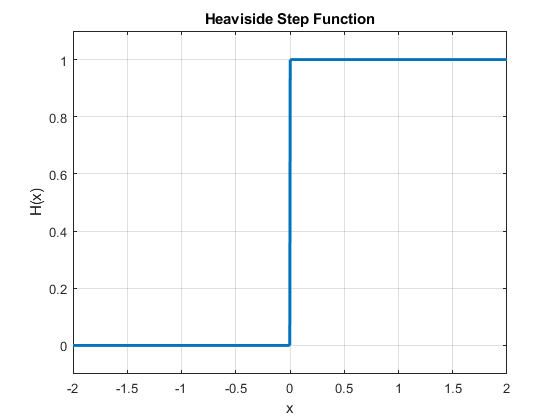
\includegraphics[width=4cm, keepaspectratio]{img/img-ch1/heaviside_graph.png}}\\
        Sigmoid & $\sigma (x) = \frac{1}{1+e^{-x}}$ & \adjustbox{valign=c}{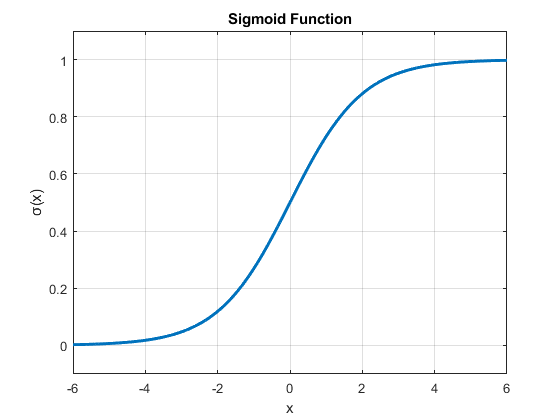
\includegraphics[width=4cm,keepaspectratio]{img/img-ch1/sigmoid.png}} \\
        ReLU & $\sigma(x)=\max\left\lbrace 0, x\right\rbrace $ & \adjustbox{valign=c}{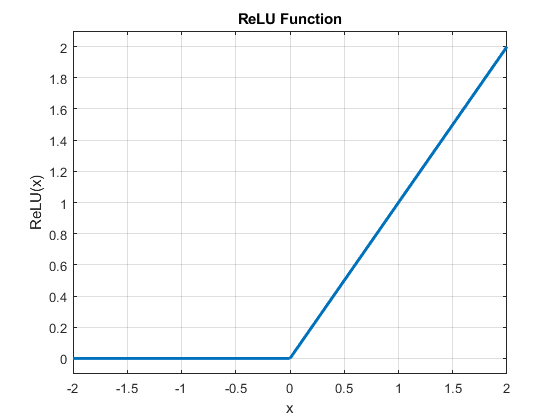
\includegraphics[width=4cm,keepaspectratio]{img/img-ch1/reLU.png}}\\
        Hyperbolic tangent & $\sigma(x)=\tanh (x)$ & \adjustbox{valign=c}{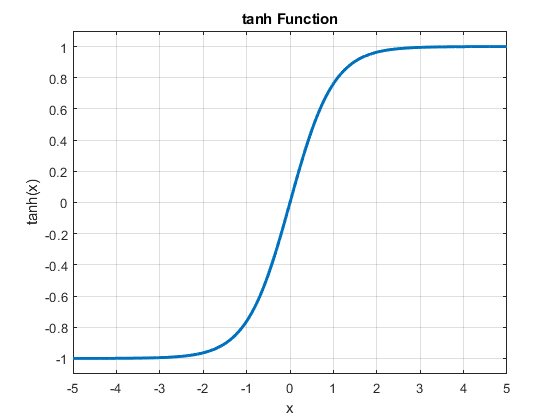
\includegraphics[width=4cm,keepaspectratio]{img/img-ch1/tanh.png}}\\
    \end{tabular}
    \caption{Activation functions}
    \label{tab:activation_functions}
\end{table}

The graphical representation of neural networks (such as \autoref{fig:neural_network}) really helps describing and visualizing its architecture because it intuitively presents information ``flowing'' from the inputs on the far left, along links and through hidden nodes, ultimately to output $f(x)$ on the far right. In order to avoid confusion with the notation, we will make an effort to detail it now that will reward us in the next sections.

Neural networks connect multiple neurons in layers, labeled by $l=0,...,L$ so that the units of each layer are connected to the units of the following layer. In the example of \autoref{fig:neural_network}, $L=3$: the input layer $l=0$, the output layer $l=L$ which determines the value of the function and the layers in between $1 \leq l<L$ are hidden layers. The first layer is formed by input units $x_1,...,x_N$, the following $L-1$ layers contain the hidden neurons $h_{1}^{(l)},...,h_{J_{l}}^{(l)}$ where $l=1,...,L$ and $J_{l}$ is the number of neurons of the $l$-th hidden layer. The last layer consists on the output unit(s). It is common to add a bias term in the weighted sum of the inputs of a neuron, resulting in an extra unit in each layer with fixed value $1$, so that the bias parameter $b$ is taken into account in the computations.

Every arrow represents a weight or connection strength from a neuron in a layer to a neuron in the next layer. The weights are represented by $W_l, \, l=1,...,L$, a real valued matrix of weights of the $l$-th layer. The weight into neuron $j$ in layer $l$ from node $i$ in the previous layer $l-1$ is $w_{l}^{(i \rightarrow j)}$. Each neuron is updated by an activation function depending on all neurons feeding into it, and the update protocol prescribes that each layer is updated after the previous one, thus working layer by layer. When working this way, vector and matrix notation are useful: the output of neurons $1,...,J_l$ in layer $l$ is the vector $X_l \in \left\lbrace 1 \right\rbrace \times \mathbb{R}^{J_l}$ and the matrix of weights $W_l$ of dimension $(J_{l-1}+1) \times J_l$ (taking into account the bias node).

The dimension of each layer $d = [J_{1}, J_{2},..., J_{L}]$ and the number of layers $L$ determines the architecture of the neural network, which means the neural network model family whose parameters will be optimized to choose the specific configuration of weights that best generalises the data.

\begin{figure}
    \centering
    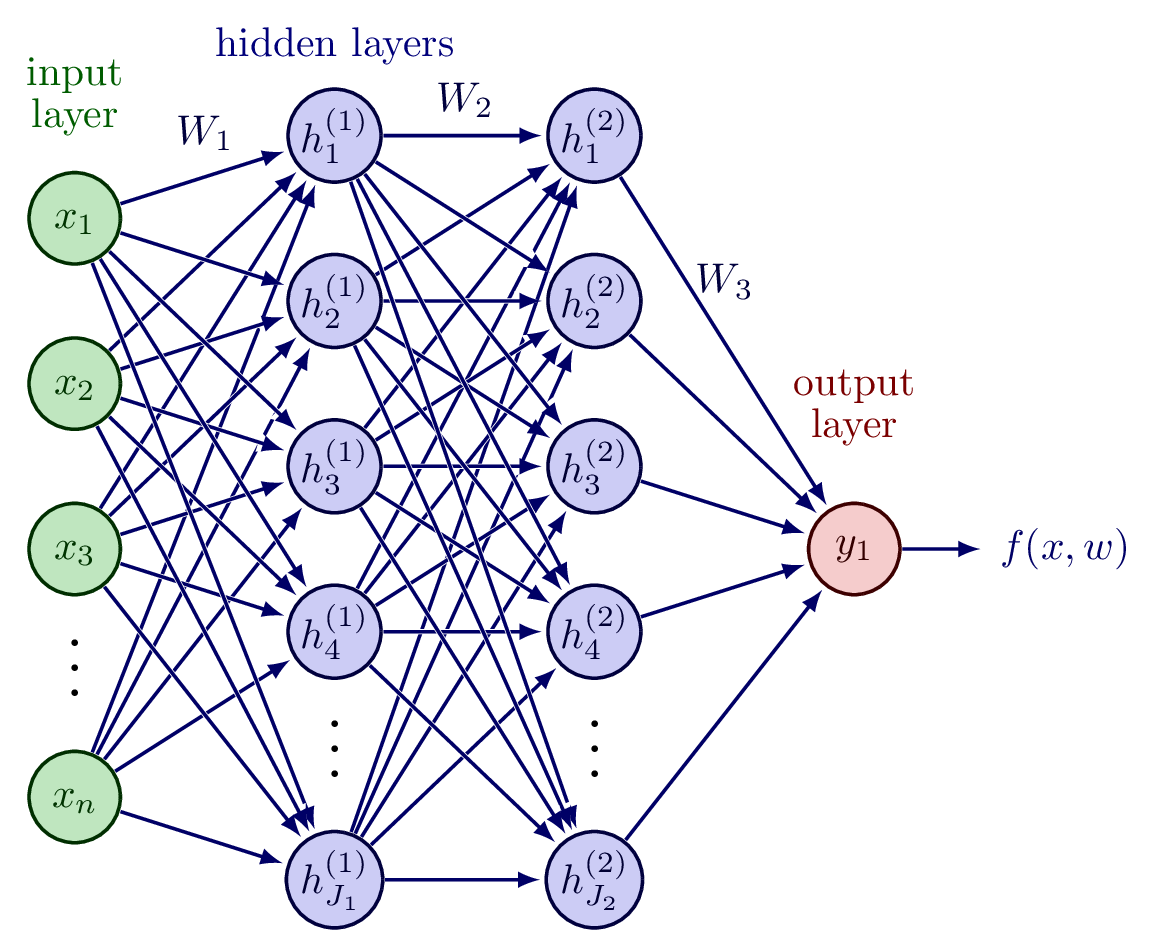
\includegraphics[width=0.8\linewidth]{img/img-ch1/NN.png}
    \caption{Illustration of a neural network. Adapted from \href{https://tikz.net/neural_networks/}{Izaak Neutelings}, \href{https://creativecommons.org/licenses/by-sa/4.0/}{CC BY-SA 4.0}}
    \label{fig:neural_network}
\end{figure}

\subsection{Forward propagation}
The function that expresses the output of a neural network is
\begin{equation}
    f_{W_1, W_2,..., W_L}(x) = \varphi_L(w_L \varphi_{L-1}(W_{L-1} \cdots \varphi_2(W_2 \varphi_1(W_1 x) ) \cdots ) )
\end{equation}
where $x \in\mathcal{X}$, $W_i, \, i=1,...,L$ is a real valued matrix of weights of the $i$-th layer and $\varphi_i$ is the activation function in vectorised form. This is computed by the \textbf{forward propagation algorithm}. Taking into account the bias as node 0, we can observe that the inputs and outputs of a layer are related by
\begin{equation}
    X_l = \begin{bmatrix}
        1 \\
        \sigma(W_l X_{l-1})
    \end{bmatrix} 
\end{equation}
where $\sigma(W_l X_{l-1})$ is a vector whose components are the result of applying the vectorised form of the activation function to the weighted sum (with weights $W_l$) of the outputs from the previous layer ($X_{l-1}$)

This computation starts by initializing the input layer $x_1 = x \in \mathcal{X}$. 

After forward propagation, the output vector $x_l$ at every layer $l=1,...,L$ has been computed. 

\subsection{Backpropagation Algorithm}
Gradient descent is the algorithm used for finding the minimum of a differentiable function. It iteratively updates the parameters $\theta$ of a cost function $C(\theta)$ towards the direction of steepest descent in order to minimize a cost function. In the case of neural networks, the cost function and the model function of the neural network depend on $W = \left\lbrace W_1, ,..., W_L\right\rbrace$. Considering the squared error loss and the dataset $\mathcal{D}=\left\lbrace (x_1,y_1),...,(x_M,y_M)\right\rbrace$, we will work with the following cost function:
\begin{equation}
    C(W)=\frac{1}{M} \sum_{i=1}^M (f(x_i,W)-y_i)^2
\end{equation}

The gradient descent algorithm is our preferred choice for performing the optimisation of the parameters since, when working with nonlinear activation functions, we are facing a difficult optimisation problem that generally is nonlinear and non-convex. The weights are updated in gradient descent at every step $t=1,2,...$ in the following way
\begin{equation}
    W(t+1)=W(t) + \eta \nabla C(W(t))
\end{equation}

To perform gradient descent we need the gradient and to compute the gradient of $C(W)$, we need its derivative with respect to each weight matrix
$$\frac{\partial C}{\partial W_l} = \frac{1}{M}\sum_{i=1}^M \frac{\partial e_n}{\partial W_l}$$
where $e_n=(f(x_n,W)-y_n)^2$

We could think of obtaining $\frac{\partial e}{\partial W_l}$ using the finite differences numerical method. Taking into account we need to compute this method for every weight and for every data point, it becomes computationally prohibitive. The alternative that enables us to compute these gradients is a dynamic programming algorithm known as backpropagation. It is based on several applications of the chain rule. Next, we will deduce the algorithm step by step and then, we will be able to join all the pieces together to write its pseudo-code.

We want to obtain the partial derivative $\frac{\partial e}{\partial W_l}$

First, observe that variations on the weights $W_l$ influence the output $X_L$ of the neural network. We can view schematically this dependency
$$W_l X_{l-1} \stackrel{\sigma}{\longrightarrow} X_l \longrightarrow W_{l+1}X_l \stackrel{\sigma}{\longrightarrow} X_{l+1} \longrightarrow \cdots \longrightarrow X_L = f(x, W) $$
From now on, we will call $W_l X_{l-1}=S_l$, that is, the input of the $l$-th layer. This vector $S_l = [s_{(l),j}]_{j=1}^{J_l}$ corresponds to the inputs of each $j$ node of the $l$-th layer.

Since variations in $W_l$ impact the output $f(x,W)$, in turn, it affects the loss error $e$. Let's view this effect of $W_l$ element-wise. A change in $w_l^{i\rightarrow j}$ only affects $s_{(l),j}$ the input of the $j$-th node of the $l$-th layer because $$s_{(l),j} = \sum_{i=0}^{J_{L-1}}w_l^{i\rightarrow j}x_{(l-1),i}$$
Thus, by the chain rule
\begin{equation}
    \frac{\partial e}{\partial w_l^{i\rightarrow j}} = \frac{\partial s_{(l),j}}{\partial w_l^{i\rightarrow j}} \frac{\partial e}{\partial s_{(l),j}} = x_{(l-1),i} \delta_{(l),j}
\end{equation}
where the last equality follows from the linear relation between $s_{(l),j}$ and $w_l^{i \rightarrow j}$. We have defined $$\delta_{(l),j} = \frac{\partial e}{\partial s_{(l),j}}$$
The vector $$\delta_l = [\delta_{(l),j)}]_{j=1}^{J_l} = \frac{\partial e}{\partial S_{l}}$$ denotes the sensitivity and it quantifies how the error $e$  changes with $S_l$. 

We can obtain $X_{l}$ for every $l=1,...,L$ using forward propagation. So to get the partial derivatives, we need to obtain the sensitivity vectors $\delta_l$ for every layer. It turns out that the sensitivity vectors can be retrieved by ``running backwards'' our neural network. We can explicitly get the sensitivity of the output layer $\delta_L$ because $e=(X_L-y)^2 = (\sigma(S_L)-y)^2$. Therefore,
\begin{align}
    \delta_L &=\frac{\partial e}{\partial S_L} \\
    &= \frac{\partial}{\partial S_L} (X_L -y)^2 \\
    &= 2(X_L-y)\frac{\partial X_L}{\partial S_L} \\
    &= 2(X_L-y)\sigma^\prime(S_L)
\end{align}
is the starting point of the backward recursion.

We will see how to obtain $\delta_{(l),j}$ element-wise. Since $e$ depends on $S_l$ only through $X_l$, by the chain rule
\begin{align}
    \delta_{(l),j} &= \frac{\partial e}{\partial s_{(l),j}} \\
    &= \frac{\partial e}{\partial x_{(l),j}}\frac{\partial x_{(l),j}}{\partial s_{(l),j}} \\
    &= \frac{\partial e}{\partial x_{(l),j}} \sigma^\prime (s_{(l),j})
\end{align}

Next, we will obtain the partial derivative $\frac{\partial e}{\partial X_l}$. A variation in $X_l$ only affects $S_{l+1}$ and thus, $e$. A particular component of $X_l$ can affect every component of $S_{l+1}$, therefore we need to apply the chain rule taking into account all these dependencies:
\begin{align}
    \frac{\partial e}{\partial x_{(l),j}} &= \sum_{k=1}^{J_{l+1}} \frac{\partial s_{(l+1),k}}{\partial x_{(l),j}} \frac{\partial e}{\partial s_{(l+1),k}} \\
    &= \sum_{k=1}^{J_{l+1}} w_{l+1}^{j \rightarrow k} \delta_{(l+1), k}
\end{align}

because
\begin{itemize}
    \item $s_{(l),j} = \sum_{i=0}^{J_{L-1}}w_l^{i\rightarrow j}x_{(l-1),i}$ , 
    then its derivative with respect to $x_{(l-1),j}$ is 
    $$\frac{\partial s_{(l),k}}{\partial x_{(l-1),j}} = w_{l}^{j \rightarrow k}$$

    \item and by definition we have that
    $$\delta_{(l+1),k} = \frac{\partial e}{\partial s_{(l+1),k}} $$
\end{itemize}

Joining it all together, we obtain the expression for the components of the sensitivity vector
\begin{equation}
    \delta_{(l),j} = \sigma^{\prime}(s_{(l),j}) \sum_{k=1}^{J_{l+1}} w_{l+1}^{j\rightarrow k} \delta_{(l+1),k}
\end{equation}
This resulting equation to compute the sensitivity at the $l$-th layer is expressed in terms of the sensitivity in the next layer $l+1$, producing a backward recursion. Therefore, if we know the sensitivities at layer $l+1$, we can get $\delta_l$. 

The consequent vector expression of the sensitivity is
\begin{equation}
    \delta_l = \sigma^{\prime}(S_l) \odot [(W_{l+1})^T\delta_{l+1}]_{1}^{J_l}
\end{equation}
where $\odot$ denotes the Hadamard product, the elementwise product of the two vectors: \\ $u,v \in \mathbb{R}^n$, then $u \odot v $ is a vector such that $ (u \odot v)_i =u_i v_i, \, i = 1,...,n$. 

In the vector equation of the sensitivity $\delta_l$ in terms of the sensitivity in the next layer $\delta_{l+1}$, $W_{l+1}$ is the transpose of the weight matrix of the $l+1$-th layer, $W_{l+1}$. When we apply this transpose weight matrix we can think intuitively as moving the sensitivity error backward through the network. Then, we can interpretate the Hadamard product of $\sigma^{\prime}(S_l)$ as moving the sensitivity error backwards through the activation function in layer $l$. 

\begin{tcolorbox}[title=Backpropagation algorithm]
    \textbf{Input:} a data point $(X,y)$
    \begin{enumerate}
        \item Run forward propagation on $X$ to compute and save $X_l$ and $S_l$ for $l=1,...,L$

        \item \textbf{Initialization} 
        
        $\delta_L \leftarrow 2(X_L - y)\sigma^{\prime}(S_L)$

        \item \textbf{Backpropagation recursion}

        for $l=L-1$ to $1$ do:
        
        \qquad $\delta_l \leftarrow \sigma^{\prime}(S_l) \odot [(W_{l+1})^T\delta_{l+1}]_{1}^{J_l}$
    \end{enumerate}
    
\end{tcolorbox}


Finally, as a recapitulation, we will remember our goal was to perform gradient descent to optimise the weights of the neural network, for which we needed the gradient of the cost function with respect to every weight parameter. Using the chain rule, the expression for the required partial derivatives is
\begin{equation}
    \frac{\partial e}{\partial w_l^{i\rightarrow j}} = x_{(l-1),i} \delta_{(l),j}
\end{equation}

We can compute it because we can obtain the term $X_l,\, l=1,...,L$ with the forward propagation recursion
\begin{equation}
    X_l = \begin{bmatrix}
        1 \\
        \sigma(W_l X_{l-1})
    \end{bmatrix} 
\end{equation}
with initial condition $X_0=X\in \mathcal{X}$, the input vector.

On the other hand, we can calculate the sensitivities $\delta_l, \, l=1,...,L$ with backpropagation using the recursion 
\begin{equation}
    \delta_l = \sigma^{\prime}(S_l) \odot [(W_{l+1})^T\delta_{l+1}]_{1}^{J_l}
\end{equation}
with initial condition $\delta_L = 2(X_L - y)\sigma^{\prime}(S_L)$.



\endinput
%--------------------------------------------------------------------
% FIN DEL CAPÍTULO. 
%--------------------------------------------------------------------

% !TeX root = ../tfg.tex
% !TeX encoding = utf8

\chapter{Introduction to Quantum Computing} \label{ch:2-IntroQC}



In 1981 at MIT, the first Physics of Computation Conference was held, organized by MIT and IBM, which brought together 50 scientists for three days. It was the founding forum to discuss the possibility of taking signals from the natural world to address the problems of designing increasingly powerful and efficient forms of computation. Attendees debated the limitations and possibilities brought about by the shrinking of computer components (Moore's Law). Ultimately, it was the time and place to discuss the intersection of the physical sciences and computer sciences, which helped to connect the paths of both disciplines. Today, this conference holds more weight than they could have imagined at the time. Perhaps due to the significance of its sponsoring institutions and the fame of some attendees, such as Freeman Dyson, John Wheeler, and Richard Feynman, we can say that it was the birthplace of physics of computation and especially the now flourishing field of quantum computing.

The opening speech of the Physics of Computation Conference was delivered by Richard Feynman and was titled ``Simulating physics with computers''. As the title suggests, it explores the idea of how physics can be simulated using computers, which is related to the possibilities of computers and also the possibilities of physics. Throughout the speech, he poses a series of questions.

First, he addresses the question: What type of physics will be simulated with computers? Classical physics is often described using differential equations, but the physical world is quantum, so the problem he raises is simulating quantum physics.

\begin{quote}
    ``And I'm not happy with 
all the analyses that go with just the classical theory, because nature isn't 
classical, dammit, and if you want to make a simulation of nature, you'd 
better make it quantum mechanical, and by golly it's a wonderful problem, 
because it doesn't look so easy."
\end{quote}

The idea that Richard Feynman explores is whether there is an exact simulation in which the computer will do exactly the same as nature.

So, how can quantum mechanics be simulated? To answer this question, Richard Feynman concludes that the only possibilities are: to use a probabilistic computer or to do it with a new type of computer, a quantum computer built with elements of quantum mechanics that obey the laws of quantum mechanics. He asserts that a quantum system can be simulated with quantum computational elements. He is not referring to a Turing machine but to a machine of a different type. Feynman believes that it is true that with an appropriate class of quantum machines, one could simulate any quantum system, including the physical world.

In his speech, Feynman only outlines ideas about what this quantum computer would be like. He also raises the question of which types of quantum systems are equivalent and the possibility of finding a class that could simulate all quantum systems. This leads to the question of whether a universal quantum computer could be found. He suggests using linear operators in a two-state quantum system as the basis for simulating any quantum system.

In the final part of the conference, he argues whether a quantum system can be probabilistically simulated with a classical universal probabilistic computer, meaning a computer that would obtain the same probabilities as the quantum system. He concludes that this is definitely not the case and that it is impossible to represent the results of quantum mechanics with a classical universal device.

Feynman proposes this union between computing and physics because he claims that the discovery of computing has proven very useful in many branches of human reasoning. For example, attempting to create a computer that understands our language made us realize how poor our understanding of language and grammar theory was. Similarly, we have gained some insights about psychology and philosophical issues by approaching them from a computational perspective. Feynman's intention was that introducing computational approach would provide us with new ideas if they were necessary.

\section{Review on Hilbert spaces}
Quantum theory can me understood as an extension of classical probability theory to make predictions about the stochastic outcomes of measurements on microscopic objects (such as electrons, protons, atoms, etc.) that form quantum systems.

The rigorous formulation of this requires some mathematical tools and notions that we will review next.

\begin{definicion}[Inner product]
    Let X be a vector space, that is, 
    \begin{equation*}
        \psi,\phi \in X \text{ and } a,b \in \mathbb{C} \text{ verify } a\psi+b\phi \in X
    \end{equation*}
    The scalar product or inner product in $X$ is an application 
    \begin{align*}
        \braket{\cdot,\cdot}:X\times X &\longrightarrow \mathbb{C} \\
        (\psi, \phi) &\longmapsto \braket{\psi,\phi}
    \end{align*}
    That verifies for all $\phi, \psi, \phi_1, \phi_2 \in X$ y $a,b\in \mathbb{C}$
        \begin{enumerate}
            \item It is hermitian: $\braket{\psi,\phi} = \overline{\braket{\psi,\phi}}$ 
            \item It is positive definite: $\braket{\psi,\psi}\geq 0$ y $\braket{\psi,\psi}=0 \Leftrightarrow \psi = 0$
            \item It is sesquilinear, that is
                \begin{itemize}
                    \item $\braket{\psi,a\phi_1+b\phi_2}=a\braket{\psi,\phi_1}+b\braket{\psi,\phi_2}$ (Linearity of the second entry)
                    \item $\braket{a\psi_1 + b\psi_2,\phi}=\overline{a}\braket{\psi_1,\phi}+\overline{b}\braket{\psi_2,\phi}$ (Antilinearity of the first entry)
                \end{itemize}
        \end{enumerate}
\end{definicion}

\begin{definicion}[Pre-Hilbert space]
    If $\braket{\cdot , \cdot}$ is a inner product in a vector space $\mathbb{H}$, we will say that $\mathbb{H}$ is a pre-Hilbert space.
\end{definicion}

This inner product induces a norm in $\mathbb{H}$, 
\begin{align}
    || \cdot ||:\mathbb{H} &\longrightarrow \mathbb{R}\\
    \psi &\longmapsto \sqrt{\braket{\psi,\psi}}
\end{align}

\begin{definicion}
    A normed space $M$ is complete if every Cauchy sequence in $M$ is convergent. That is, if $\left\lbrace x_n\right\rbrace_{n \in \mathbb{N}}$ is a sequence in $M$ such $\forall \epsilon >0\,\,\exists n_0 \in \mathbb{N}$ that $n,m \geq n_0$, $||x_n - x_m|| < \epsilon$, then $\left\lbrace x_n \right\rbrace$ converges in $M$. 
    This spaces receive the name of \textbf{Banach spaces}. 
\end{definicion}

\begin{definicion} [Hilbert space]
    A Hilbert space $\mathbb{H}$ is a pre-Hilbert space that is complete respect to the norm induced by the inner product.
\end{definicion}

Equivalently, a Hilbert space is a Banach space with the norm induced by the inner product. 

\begin{definicion}[Separable space]
    A metric space $M$ is separable if there exists a subset $N \subset M$ that is countable and dense.
\end{definicion}

Now we will quickly revise the basic concepts of linearly independence, span and basis.
\begin{definicion}
    Let $X$ be a pre-Hilbert space and $J$ an index set.
    
    A set of vectors $\left\lbrace v_i \, | \, i \in J\right \rbrace \subset X$ is \textbf{linearly independent} if the coefficients $\alpha_i \in \mathbb{C},\, i \in J$ such that
    $$\sum_{i \in J}\alpha_i v_i = 0$$
    only holds if $a_i=0$ for all $i\in J$.
    
    A set of vectors $\left\lbrace v_i \, | \, i \in J\right \rbrace \subset X$ \textbf{spans} X if for every $\omega \in X$, there are coefficients $\alpha_i \in \mathbb{C}$ , $ i\in J$ such that
    $$\omega =\sum_{I \in J} \alpha_i v_i$$ Therefore, we denote it as $$X = \mathrm{span}\left\lbrace v_i \, | \, i \in J\right \rbrace$$

    A linearly independent set $\left\lbrace v_i \, | \, i \in J\right \rbrace$ that spans $X$ is called a \textbf{basis} of $X$. 

    An \textbf{orthonormal basis} $\left\lbrace e_i \,\, | \, i \in J\right \rbrace $ is a basis whose vectors are unitary ($||e_i||=1\, \forall i \in J$) and verify
    $$\braket{e_i|e_j}=\delta_{i,j}=
    \left\{ \begin{array}{lcc} 
    0 & \mathrm{if} & i \neq j \\
    1 & \mathrm{if} & i = j 
    \end{array} \right.$$
\end{definicion}

\begin{teorema}
    Every separable Hilbert space has an orthonormal basis.
\end{teorema}
\begin{proof}
    Let $\mathbb{H}$ be a Hilbert space and $\left\lbrace u_n \right\rbrace$ be a countable dense subset of $\mathbb{H}$. We consider the nondecreasing sequence of linear spaces $\left\lbrace E_i \right\rbrace = \textbf{span}\left\lbrace u_1, u_2, ..., u_i\right\rbrace$ such that $ \bigcup_{i=1}^{\infty} E_i$ is dense in $\mathbb{H}$. 

    Let's pick any unit vector $u_1$ in $E_1$. If $E_2 \neq E_1$, there is some vector $u_2 \in E_2$ such that $\left\lbrace u_1, u_2 \right\rbrace$ is an orthonormal basis of $E_2$. By repeating this iterative construction, we obtain an orthonormal basis of $\mathbb{H}$. \cite{brezis2011functional}
\end{proof}

Now we will get introduced to the notion of linear functional.

\begin{definicion}[Linear operator]
    Let $X$ and $Y$ be to vector spaces. A linear operator from $X$ to $Y$ is an application $T: X \longrightarrow Y$ that verifies
    $$T(\lambda_1 x_1 + \lambda_2 x_2) = \lambda_1 T(x_1) + \lambda_2 T(x_2) \quad \forall \lambda_1, \lambda_2 \in \mathbb{K},\,x_1, x_2 \in X$$

    If $Y = \mathbb{K}$ the linear operator $T$ receives the name of \textbf{linear functional}.
\end{definicion}

\begin{proposicion}[Continuous operator]
    Let $X$ and $Y$ be normed vector spaces and $T: X \longrightarrow Y$  a linear operator. Then $T$ is continuous if and only if $\exists M \in \mathbb{R}_0^{+}$  such that $$||T(x)|| \leq M ||x|| \quad \forall x \in X$$
\end{proposicion}

\begin{definicion} [Operator space]
    Given $X$ and $Y$ normed vector spaces over $\mathbb{K}$, we denote $\mathcal{L}(X,Y)$ the set of all linear operators from $X$ to $Y$. Provided with the operations:
    \begin{itemize}
        \item $\forall T,S \in \mathcal{L}(X,Y), \, (T+S)(x) = T(x) + S(x) \quad \forall x \in X$
        \item $\forall \lambda \in \mathbb{K},\,\forall T \in \mathcal{L}(X,Y), \, (\lambda T)(x) = \lambda T(x) \quad \forall x \in X$
    \end{itemize}
    The set $\mathcal{L}(X,Y)$ has structure of vector space. 
\end{definicion}

\begin{definicion}[Dual space]
    Let $X$ be a normed vector space over $\mathbb{K}$. The operator space from $X$ to $\mathbb{K}$, $\mathcal{L}(X,\mathbb{K})$ of all linear and continuous functionals in $X$ is called dual space and it is denoted as $X^{*}$. It is provided with the norm
    
    $$||f||_{X^{*}} = \min \left \lbrace M \in \mathbb{R}_0^{+} :\, |f(x)| \leq M||x||_{X} \quad \forall x \in X \right\rbrace$$
\end{definicion}


In a Hilbert space, we can define linear functionals $T_{\psi}$ for every $\psi \in \mathbb{H}$ with the help of the scalar product:
\begin{align}
    T_{\psi}: &\mathbb{H} \longrightarrow \mathbb{C} \\
    &\varphi \longmapsto \braket{\psi, \varphi}
\end{align}

By virtue of the Theorem of Riesz,  \autoref{th:Riesz theorem}, for each functional $T \in \mathbb{H}^{*}$, there exists a unique $\psi \in X$ such that $T(x)=\braket{x,\psi}\quad \forall x \in X$. 

This means that there is a bijection between $\mathbb{H}$ and its dual space $\mathbb{H}^{*}$: every linear and continuous functional from $\mathbb{H}$ to $\mathbb{C}$ is uniquely represented as a scalar product with a suitable vector in $\mathbb{H}$.

Therefore, $\mathbb{H}$ and $\mathbb{H}^{*}$ are isomorphic, in particular, if $\mathbb{H}$ is a separable Hilbert space, the dual space $\mathbb{H}^{*}$ is a vector space with the same dimension as $\mathbb{H}$.

This fact suggests the \textbf{Bra-ket notation} introduced by Paul Dirac, extensively used in Quantum Mechanics.
\begin{itemize}
    \item Ket-vectors are elements of $\mathbb{H}$. A vector $\varphi \in \mathbb{H}$ in the Hilbert space is denoted in Dirac's notation as the ket $\ket{\varphi} \in \mathbb{H}$.

    \item Bra-vectors are elements of the dual space $\mathbb{H}^{*}$. A functional $T_{\phi} \in \mathbb{H}^{*}$ is denoted in Dirac's notation as the bra $\bra{\phi} \in \mathbb{H}^{*}$.

    \item The action of a functional $\bra{\phi} \in \mathbb{H}^{*}$ on a vector $\ket{\varphi} \in \mathbb{H}$ is denoted as the braket $\braket{\phi | \varphi} = \braket{\phi, \varphi} \in \mathbb{C}$. Note the scalar product.
\end{itemize}

In other words, every ket $\ket{\varphi}$ has a corresponding $\bra{\varphi}$ that is unique. The scalar product of two vectors (kets) $\ket{\phi}$ and $\ket{\varphi}$ is given by the braket $\braket{\phi | \varphi}= \braket{\phi , \varphi}^{*}$

A basis of the Hilbert space $\mathbb{H}$ can be denoted according to Dirac's notation as $\left\lbrace \ket{\phi_i} \, | \, i \in J \right\rbrace$ and we can express any ket $\ket{\varphi} \in \mathbb{H}$ as 
$$\ket{\varphi} = \sum_{i \in J}\ket{\phi_i} \alpha_i$$
where $\alpha_i$ are the components of $\ket{\varphi }$ in the basis $\left\lbrace \ket{\phi_i} \, | \, i \in J \right\rbrace$.

Now, let $\left\lbrace \ket{e_i} \, | \, i \in J \right\rbrace$ be an orthonormal basis of $\mathbb{H}$. The coefficients of any vector can be obtained from the inner product, since $\ket{\varphi} = \sum_{i \in J}\ket{e_i} \alpha_i $, then
$$\braket{e_k|\varphi}= \sum_{i \in J}\braket{e_k|e_i} \alpha_i = \sum_{i \in J} \delta_{ki}\alpha_i = \alpha_k$$

As a result,
$$\ket{\varphi} = \sum_{i \in J}\ket{e_i} \braket{e_i|\varphi}$$

Regarding the inner product of two vectors, we can use its representation in an orthonormal basis as
\begin{align}
    \ket{\varphi} &= \sum_{i \in J}\ket{e_i} \varphi_i = \sum_{i \in J}\ket{e_i} \braket{e_i|\varphi} \\
    \ket{\phi} &= \sum_{i \in J}\ket{e_i} \phi_i = \sum_{i \in J}\ket{e_i} \braket{e_i|\phi}
\end{align}
$$\braket{\phi | \varphi} = \sum_{i \in J}\braket{\varphi | e_i} \braket{e_i|\phi} = \sum_{i \in J}\braket{e_i | \varphi}^{*} \braket{e_i|\phi} = \sum_{i \in J}\varphi_i^{*} \phi_i = \braket{\varphi, \phi}^{*} $$

Indeed, the isomorphism between $\mathbb{H}$ and $\mathbb{H}^{*}$ is given by the adjoint relation:
\begin{align}
    \mathbb{H} &\longrightarrow \mathbb{H}^{*} \\
    \ket{\varphi} &\longmapsto \bra{\varphi} = \ket{\varphi}^\dag =\sum_{i \in J} \varphi_i^{*} \bra{e_i}
\end{align}
Thus, there is an adjoint basis in $\mathbb{H}^{*}$
$$\left\lbrace \ket{e_i}\right\rbrace  \longmapsto \left\lbrace \bra{e_i}\right\rbrace$$

\begin{definicion}[Adjoint operator]
    Let $X$ and $Y$ be normed spaces. Consider the linear operator $T$ from $X$ to $Y$. The adjoint operator of $T$, noted as $T^\dag$ is the operator $T^\dag : Y^* \longrightarrow X^* $ defined as $\forall g \in Y^*,\, T^\dag (g)$ is the functional given by $(T^\dag g)(x) = g(T(x)) \quad \forall x \in X$. 
    When $X$ and $Y$ are finite spaces of dimension $n$, then $T \in \mathcal{M}_{n \times n}$. Thus, its adjoint $T^\dag$ is given by $(T^\dag)_{ij}= T^*_{ji}$. 
\end{definicion}

When $T$ is a linear operator in a Hilbert space $\mathbb{H}$, we can apply the Riesz theorem, \autoref{th:Riesz theorem}, on both sides of the definition $(T^\dag g)(x) = g(T(x))$ to obtain that the adjoint operator realices the following equivalent identity: $\braket{T^\dag (u) , v} = \braket{u, T(v)}, \, \forall v \in \mathbb{H}$.


\begin{definicion}[Self-adjoint operator]
    A linear operator $T$ in a Hilbert space $\mathbb{H}$ is a self adjoint operator, also known as Hermitian operator, if its adjoint is itself: $T^\dag =T$. This is equivalent to say $\braket{T(x), y} = \braket{x, T(y)} \quad \forall x, y \in \mathbb{H}$.
\end{definicion}

\begin{definicion}[Unitary operator]
    An operator $T$ is unitary if $T^\dag T = T T^\dag = \mathbb{1}$
\end{definicion}

\begin{definicion} [Outer product]
    Let $X$ and $Y$ be vector spaces. The outer product of $v \in X$ and $w \in Y$, using Dirac's notation is $$\ket{w} \bra{v}$$ is the only linear operator such that 
    $$(\ket{w} \bra{v}) \ket{x} = \braket{v,x} \ket{w} \quad \forall \ket{x} \in X$$.
\end{definicion}

Lastly, we will remember the concepts of eigenvalues and eigenvectors.

\begin{definicion}[Eigenvalue and eigenvector]
    Given $X$ a vector space over $\mathbb{K}$, $T \in \mathcal{L}(X)$ and $v \in X$. If there exist a $\lambda \in \mathbb{K}$ such that
    \begin{equation}
        T v = \lambda v
    \end{equation}

    Then, $\lambda$ is an eigenvalue of $T$ and $v$ is a eigenvector of $T$. 
\end{definicion}

Next, we will present two definitions that allow us to quantify the characteristics of a system defined within a Hilbert space.

\begin{definicion}[Observable]
    In physics, an observable, such as position or momentum, are physical quantities governed by a real-valued function in the case of classical mechanics. In the case of quantum mechanics, an observable is given by an operator that can be measured. 
\end{definicion}

\begin{definicion}[Expected value]
    Given an operator $T$, the expected value $\braket{T}$ is defined as the probabilistic value expected to be obtained when a measurement of the observable associated with $T$ is performed. If the system is in a state $\psi$, the expected value of $T$ is given by $\braket{T}_{\psi}=\braket{\psi | T | \psi}$.     
\end{definicion}

Finally, we will point out a particular type of observable:

\begin{definicion}[Hamiltonian]
    In quantum mechanics, the operator corresponding to the total energy (kinetic and potential) of the system is called the Hamiltonian.
\end{definicion}


\section{Postulates of Quantum Mechanics} \label{sec: postulates of QM}
Now, we will formulate the framework of quantum mechanics for finite-dimensional systems with the guidance of a number of postulates which specify the mathematical objects used to describe certain physical entities. We will follow \cite{nielsen_chuang_2010}.

\subsection{State space} \label{sec: state space}
\begin{tcolorbox}[title=Postulate $1$]

    Associated to any isolated physical system is a complex vector space with inner product (that is, a Hilbert space) known as the \textbf{state space} of the system. The system is completely described by its \textbf{state vector}, which is a unit vector in the system's state space.
\end{tcolorbox}

A quantum system with a state vector $\ket{\psi}$ is called a pure state. However, usually systems cannot be described by an unique pure state, instead they are in a statistical ensemble of different pure states, each of them with its own probability. In this case, the state of a system is given by a operator called \textbf{density operator} or \textbf{density matrix}, defined by
\begin{equation}
    \rho = \sum_{i=1}^{n} p_i \ket{\psi_i}\bra{\psi_i}
\end{equation}
where all $p_i \geq 0 $ and $\sum_i p_i = 1$.

Additionally, a density matrix has the following properties:
\begin{enumerate}
    \item $\rho$ is self-adjoint $$\rho^{\dag}=\rho$$
    \item $\rho$ has trace $1$ $$\mathrm{Tr}(\rho) = 1$$
    \item $\rho$ is positive $$\rho \geq 0$$
    
\end{enumerate}


This postulate does not provide the state space for a given system. Although, for the purpose of computation, the state spaces to consider should be discrete and finite-dimensional Hilbert spaces. These are isomorphic to the $\mathbb{C}^K$, and a quantum state therefore has a representation as a complex-valued vector.

The simplest quantum mechanical system is the one qubit system.

\begin{definicion}[Qubit]
    A state vector of the state space $\mathbb{C}^2$ is called a qubit.
\end{definicion}

Now we pick up again Dirac's notation and we assume $\ket{0}$ and $\ket{1}$ form an orthonormal basis in a 2-dimensional Hilbert space. Thus, any state vector in the state space can be written as a linear combination of the basis vectors:
$$\ket{\varphi} = \alpha \ket{0} + \beta \ket{1}$$

where $\alpha, \beta \in \mathbb{C} $ are called amplitudes. A state vector is by definition unitary. This condition translates into $\braket{\varphi | \varphi} = 1$, which is equivalent to $|a|^2 + |b|^2 = 1$. This is known as normalization condition. 

A qubit is the minimal information unit in quantum computing. It is the analogous to the classical bit in classical computation. Intuitively, the states $\ket{0}$ and $\ket{1}$ are equivalent to the values 0 and 1 which a bit may take. The difference relies on the fact that $\ket{0}$ and $\ket{1}$ are not the only states of a qubit, one can prepare a qubit in any arbitrary superposition of these two states: $\alpha \ket{0} + \beta \ket{1}$. 

As we know, classical computation is built based on bits. Similarly, quantum computing is constructed upon the qubit. 

We conclude with some usual terminology. The orthonormal basis of the state space receives the name of computational basis. In the case of the state space of a 1-qubit system, the constituents of the computational basis are the column vectors
\begin{equation}
    \ket{0} =
    \begin{bmatrix}
    1\\
    0\\
    \end{bmatrix}
    \quad \quad
    \ket{1} =
    \begin{bmatrix}
    0\\
    1\\
    \end{bmatrix}  
\end{equation}

and hence,
\begin{equation}
    \ket{\varphi}= \alpha \ket{0} + \beta \ket{1} = \alpha \begin{bmatrix}
    1\\
    0\\
    \end{bmatrix} + \beta \begin{bmatrix}
    0\\
    1\\
    \end{bmatrix} = \begin{bmatrix}
    \alpha\\
    \beta\\
    \end{bmatrix} 
\end{equation}

Additionally, taking into account a general orthonormal basis $\ket{e_i}$ of $\mathbb{H}$, with $\braket{e_i| e_j} = \delta_{ij}$, we realise that any $\ket{\varphi} \in \mathbb{H}$
$$\ket{\varphi} = \sum_i \braket{e_i|\varphi} \ket{e_i}$$

This previous equation also implies the \textbf{completeness relation}: $$\sum_i \ket{e_i}\bra{e_i} = \mathbb{1}$$ which holds for any orthonormal basis $\ket{e_i}$ of a finite $\mathbb{H}$.

We can generalise this to the case of $n$-qubits, thus we say that any linear combination $\sum_{i} \alpha_i \ket{\phi_i}$ is a superposition of the states $\ket{\phi_i}$ with amplitude $\alpha_i$ for the state $\ket{\phi_i}$.

In particular, we will see that the state space will be $\mathbb{C}^{2^n}$ for an $n$-qubit quantum computation system.

In conclusion, this first postulate sets the framework in which quantum mechanics takes place: Hilbert spaces. In particular, for quantum computation where we work with a finite number of qubits, we will consider finite Hilbert spaces. Linear algebra and functional analysis provide us the tools we need to operate in them. It is worth pointing out that the definition of a qubit is derived from quantum physics and mathematics, describing the qubit as a mathematical object independent of its physical implementation. This enables the construction of quantum computing regardless of its physical implementation.

\subsection{Observables} \label{sec: observables}
\begin{tcolorbox}[title=Postulate $2$]

    An observable, that is, a physically measurable quantity of a quantum system is represented by a Hermitian or self-adjoint operator on a Hilbert space $\mathbb{H}$.
\end{tcolorbox}

Let $\mathcal{M}$ be a self-adjoint operator in $\mathbb{H}$ that acts on ket $\ket{\varphi}$ characterising the system. By virtue of the spectral theorem, \autoref{th:spectral theorem}, such self-adjoint operators have a diagonal matrix representation in terms of the orthonormal basis of eigenvectors
 $\left\lbrace \ket{\mu_j} \right\rbrace$, with the eigenvalues in the diagonal.
We can formulate this like
\begin{equation}
    \mathcal{M}=\sum_{k} \lambda_k \ket{\lambda_k} \bra{\lambda_k}
\end{equation}
where $\lambda_k$ are the eigenvalues and $\ket{\lambda_k}$ their corresponding eigenvectors. 

The only possible values that the observable can take are its eigenvalues, which are real because the observable is a self-adjoint operator. Therefore, the values of physical observables are always real numbers.

\subsection{Time Evolution}\label{sec: time evolution}

\begin{tcolorbox}[title=Postulate $3$]

    The evolution of a closed quantum system is described by a unitary transformation. That is, the state $\ket{\varphi}$ of the system at time $t_1$ is related to the state $\ket{\varphi^\prime}$ of the system at time $t_2$ by a unitary operator $U$ which depends only on the times $t_1$ and $t_2$. 
    \begin{equation}
        \ket{\varphi^\prime} = U(t_1,t_2) \ket{\varphi}
    \end{equation}
\end{tcolorbox}

This postulate encloses how a quantum state $\ket{\varphi}$ evolves through time but it does not tell you which unitary operators describe this evolution. In the context of quantum computing, any unitary operator can be realized in realistic systems and we will define them. While we may not know the specific unitary transformation for an arbitrary system, we are able to create systems that follow specific desired transformations. These principles form the foundation of quantum gates and quantum circuits

Now we will have a look at an example of an unitary operator on a single qubit which is important in quantum computation. We will detail at the end of this chapter a collection with the most important quantum gates.

\begin{ejemplo}[NOT gate]
    Let's consider the operator given by the matrix 
    \begin{equation}
        X = \begin{bmatrix}
        0&1\\
        1&0\\
        \end{bmatrix} 
    \end{equation}
    known as the Pauli X matrix $\sigma_x$ or NOT gate. It is evidently a unitary operator, since $X^\dag X = \mathbb{1}$. 

    We can observe that 
    \begin{equation}
        X \ket{0}= \begin{bmatrix}
        0&1\\
        1&0\\
        \end{bmatrix} 
        \begin{bmatrix}
        1\\
        0\\
        \end{bmatrix} =
        \begin{bmatrix}
        0\\
        1\\
        \end{bmatrix} = \ket{1}
    \end{equation}
    which is precisely what Postulate 3 states,  the evolution
    of our state vector following the unitary operator $X$: $X \ket{0} = \ket{1}$. 
\end{ejemplo}

It is worth pointing out two aspects of this postulate.
\begin{itemize}
    \item It requires that the physical system system is closed, that is, it is not interacting in any way with the exterior. This is quite a strict assumption, since in reality, all systems interact at least somewhat with others and the only real closed system is the universe as a whole. However, some systems can be described to a good approximation as being closed.

    \item It refers to the description of evolution of a closed quantum system at two different times $t_1$ and $t_2$. It is natural to consider the evolution of a quantum system in continuous time. For this, we will consider the Schrödinger equation, which provides a continuous time description of a closed system. We can redefine the Postulate 3 in these terms.
\end{itemize}

\begin{tcolorbox}[title=Postulate $3^\prime$]

    The time evolution of the state of a closed quantum system is described by the Schrödinger equation,
    \begin{equation}
        i \hbar \frac{d \ket{\phi}}{dt} = H \ket{\phi}
    \end{equation}
    where $\hbar$ is a physical constant known as Plank's constant and $H$ is a fixed Hermitian operator known as the Hamiltonian of the closed system.
\end{tcolorbox}

The Hamiltonian of the system is fixed and it represents the energy of the system. The value $\hbar$ is physical constant that we can absorb into the Hamiltonian to simplify the equation. At the end of the day, a Hamiltonian is an observable and we can apply the results from Postulate 2. As we will see later, circuits in quantum computers are built up from elementary gates that act as unitary operators on the states. In order to implement such gates, one then tries to create Hamilton operators that generate a time evolution implementing the desired gate.


Since the Hamiltonian is a self-adjoint operator, by the Spectral decomposition theorem, \autoref{th:spectral theorem}
$$H = \sum_{j} \lambda_j \ket{\lambda_j} \bra{\lambda_j}$$
with eigenvalues $\lambda_j$ and corresponding eigenvectors $\ket{\lambda_j}$. Conventionally, $\ket{\lambda_j}$ are referred to as \textit{energy eigenstates} and the eigenvalues $\lambda_j$ as the energy of the state $\ket{\lambda_j}$. 

Now we will consider the example for a single qubit that has Hamiltonian $$H=\hbar \omega X, \quad \omega >0,\, 
        X = \begin{bmatrix}
        0&1\\
        1&0\\
        \end{bmatrix} $$
to check that there is a one to one correspondence between the continuous time-varying postulate $3^\prime$ using the Hamiltonian and the more stationary discrete-time version using the unitary operator (Postulate 3). 

The energy eigenstates of this Hamiltonian are the ones of $X$: \\$(\ket{0} + \ket{1})/\sqrt{2}$ and $(\ket{0} - \ket{1})/\sqrt{2}$ with corresponding energies (eigenvalues): $\hbar \omega$ and $-\hbar \omega$. 

The solution to Schrödinger's equation is
$$\ket{\phi(t_2)} = \exp{\left[ \frac{-i H(t_2-t_1)}{\hbar}\right] } \ket{\phi(t_1)}$$

Now, we define the operator 
$$U(t_1, t_1) = \exp{\left[ \frac{-i H(t_2-t_1)}{\hbar}\right] } \ket{\phi(t_1)}$$
which is an unitary operator. In fact, any unitary operator $U$ can be expressed as $U=\exp (iK)$ for some Hermitian operator K. 

Therefore, we obtain that the state $\ket{\phi(t_2)}$ is related with the state $\ket{\phi(t_1)}$ through the unitary operator $U(t_1, t_2)$:
$$\ket{\phi(t_2)} = U(t_1,t_2) \ket{\phi(t_1)}$$

Like this, we have obtained the equivalence of postulates $3$ and $3^\prime$.

In quantum computing, the circuit model usually consists of ``applying'' a unitary operator to a quantum system. A priori we may think that this act contradicts what we have just stated about the evolution of a closed quantum system because we are interacting with it and thus, the system is not closed. It turns out to be possible to write down a time-varying Hamiltonian for a quantum system that is not closed but overall the system evolves according to Schrödinger's equation with a time-varying Hamiltonian to some good approximation. The main exception to this are measurements, which we will dive into next.

\subsection{Measurements}\label{sec: measurements}
A closed quantum system evolves according to unitary evolutions by virtue of Postulate 3. But the moment there is an observation of the system, this interaction makes the system no longer closed and thus, not necessarily subject to unitary evolution. To explain what happens in this context we will introduce the following postulate, which describes the effects of measurement operations on quantum systems.

\begin{tcolorbox}[title=Postulate $4$]

    Quantum measurements are described by a collection $\left\lbrace M_m \right\rbrace$ of \textit{measurement operators}. These are operators acting on the state space of the system being measured. The index $m$ refers to the measurement outcomes that may occur in the experiment. If the state of the quantum system is $\ket{\phi}$ immediately before the measurement then the probability that result $m $ occurs is given by 
    $$p(m) = \braket{\phi | M_m^{\dag}M_m | \phi }$$
    and the state of the system after the measurement is 
    $$\frac{M_m \ket{\phi}}{\sqrt{\braket{\phi | M_m^{\dag}M_m | \phi }}}$$

    The measurement operators satisfy the \textbf{completeness equation}:
    $$\sum_m M_m^{\dag}M_m = \mathbb{1}$$
    
\end{tcolorbox}

The completeness equation expresses the fact that probabilities of the possible different outcomes sum one. 
    $$\sum_m p(m) = \sum_m \braket{\phi | M_m^{\dag}M_m | \phi } = \braket{\phi |\sum_m M_m^{\dag}M_m | \phi } = \braket{\phi|\phi} = 1$$
Reciprocally, the fact of every state verifying this equation implies the completeness equation.

In the context of quantum computing, an important measurement is the measurement in the computational basis. Now we will review it for the case of a single qubit. 

When measuring a qubit there are two possible outcomes: $\ket{0}$ and $\ket{1}$ defined by two measurement operators $M_0 = \ket{0}\bra{0}$ and $M_1=\ket{1} \bra{1}$ respectively. We can observe that:
\begin{itemize}
    \item These measurement operators are Hermitian: $$M_i^{\dag} = (\ket{i} \bra{i})^{\dag} = (\bra{i})^{\dag} (\ket{i)}^{\dag} = \ket{i} \bra{i} = M_i$$
    \item They verify $M_i^2 = \ket{i} \braket{i|i} \bra{i} = \ket{i} \bra{i} = M_i$
    \item The computational basis is orthonormal and thus, fulfills the completeness relation: 
    $$\sum_i \ket{i} \bra{i} = 1$$
    Then, the completeness equation also holds:
    $$\sum_i M_i^{\dag}M_i = \sum_i M_i^2 = \sum_i M_i = \sum_i \ket{i} \bra{i} = 1$$
\end{itemize}

Now, let's measure. Suppose we have the state $\ket{\phi} = \alpha \ket{0} + \beta \ket{1}$. The probability of obtaining measurement outcome $0$ is 
$$p(0)=\braket{\phi | M_0^{\dag}M_0 | \phi } = \braket{\phi | M_0 | \phi} = |\alpha|^2$$
Analogously, the probability of obtaining the measurement outcome $1$ is $p(1)=|\beta|^2$.

The completeness equation $|\alpha|^2 + |\beta|^2 = 1$ is fulfilled thanks to the state vector normalization condition. 

After measurement, depending on the measurement outcome $0$ or $1$, the state would change respectively to:
\begin{align}
    \frac{M_0 \ket{\phi}}{|\alpha|} &= \frac{\alpha}{|\alpha|}\ket{0} \\
    \frac{M_1 \ket{\phi}}{|\beta|} &= \frac{\beta}{|\beta|}\ket{1} 
\end{align}

Multipliers like $\frac{\alpha}{|\alpha|}$ which have modulus one, can be ignored so the two post-measurement states are effectively $\ket{0}$ and $\ket{1}$. Thus, in this example, if we measured a $0$, the post-measurement vector will be $\ket{0}$ and viceversa. Any measurements performed after the first one will yield exactly the same result. This behaviour is called \textit{qubit collapsing}: the measurement changes state of a qubit, collapsing it from its superposition of $\ket{0}$ and $\ket{1}$ to the specific state consistent with the measurement result.

There is a special class of measurements worth pointing out known as \textbf{projective measurements}. Many applications of quantum computation work primarily with projective measurements. 
\begin{definicion}[Projective measurement]
    A projective measurement is described by an observable, $\mathcal{M}$, a Hermitian operator on the state space of the system being observed. The observable has a spectral decomposition
    $$\mathcal{M}= \sum_m m P_m$$
    where $P_m$ is the projector onto the eigenspace of $\mathcal{M}$ with the eigenvalue $m$. The possible outcomes of the measurement correspond to the eigenvalues, $m$, of the observable. Upon measuring the state $\ket{\phi}$, the probability of getting result $m$ is given by
    $$p(m) = \braket{\phi|P_m|\phi}$$

    Given that outcome $m$ occured, the state of the quantum system immediately after the measurement is 
    $$\frac{P_m \ket{\phi}}{\sqrt{p(m)}}$$

    \begin{equation}
        \phi \equiv \text{State before measurement} \stackrel{\text{measurement}}{\longrightarrow} \frac{P_m \ket{\phi}}{\sqrt{p(m)}} \equiv \text{state after measurement}
    \end{equation}
\end{definicion}

Projective measurements can be understood as a special case of Postulate 4. In addition, we can quickly realise that projective measurements are orthogonal ($\mathcal{M}_m \mathcal{M}_{m^\prime} = \delta_{m m^\prime} \mathcal{M}_m$) and satisfy the completeness equation ($\sum_m \mathcal{M}_m^{\dag} \mathcal{M}_m = \mathbb{1}$). Consequently, Postulate 4 reduces to a projective measurement.

These kind of measurements have nice properties and simplify the calculation of average values of the measurements. By definition, the average value of a measurement is the expected value, which for a discrete variable is a weighted average of the values of the variable, with weights given by the probabilities of each value:
\begin{align}
    \mathbf{E}(\mathcal{M}) &= \sum_m m p(m) \\
    &= \sum_m m \braket{\phi | P_m | \phi} \\
    &= \braket{\phi | \left( \sum_m m P_m \right) | \phi}\\
    &= \braket{\phi | \mathcal{M} | \phi}
\end{align}

A last remark regarding projective measurements is that usually, rather than giving an observable $\mathcal{M}$ to describe a projective measurement, we can provide a complete set of orthogonal projectors $P_m$ satisfying the relations $\sum_m P_m = \mathbb{1}$ and $P_m P_{m^\prime} = \delta_{m m^\prime}P_m$. The corresponding observable implicitely defined by its projectors is $\mathcal{M}=\sum_m m P_m$. The notion of ``measuring in a basis $\left \lbrace \ket{m} \right \rbrace$'' is also commonly used. Considering $\left \lbrace \ket{m} \right \rbrace$ that form an orthonormal basis, this measurement simply performs the projective measurement with projectors $P_m=\ket{m}\bra{m}$ and thus, the observable is $\mathcal{M}=\sum_m m \ket{m} \bra{m}$.

To conclude this section, the most important aspect to grasp from this postulate is the big difference between classic and quantum measurements. The measured state changes after the measurement. This means that the mere act of observing the system interferes with it. This intriguing aspect is one of the fundamentals of quantum mechanics.


\subsection{Composite systems}\label{sec: composite systems}

So far, we have worked with quantum systems of one qubit. But the real power of quantum computing is exploited when we are operating with composite quantum systems made up of two (or more) distinct qubits. We introduce the last postulate, which allows us to comprehend the state space associated with a physical system comprised of smaller subsystems. This will enable us to study the particular case of quantum computing systems made up of multiple qubits.

First we need to introduce the concept of \textbf{tensor product}. We will work with finite Hilbert spaces because such are the ones we work with in the quantum computing world. In this thesis we won't be concerned with the general infinite-dimensional case. We will follow the definition from \cite{Scherer_book}

\begin{definicion}[Tensor product]
    Let $\mathbb{H}_A $ and $\mathbb{H}_B$ finite Hilbert spaces of dimension $A$ and $B$ respectively, $\ket{\varphi} \in \mathbb{H}_A$ and $\ket{\phi} \in \mathbb{H}_B$ vectors in these and define
    \begin{align}
        \ket{\varphi} \otimes \ket{\phi} : \mathbb{H}_A \times \mathbb{H}_B &\longrightarrow \mathbb{C} \\
        (\xi, \nu) &\longmapsto \braket{\xi | \varphi}_{\mathbb{H}_A} \braket{\nu | \phi}_{\mathbb{H}_B}
    \end{align}
    This map is anti-linear in $\xi$ and $\nu$ and continuous. We define the set of all such maps and denote it by 
    $$\mathbb{H}_A \otimes \mathbb{H}_B := \left \lbrace \Phi: \mathbb{H}_A \times \mathbb{H}_B \longrightarrow \mathbb{C} \,|\, \text{anti-linear and continuous} \right\rbrace $$

    This is a vector space over $\mathbb{C}$ since 
    \begin{itemize}
        \item The null-map is the null-vector
        
        \item Given $\Phi \in \mathbb{H}_A \otimes \mathbb{H}_B$, $-\Phi$ is the additive-inverse vector for $\Phi$
        
        \item For $\Phi_1, \Phi_2 \in \mathbb{H}_A \otimes \mathbb{H}_B$ and $a, b \in \mathbb{C}$, the map defined by 
        $$\left( a\Phi_1 + b\Phi_2 \right) (\xi, \nu) := a \Phi_1(\xi, \nu) + b\Phi_2(\xi, \nu) \in \mathbb{H}_A \otimes \mathbb{H}_B$$
    \end{itemize}

    According to the previous definition of tensor product, $\ket{\varphi}\otimes \ket{\phi}$ is a vector in the vector space of the anti-linear and continuous maps $\mathbb{H}_A \otimes \mathbb{H}_B$ from $\mathbb{H}_A \times \mathbb{H}_B$ to $\mathbb{C}$. 
\end{definicion}

Beyond the abstract construction, in practice, the tensor product of two column vectors $\ket{a}\in \mathbb{H}_A$ of dimension $A \times 1$ and $\ket{b}\in \mathbb{H}_B$ of dimension $B \times 1$ is a column vector of dimension $A\cdot B \times 1$ denoted $\ket{a}\otimes \ket{b}$, $\ket{a}\ket{b}$ or $\ket{ab}$.
\begin{equation}
    \ket{a}=\begin{bmatrix}
        a_1 \\
        a_2 \\
        \vdots \\
        a_A
    \end{bmatrix} \in \mathbb{H}_A , \quad
    \ket{b}=\begin{bmatrix}
        b_1 \\
        b_2 \\
        \vdots \\
        b_B
    \end{bmatrix} \in \mathbb{H}_B
\end{equation}
\begin{equation}
    \ket{a} \otimes \ket{b} = 
    \begin{bmatrix}
        a_1 \\
        a_2 \\
        \vdots \\
        a_A
    \end{bmatrix} 
    \otimes 
    \begin{bmatrix}
        b_1 \\
        b_2 \\
        \vdots \\
        b_B
    \end{bmatrix}
    = 
    \begin{bmatrix}
        a_1 \begin{bmatrix}
        b_1 \\
        b_2 \\
        \vdots \\
        b_B
        \end{bmatrix} \\
        a_2 \begin{bmatrix}
        b_1 \\
        b_2 \\
        \vdots \\
        b_B
        \end{bmatrix} \\
        \vdots \\
        a_A \begin{bmatrix}
        b_1 \\
        b_2 \\
        \vdots \\
        b_B
        \end{bmatrix}
    \end{bmatrix}
    =
    \begin{bmatrix}
        a_1 b_1 \\
        a_1 b_2 \\
        \vdots \\
        a_1 b_B \\
        a_2 b_1 \\
        a_2 b_2 \\
        \vdots \\
        a_2 b_B \\
        \vdots \\
        a_A b_1 \\
        a_A b_2 \\
        \vdots \\
        a_A b_B
    \end{bmatrix}
\end{equation}

It is worth pointing out that, by definition, the tensor product satisfies the following properties:
\begin{itemize}
    \item Given $\alpha \in \mathbb{C}$ and $\ket{\varphi} \in \mathbb{H}_A$ and $\ket{\phi} \in \mathbb{H}_B$:
    $$(\alpha \ket{\varphi}) \otimes \ket{\phi} = \ket{\varphi} \otimes (\alpha \ket{\phi} ) = \alpha (\ket{\varphi} \otimes \ket{\phi})$$

    \item Given $\alpha, \beta \in \mathbb{C}$ and $\ket{\varphi} \in \mathbb{H}_A$ and $\ket{\phi} \in \mathbb{H}_B$:
    $$\alpha(\ket{\varphi}\otimes \ket{\phi}) + \beta(\ket{\varphi}\otimes \ket{\phi}) = (\alpha +\beta)\ket{\varphi} \otimes \ket{\phi}$$

    \item For any $\ket{\varphi_1}, \ket{\varphi_2} \in \mathbb{H}_A$ and $\ket{\phi}\in \mathbb{H}_B$:
    $$(\ket{\varphi_1}+\ket{\varphi_2} ) \otimes \ket{\phi} = \ket{\varphi_1} \otimes \ket{\phi} + \ket{\varphi_2} \otimes \ket{\phi}$$

    \item For any $\ket{\varphi} \in \mathbb{H}_A$ and $\ket{\phi_1}, \ket{\phi_2}\in \mathbb{H}_B$:
    $$\ket{\varphi} \otimes (\ket{\phi_1}+\ket{\phi_2} )  = \ket{\varphi} \otimes \ket{\phi_1} + \ket{\varphi} \otimes \ket{\phi_2}$$
\end{itemize}

Our goal now is to provide the tensor product space $\mathbb{H}_A \otimes \mathbb{H}_B$ with an inner product.

First, for vectors of form $\ket{\varphi_k} \otimes \ket{\phi_k} \in \mathbb{H}_A \otimes \mathbb{H}_B$ with $\ket{\varphi_k} \in \mathbb{H}_A$ and $\ket{\phi_k} \in \mathbb{H}_B$ for $k=1,2$ we define the inner product:
\begin{equation}\label{eq:inner product tensor}
    \braket{\varphi_1 \otimes \phi_1 | \varphi_2 \otimes \phi_2} := \braket{\varphi_1|\varphi_2}_{\mathbb{H}_A} \braket{\phi_1 | \phi_2}_{\mathbb{H}_B}
\end{equation}


To define the inner product for all $\Phi \in \mathbb{H}_A \otimes \mathbb{H}_B$ we consider $\left\lbrace u_i\right\rbrace_{i=1}^A $ and $\left\lbrace v_j \right\rbrace_{i=1}^B$ to be orthonormal basis of $\mathbb{H}_A$ and $\mathbb{H}_B$ respectively. The inner product of the spaces $\mathbb{H}_A$ and $\mathbb{H}_B$ can be used to extend an inner product in the tensor space $\mathbb{H}_A \otimes \mathbb{H}_B$ noting that the set $\left \lbrace \ket{u_i} \otimes \ket{v_j}\right \rbrace$ is an orthonormal basis because 
\begin{itemize}
    \item It is orthogonal
    $$\braket{u_i \otimes v_j | u_k \otimes v_l} = \braket{u_i | u_k} \braket{v_j |v_l} = \delta_{ij}\delta_{jl} = \left \{
    \begin{aligned}
      1 &,\ \text{if} \ i=j \text{ and } k=l\\
      0 &,\ \text{otherwise} \\
    \end{aligned}
    \right .$$

    \item It spans the space: considering an arbitrary $\Phi \in \mathbb{H}_A \otimes \mathbb{H}_B$:
    \begin{align}
        \Phi(\xi, \nu) &= \Phi\left(\sum_i \braket{u_i | \xi} \ket{u_i},\, \sum_j \braket{v_j | \nu} \ket{v_j}\right) \\
        &= \sum_{i,j} \Phi(\ket{u_i}, \ket{v_j}) \braket{u_i | \xi} \braket{v_j | \nu} \\
        &= \sum_{i,j} \Phi_{ij} (\ket{u_i} \otimes \ket{v_j}) (\xi, \nu)
    \end{align}
    where $\Phi_{ij} =  \Phi(\ket{u_i}, \ket{v_j}) \in \mathbb{C}$ is a complex scalar. This proves that every vector $\ket{\Phi} \in \mathbb{H}_A \otimes \mathbb{H}_B$ can be written as a linear combination of the elements of the basis $\left \lbrace \ket{u_i} \otimes \ket{v_j}\right \rbrace$ in the form:
    $$\ket{\Phi} = \sum_{i,j}\Phi_{ij} (\ket{u_i} \otimes \ket{v_j})$$
\end{itemize}

\begin{proposicion}
    Let $\mathbb{H}_A$ and $\mathbb{H}_B$ be Hilbert spaces with orthonormal basis $\left\lbrace u_i \right\rbrace_{i=1}^A$ and $\left \lbrace v_j \right\rbrace_{j=1}^B$ respectively. Then, $\left\lbrace \ket{u_i} \otimes \ket{v_j} \right\rbrace_{i,j}$ is an orthonormal basis of  $\mathbb{H}_A \otimes \mathbb{H}_B$  and the tensor product space is a Hilbert space provided with the inner product given by
    \begin{align}
        \braket{\Phi| \Psi} &= \braket{\sum_{i,j}\alpha_{ij} (\ket{u_i} \otimes \ket{v_j} | \sum_{k,l}\beta_{kl} (\ket{u_k} \otimes \ket{v_l}} \\
        &= \sum_{i,j,k,l} \alpha_{ij}^* \beta_{kl}\braket{u_i \otimes v_j | u_j \otimes v_k} \\
        &= \sum_{i,j} \alpha_{ij}^* \beta_{ij}
    \end{align}
    for all $\Phi, \Psi \in \mathbb{H}_A \otimes \mathbb{H}_B$ 
\end{proposicion}
\begin{proof}
    $\left\lbrace \ket{u_i} \otimes \ket{v_j} \right\rbrace_{i,j}$ is an orthonormal basis of  $\mathbb{H}_A \otimes \mathbb{H}_B$  and has been proven above the proposition.

    It is necessary to verify that $\braket{\Phi| \Psi}$ is positive-definite.

    For any $\ket{\Phi} = \sum_{i,j}\alpha_{ij} (\ket{u_i} \otimes \ket{v_j}) \in \mathbb{H}_A \otimes \mathbb{H}_B$ we have
    $$\braket{\Phi |\Phi} = \sum_{i,j} |\alpha_{ij}|^2 \geq 0$$
    Therefore, $\braket{\Phi |\Phi} = 0$ if and only if $\alpha_{ij}=0$ for all $i=1,...,A$, $j=1,...,B$, which happens if and only if $\ket{\Phi} = 0$
\end{proof}

Now, we will see that the tensor product space is a Hilbert space.  $\mathbb{H}_A \otimes \mathbb{H}_B$ is a complex vector space with inner product, which induces a norm:
$$|| \Phi ||^2 = \braket{\Phi | \Phi} = \sum_{i,j} \alpha_{ij}^* \alpha_{ij} = \sum_{i,j} |\alpha_{ij}|^2 $$
for all $\ket{\Phi}= \sum_{i,j} \alpha_{ij} (\ket{u_i} \otimes \ket{v_j}) \in  \mathbb{H}_A \otimes \mathbb{H}_B$.

For finite-dimensional spaces (which is in the context we are working),  $\mathbb{H}_A \otimes \mathbb{H}_B$ is complete in this norm and thus, a Hilbert space. 

\begin{ejemplo}\label{ex: 2-qubit basis}
    As an example, consider $\mathbb{H}_A=\mathbb{H}_B \cong \mathbb{C}^2$ with the canonical basis $\left\lbrace \ket{0}, \ket{1} \right\rbrace=\left \lbrace (1\, 0)^T, (0\, 1)^T\right\rbrace$. 

    Then, $\mathbb{H}_A \otimes \mathbb{H}_B  \cong \mathbb{C}^4$ and we have the basis
    \begin{equation}
        \ket{0} \otimes \ket{0}=\begin{bmatrix} 1\\ 0\\ 0\\ 0 \end{bmatrix}, \quad 
        \ket{0} \otimes \ket{1}=\begin{bmatrix} 0\\ 1\\ 0\\ 0 \end{bmatrix}, \quad
        \ket{1} \otimes \ket{0}=\begin{bmatrix} 0\\ 0\\ 1\\ 0 \end{bmatrix}, \quad
        \ket{1} \otimes \ket{1}=\begin{bmatrix} 0\\ 0\\ 0\\ 1 \end{bmatrix}
    \end{equation}
    which corresponds to the canonical base of $\mathbb{C}^4$. This base is usually denoted as $\left\lbrace \ket{00}, \ket{01}, \ket{10}, \ket{11}\right \rbrace$ or even $\left \lbrace \ket{0}, \ket{1}, \ket{2}, \ket{3} \right\rbrace$ 

    The general expression of a state of such system would be
    $$\ket{\Phi}= \alpha_{00}\ket{00} + \alpha_{01}\ket{01} + \alpha_{10}\ket{10} + \alpha_{11}\ket{11}$$
    where $\alpha_{00}, \alpha_{01}, \alpha_{10}, \alpha_{11}$ are complex amplitudes that verify ${|\alpha_{00}|^2+ |\alpha_{01}|^2+ |\alpha_{10}|^2+ |\alpha_{11}|^2 = 1}$. 

    If we measure in the basis we have just specified, both qubits of the generic state $\ket{\Phi}$ we will obtain $00$ with probability $|\alpha_{00}|^2$, $01$ with probability $|\alpha_{01}|^2$,  $10$ with probability $|\alpha_{10}|^2$ and $11$ with probability $|\alpha_{11}|^2$. In all these cases, the state would collapse to the state corresponding to the outcome of the measurement, just like in one-qubit systems.

    We can also measure one of the qubits. We can consider the projectors $P_0 =\ket{00}\bra{00}+\ket{01}\bra{01}$ and $P_1=\ket{01}\bra{01}+\ket{11}\bra{11}$. If we measure the first qubit, the outcome would be $0$ with probability 
    $$p_0=\braket{\Phi | P_0 | \Phi} = |\alpha_{00}|^2 + |\alpha_{01}|^2$$
    
    This probability comes from he coefficients associated with the first qubit being $0$. After performing the measurement, if the outcome is $0$, the qubit would collapse to the state 
    $$\frac{P_0 \ket{\Phi}}{\sqrt{p_0}} = \frac{\alpha_{00}\ket{00} + \alpha_{01}\ket{01}}{\sqrt{|\alpha_{00}|^2 +|\alpha_{01}|^2}}$$

    The denominator $\sqrt{|\alpha_{00}|^2 +|\alpha_{01}|^2}$ keeps the state normalized. 

    After measuring the first qubit, we can measure the second qubit. The outcome for the second qubit can be $0$ or $1$ with respective probabilities
    \begin{align}
        p_0^{\prime}&=\frac{|\alpha_{00}|^2}{|\alpha_{00}|^2 +|\alpha_{01}|^2} \\
        p_1^{\prime}&= \frac{|\alpha_{01}|^2}{|\alpha_{00}|^2 +|\alpha_{01}|^2}
    \end{align}

    The sum of probabilities of the different outcomes for the second qubit must sum up to $1$ and it is worth noting that they do: $p_0^\prime + p_1^\prime =1$

    The situation is analogous in which the result of the measurement of the first qubit is $1$ with probability 
    $$p_1=\braket{\Phi | P_1 | \Phi} = |\alpha_{10}|^2 + |\alpha_{11}|^2$$

    The sum of probabilities of the different outcomes for the first qubit also add up to one thanks to the normalization condition of the vector $\ket{\Phi}$
    $$p_0+p_1=|\alpha_{00}|^2+ |\alpha_{01}|^2+ |\alpha_{10}|^2+ |\alpha_{11}|^2 = 1$$
\end{ejemplo}
\medskip
Finally, we can extend the concept of linear operator to the tensor product. 

If $A, B$ are operators acting on $\mathbb{H}_A$ and $\mathbb{H}_B$ respectively, we define the operator $A \otimes B$ acting on $\mathbb{H}_A \otimes \mathbb{H}_B$ by
$$(A \otimes B)(\ket{\varphi} \otimes \ket{\phi}) = (A\ket{\varphi}) \otimes (B\ket{\phi}) \quad \forall \ket{\varphi} \otimes \ket{\phi} \in \mathbb{H}_A \otimes \mathbb{H}_B$$

We can extend this to every linear operator $C$ on $\mathbb{H}_A \otimes \mathbb{H}_B$ considering 
$$C = \sum_{i,j} c_{ij} A_i \otimes B_j$$
with $A_i$ and $B_j$ operators on $\mathbb{H}_A$ and $\mathbb{H}_B$ respectively. By definition, 
$$C(\ket{\varphi} \otimes \ket{\phi}) = \sum_{i,j} c_{ij} A_i \otimes B_j (\ket{\varphi} \otimes \ket{\phi}) = \sum_{i,j} c_{ij}A_i \ket{\varphi} \otimes B_j \ket{\phi}$$

Now that we are familiar enough with the tensor product, we will go through postulate 5 regarding composite systems.

\begin{tcolorbox}[title=Postulate $5$]

    The state space of a composite physical system is the tensor product of the state spaces of the component physical systems. Moreover, if we have systems numbered 1 through $n$, and system number $i$ is prepared in the state $\ket{\phi_i}$, then the joint state of the total system is ${\ket{\phi_1}\otimes\ket{\phi_2}\otimes ... \otimes \ket{\phi_n}}$
\end{tcolorbox}

It will help us understand the composite systems to understand the intuition of the introduction of the tensor product in this context.  We would expect that there exists \textit{some canonical way} of describing composite systems in quantum mechanics, much like how the Cartesian product is employed in vector spaces. The idea comes from the superposition principle of quantum mechanics: if $\ket{\phi}, \, \ket{\psi}$ are two states of a quantum system, then any superposition $\alpha \ket{\phi} + \beta \ket{\psi}$ should also be a state of a quantum system, where $|\alpha|^2 +|\beta|^2 = 1$. For composite systems, an intuitive approach is that if $\ket{\Phi}$ is a state of a system $A$ and $\ket{\Psi}$ is a state of a system $B$, then there should be some corresponding state in the composite system $AB$: $\ket{\Phi}\ket{\Psi}$ which naturally takes us to the tensor product. 

Indeed, the tensor product operation can be repeated and a vector $\ket{\varphi}$ can be tensored with itself $n$ times: $\ket{\varphi} \otimes \stackrel{n}{\cdots} \otimes \ket{\varphi}$ and it is denoted as $\ket{\varphi}^{\otimes n}$. In the same way, we can perform $n$ times the tensor product of a Hilbert space: $\mathbb{H} \otimes \stackrel{n}{\cdots} \otimes \mathbb{H}$ represented by $\mathbb{H}^{\otimes n }$. Using the standard basis of the state space $\mathbb{H}=\mathbb{C}^2$ to build a basis of higher tensor powers $\mathbb{H}^{\otimes n}$ as in \autoref{ex: 2-qubit basis}, it can be generalized and leads to the computational basis notion of multiple qubit systems.

\begin{definicion}
    Given $x\in \mathbb{N}, x < 2^n$, it can be expressed in binary in the form 
    $$x = \sum_{i=0}^{n-1}x_i 2^i$$ 
    for $x_0, x_1,...,x_{n-1} \in \left\lbrace 0,1\right\rbrace$ coefficients of the binary representation of $x$. For each such $x$, we define a vector $\ket{x}\in \mathbb{H}^{\otimes n}$ as
    $$\ket{x} := \ket{x_{n-1}...x_1 x_0} := \ket{x_{n-1}} \otimes \cdots \otimes \ket{x_1} \otimes \ket{x_0} \in \mathbb{H}^{\otimes n}$$
\end{definicion}

Note that,
\begin{align}
    \mathbb{H}^{\otimes n} &= \mathbb{H}_{n-1} \otimes \cdots \otimes \mathbb{H}_j \otimes \cdots \otimes \mathbb{H}_0 \\
    &\ni \ket{x_{n-1}} \otimes \cdots \otimes \ket{x_j} \otimes \cdots \otimes \ket{x_0}
\end{align}

\begin{proposicion}
    The set of vectors $\left\lbrace \ket{x} \in \mathbb{H}^{\otimes n} \,|\, x \in \mathbb{N},\, x<2^n \right\rbrace$ forms an orthonormal basis in $\mathbb{H}^{\otimes n}$.  It receives the name of \textbf{computational basis}.
\end{proposicion}
\begin{proof}
    We consider any $\ket{u},\, \ket{v} \in \left\lbrace \ket{x} \in \mathbb{H}^{\otimes n} \,|\, x \in \mathbb{N},\, x<2^n \right\rbrace = \mathcal{B}$, We will check if they are orthogonal:
    \begin{align}
        \braket{u |v} &\stackrel{1}{=} \braket{u_{n-1}...u_0 | v_{n-1}... v_0} \\
        &\stackrel{2}{=} \prod_{i=0}^{n-1} \braket{u_i|v_i} = 
        \left\{ \begin{array}{lcc} 
        1 & \mathrm{if} & u_i = v_i \quad \forall i \\
        0 & \mathrm{if} & \text{otherwise} 
        \end{array} \right.
    \end{align}
    where we use: 
    \begin{enumerate}
        \item The binary representation of the elements of $\mathcal{B}$: 
        $$u = \sum_{i=0}^{n-1}u_i 2^i$$
        Analogously for $\ket{v}$.
        \item We generalise this definition of inner product
        $$\braket{\varphi_1 \otimes \phi_1 | \varphi_2 \otimes \phi_2} := \braket{\varphi_1|\varphi_2}_{\mathbb{H}_A} \braket{\phi_1 \otimes \phi_2}_{\mathbb{H}_B}$$
        to the n-fold tensor product vectors.
    \end{enumerate}

    Therefore, $\mathcal{B}$ forms a set of $2^n$ orthonormal vectors in $\mathbb{H}^{\otimes n}$. This orthonormal set is complete because the number of orthonormal vectors is equal to the dimension of the Hilbert space $\mathbb{H}^{\otimes n}$, and thus, $\mathcal{B}$ constitutes an orthonormal basis for this Hilbert space. 
\end{proof}

\begin{corolario}
    The tensor product of $\mathbb{C}^2$ with itself n times: $\mathbb{C}^2\otimes \stackrel{n}{\cdots} \otimes \mathbb{C}^2$ is isomorphic to $\mathbb{C}^{2^n}$
\end{corolario}
\begin{proof}
    We want to proof that $H=\mathbb{C}^2\otimes \stackrel{n}{\cdots} \otimes \mathbb{C}^2$ is isomorphic to $\mathbb{C}^{2^n}$. We can observe that $dim(H)=dim(\mathbb{C}^2)^n =  2^n$ and thus, $H$ is a finite normed space of dimension $2^n$. The Hausdorff Theorem, \autoref{th:Hausdorff theorem}, assures us that there is an isomorphism between $H$ and the canonical complex vector space of the same dimension: $\mathbb{C}^{2^n}$. 
\end{proof}

\section{Entanglement}\label{sec:entanglement}
Postulate's 5 introduction to composite systems allows us to define the phenomenon of \textbf{entanglement}.

In order to define when a quantum system is entangled, we will first define when it is not entangled.

A state $\ket{\psi}$ is a product state if it can be expressed as the tensor product of two other states: $\ket{\psi_1}$ and $\ket{\psi_2}$:
$$\ket{\psi} = \ket{\psi_1} \otimes \ket{\psi_2}$$

If $\ket{\psi}$ is not a product state, in other words, it is not possible to decompose it as the tensor product of other states, then we say that it is \textbf{entangled}.

\begin{ejemplo}

    \begin{itemize}
    
        \item $\ket{10}$ is a product state since $\ket{10} = \ket{1} \otimes \ket{0}$ by definition.

        \item $\frac{1}{\sqrt{2}}(\ket{00} + \ket{10})$ is also a product state because we have factor $\ket{0}$ on the second qubit:
        $$\frac{1}{\sqrt{2}}(\ket{00}+\ket{10}) = \left(\frac{1}{\sqrt{2}}(\ket{0}+\ket{1})\right)\ket{0} $$

        \item $\frac{1}{\sqrt{2}}(\ket{00}+\ket{11})$ is an entangled state. We will reason by contradiction and suppose that it is possible to write it as a product of two one-qubit states: $a \ket{0}+ b\ket{1}$ and $c\ket{0} + d \ket{1}$
        $$\frac{1}{\sqrt{2}}(\ket{00} + \ket{11}) = (a\ket{0}+b\ket{1})(c \ket{0}+d \ket{1}) = ac \ket{00} + ad \ket{01} + bc\ket{01} + bd\ket{11}$$
        Discussing the system, we realise that $ad = 0$ because there is no term $\ket{01}$, which implies that either $a=0$, but then $ac=0$ or $d=0$, which implies $bd=0$. In both cases, we arrive to a contradiction. Therefore, the state is entangled and it is known as Bell State. 
    \end{itemize}
\end{ejemplo}

Indeed, the computational basis consists of product states in the way we have defined it in the previous section. Although we can easily realise that, in particular, the four-dimensional space $\mathbb{H}^{\otimes 2}$ also admits other orthonormal basis. A remarkable one of them is the \textbf{Bell Basis}, formed by the vectors
\begin{align}
    \ket{\Phi^{\pm}} &= \frac{1}{\sqrt{2}}(\ket{00} \pm \ket{11}) \\
    \ket{\Psi^{\pm}} &= \frac{1}{\sqrt{2}}(\ket{01} \pm \ket{10})
\end{align}

The Bell basis does not consist of product states, but entangled states as we proved for $\ket{\Phi^{+}}$ in the example above. 

\section{No-cloning theorem}
A really basic operation that comes to our mind when we think of classical computation is copying a register, or a variable, or a file. We would like to have a procedure to make exact replicas or \textit{clones} of a state. However, another particular property of quantum systems is that cloning arbitrary quantum states is impossible. 

If we intend to build a device to copy a quantum state, there are only two possible quantum operations to manipulate the composite system: unitary evolutions and measurements. If we perform an observation, the original state will irreversibly collapse into one of the observable's eigenstates, corrupting the information contained in the qubit(s). Clearly, this outcome is not what we want. Instead, we should use unitary operations. 

Given $\mathbb{H}$ a state space, a random $\ket{\psi}\in \mathbb{H}$ the state to be copied and $\ket{b}\in \mathbb{H}$ where we would like to copy $\ket{\psi}$, in other words, $\ket{b}$ is ``a blank piece of paper''. Then, supposing we are able to control the Hamiltonian to make the state evolve this way, our copying operation would be:
\begin{align}
    U: \mathbb{H}^{\otimes 2} &\longrightarrow \mathbb{H}^{\otimes 2} \\
    \ket{\psi} \otimes \ket{b} &\longmapsto U(\ket{\psi} \otimes \ket{b}) = \ket{\psi} \otimes \ket{\psi}
\end{align}
where $U$ is a unitary operator.

The result known as no-cloning theorem assures this is impossible. Next, it will be stated and proved.

\begin{teorema}[No-cloning theorem]
    There is no unitary operator $ U: \mathbb{H}^{\otimes 2} \longrightarrow \mathbb{H}^{\otimes 2}$ and state $\ket{b}\in \mathbb{H}$ such that for any $\ket{\psi}$ the copying procedure is performed:
    $$U(\ket{\psi}\otimes \ket{b})=\ket{\psi}\otimes \ket{\psi}$$
\end{teorema}
\begin{proof}
    We will prove this theorem by contradiction, so let's suppose it exists such unitary operator $U$ and such ``blank state'' $\ket{b}$. Now, we take two $\ket{\psi}, \ket{\phi}$ for which this cloning procedure works. Then, we have:
    \begin{align}
        U(\ket{\psi}\otimes \ket{b}) &=\ket{\psi}\otimes \ket{\psi} \\
        U(\ket{\phi}\otimes \ket{b}) &=\ket{\phi}\otimes \ket{\phi}
    \end{align}

    We take the inner product of these two equations,
    \begin{equation}
        \braket{U(\ket{\psi}\otimes \ket{b}) | \, U(\ket{\phi}\otimes \ket{b})} = \braket{\ket{\psi}\otimes \ket{\psi}| \, \ket{\phi}\otimes \ket{\phi}}
    \end{equation}
    we proceed using that $U$ is an unitary operator and the definition of inner product in the composite space \autoref{eq:inner product tensor},
    \begin{align}
        \braket{(\ket{\psi}\otimes \ket{b})|(\ket{\phi} \otimes \ket{b}} &= \braket{\psi | \phi} \braket{\psi | \phi} \\
        \braket{\psi |\phi} \braket{b|b} &= \braket{\psi | \phi}^2
    \end{align}
    where we have used again the inner product in the composite space. Since $\ket{b}$ is a valid state, it is a normalized vector and thus, $\braket{b |b} = 1$. We finally obtain
    \begin{equation}
        \braket{\psi |\phi} = \braket{\psi | \phi}^2
    \end{equation}
    This is only possible if $\braket{\psi |\phi} = 0$ or $\pm 1$, that is, if $\ket{\psi}$ and $\ket{\phi}$ are either the same state or they are orthogonal. But $\ket{\psi}$ and $\ket{\phi}$ are arbitrary state, therefore, a single universal $U$ cannot clone a general quantum state. 
\end{proof}

\section{Circuit model}

There are several quantum computing models, such as quantum Turing machines and adiabatic quantum computing. However, the most popular model is the \textbf{quantum circuit model}. For the
purposes of this thesis, we shall stay within the quantum circuit model of computation. It provides a robust and powerful framework for computation that exploits the properties of quantum mechanics.

Every computation has three elements: data, operations and output. In the quantum circuit model, these correspond to the following concepts: qubits, quantum gates and measurements. Quantum circuits have a diagram representation, we have an overview of it at \autoref{fig:quantum circuit example}

\begin{figure}
    \centering
    \begin{quantikz}
    \lstick{$\ket{0}$} & \gate{H} & \ctrl{1} & \gate{X} & \ctrl{2} & \meter{} & \cw \\
    \lstick{$\ket{0}$}  & \gate{Y} & \targ{} & \qw & \qw & \qw & \qw\\
    \lstick{$\ket{0}$} & \gate{X} & \qw & \gate{H}  & \targ{} & \meter{} & \cw \\
    \end{quantikz}
    \caption{Example of quantum circuit }
    \label{fig:quantum circuit example}
\end{figure}

The three horizontal lines are \textit{wires} and they represent the qubits. They are all prepared to the initial state $\ket{0}$. The wires carry the information around the circuit and the \textit{quantum gates} perform manipulations of the information. They are represented by boxes with the name or initial of the operation inside. In the figure, we start applying the Hadamard, X and Y gates, which we will introduce next. Controlled-NOT operations are also performed. Finally, a measurement operation is performed on the top and bottom qubits. Measurements are portrayed in the circuit using the gauge symbol. After performing a measurement, the wires are represented with double lines to indicate that the state of the qubit has collapsed to a classical value, and from then on we are working with classical bits, not quantum data.

\vspace{5pt}
Previously in this chapter we have defined the concept of qubit. We can develop the theory of quantum computation independently from its possible physical implementations thanks to its mathematical formulation. Now, we will introduce another useful way to think about qubits taking into account its geometric representation. We defined qubits as normalized vectors in $\mathbb{C}^2$, thus the state of a qubit is described with two complex numbers, each of them having two real components. This would lead to a four-dimensional real space representation. Instead, all possible states of a qubit can be represented in a sphere, using the polar representation of a complex number:
\begin{equation}
    z \in \mathbb{C},\, z=|z| e^{i \alpha} \text{ with } \alpha \in \interval{0}{2\pi}
\end{equation}

The amplitudes of a quantum state $\ket{\phi} = a \ket{0} + b \ket{1}$ can be written in polar coordinates: $$a = |a| e^{i\alpha_1} \quad b = |b| e^{i \alpha_2}$$
Thanks to the normalization condition, we know that $0\le |a|,\,|b| \le 1$, therefore there must exist $\theta \in \interval{0}{\pi}$ such that $\cos(\theta /2) = |a|$ and $\sin(\theta/2)=|b|$. Then, a generic quantum state can be parametrised as
$$\ket{\phi} = \cos(\theta /2) e^{i \alpha_1} \ket{0} + \sin(\theta/2)e^{i \alpha_2} \ket{1} $$

Since we can multiply $ \ket{\phi}$ by a complex number of modulus $1$ without changing its state (known as global phase), we can multiply $\ket{\phi}$ by $e^{-i\alpha_1}$ and obtain:
$$\ket{\phi} = \cos(\theta /2) \ket{0} + \sin(\theta/2)e^{i \varphi} \ket{1} $$
where $\varphi = \alpha_2-\alpha_1 \in \interval{0}{2\pi}$

Interpreting the numbers $\theta$ and $\varphi$ as the polar and azimuthal angle, respectively, define a point in the unit three dimensional sphere called Bloch sphere. $\ket{0}$ is mapped to the North pole and $\ket{1}$ to the South pole. The Bloch sphere is illustrated in \autoref{fig:bloch-sphere}. In general, states that are orthogonal with respect to the inner product are antipodal on the sphere. This visualization is useful for interpreting the state of a single qubit. Many operations on single qubits are neatly described within the Bloch sphere. However, this intuition is limited to one qubit because there is no simple generalization of the Bloch sphere known for multiple qubits.


\begin{figure}
    \centering
    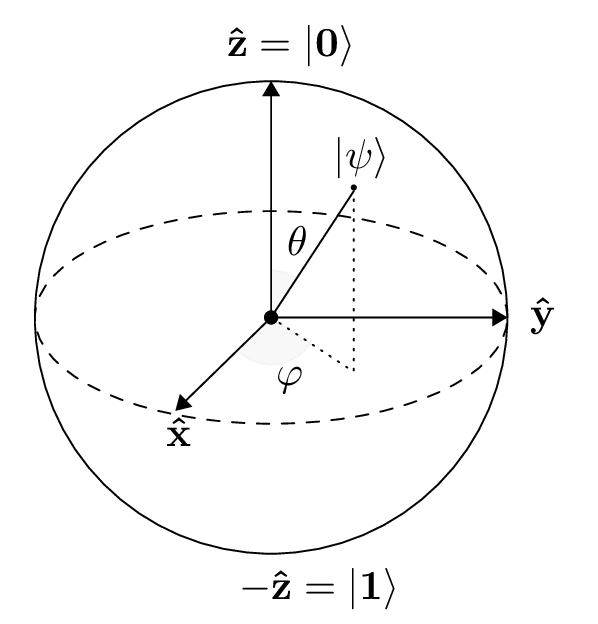
\includegraphics[width=0.5\linewidth]{img/img-ch2/bloch-sphere.png}
    \caption{The Bloch sphere representation of a qubit}
    \label{fig:bloch-sphere}
\end{figure}

\subsection{Quantum gates}
Postulates in \autoref{sec: measurements} and \autoref{sec: time evolution} highlighted the evolution of quantum states as well as their measurement. In quantum computing, time evolution operators are performed by quantum logic gates and measurements are done with respect to the computational basis. Next we will look at quantum gates. 

One-qubit quantum gates are formally described by $2 \times 2$ unitary transformations. 

\textbf{NOT gate}

The NOT gate, so-called X gate , is the quantum equivalent of the classical NOT gate. 
It is represented by the matrix
$$ X = \begin{bmatrix}
        0&1\\
        1&0\\
        \end{bmatrix} $$
It acts as:
\begin{align}
    \ket{0} &\longmapsto \ket{1} \\
    \ket{1} &\longmapsto \ket{0}
\end{align}
In other words, applied to a generic single-qubit state, the X gate swaps the amplitudes of the $\ket{0}$ and $\ket{1}$ components. 

Indeed, this gate corresponds to the Pauli X matrix. Coming back to the Bloch sphere, the X gate acts like a rotation of $\pi$ radians around the X axis of the Bloch sphere. We can generalize this behavior to obtain rotations of any angle around any axis of the Bloch sphere.

For the X axis we may define 
$$R_{X}(\theta)=e^{-i\frac{\theta}{2}X} = \begin{bmatrix}
        \cos \frac{\theta}{2}& -i \sin \frac{\theta}{2}\\
        -i \sin \frac{\theta}{2}& \cos \frac{\theta}{2}\\
        \end{bmatrix}$$
Analogously, for Y and Z axis:
\begin{align}
    R_{Y}(\theta)&=e^{-i\frac{\theta}{2}Y} = \begin{bmatrix}
        \cos \frac{\theta}{2}& - \sin \frac{\theta}{2}\\
        \sin \frac{\theta}{2}& \cos \frac{\theta}{2}\\
        \end{bmatrix}\\
    R_{Z}(\theta)&=e^{-i\frac{\theta}{2}Z} = \begin{bmatrix}
        e^{-i \frac{\theta}{2}}& 0\\
        0& e^{i \frac{\theta}{2}}\\
        \end{bmatrix}   
\end{align}

When $\theta=\pi$ the resulting matrices are known as \textbf{Pauli matrices}. Each of them define a quantum gate known as 
\begin{align}
    Y = R_{Y}(\pi)= \begin{bmatrix}
        0&-i\\
        i&0\\
        \end{bmatrix} \\
    Z = R_{Z}(\pi) = \begin{bmatrix}
        1&0\\
        0&-1\\
        \end{bmatrix} 
\end{align}

Another known gate coming from rotations of the Bloch sphere is the S gate which results from a $\frac{\theta}{2}$ rotation around the Z axis, known as \textbf{phase gate}:
$$ S = R_{Z}(\frac{\pi}{2})= \begin{bmatrix}
        1&0\\
        0&i\\
        \end{bmatrix} $$

\textbf{Hadamard gate}

Another remarkable gate is the Hadamard gate, denoted by H (which is not to be confused with the Hamiltonian also denoted by H). It is represented by the matrix
\begin{equation}
    H = \frac{1}{\sqrt{2}}\begin{bmatrix}
        1&1\\
        1&-1\\
        \end{bmatrix} 
\end{equation}

The Hadamard gate effect on the basis states $\ket{0}$ and $\ket{1}$ is 
\begin{align}
    \ket{0} &\longmapsto \frac{1}{\sqrt{2}}(\ket{0} + \ket{1}) \\
    \ket{1} &\longmapsto \frac{1}{\sqrt{2}}(\ket{0} - \ket{1})
\end{align}

Additionally, it is useful to keep in mind that
$$H = \frac{X+Z}{\sqrt{2}}$$

The role of the H gate is to create superposition of qubits.

For composite systems, we can guess that the tensor product will have a great importance again. The simplest way to build quantum gates on composite systems are tensor products of $2 \times 2$ unitary operators. In the case of two-qubit systems, the corresponding gates are $4 \times 4$ unitary operators constructed from the tensor product of two one-qubit quntum gates. Let $U_1$ and $U_2$ be one-qubit gates, the matrix of the gate $U_1 \otimes U_2$ is given by the tensor product of the matrices associated to $U_1$ and $U_2$:

\begin{align}
    U_1 \otimes U_2&=\begin{bmatrix}
        a_{11}&a_{12}\\
        a_{21}&a_{22}\\
        \end{bmatrix} 
    \otimes \begin{bmatrix}
        b_{11}&b_{12}\\
        b_{21}&b_{22}\\
        \end{bmatrix} 
    = \begin{bmatrix}
        a_{11} \begin{bmatrix}
        b_{11}&b_{12}\\
        b_{21}&b_{22}\\
        \end{bmatrix} &a_{12} \begin{bmatrix}
        b_{11}&b_{12}\\
        b_{21}&b_{22}\\
        \end{bmatrix} \\
        a_{21} \begin{bmatrix}
        b_{11}&b_{12}\\
        b_{21}&b_{22}\\
        \end{bmatrix} &a_{22} \begin{bmatrix}
        b_{11}&b_{12}\\
        b_{21}&b_{22}\\
        \end{bmatrix} \\
        \end{bmatrix} \\
    &= \begin{bmatrix}
        a_{11}b_{11}&a_{11}b_{12} &a_{12}b_{11}&a_{12}b_{12}\\
        a_{11}b_{21}&a_{11}b_{22}& a_{12}b_{21}&a_{12}b_{22}\\
        a_{21}b_{11}&a_{21}b_{12}& a_{22}b_{11}&a_{22}b_{12}\\
        a_{21}b_{21}&a_{21}b_{22}& a_{22}b_{21}&a_{22}b_{22}\\
        \end{bmatrix} 
\end{align}

By taking tensor products of one-qubit gates, we can only obtain operations that act on each qubit individually, but there are many unitary matrices that cannot be written as the tensor product of other matrices. A remarkable one is the controlled-NOT gate.

\vspace{5pt}
\textbf{CNOT gate}

The CNOT gate, known as controlled NOT gate is given by the unitary matrix
\begin{equation}
    CNOT = \begin{bmatrix}
        1&0&0&0\\
        0&1&0&0\\
        0&0&0&1\\
        0&0&1&0\\
    \end{bmatrix}
\end{equation}

It takes two input qubits, known as the control qubit and the target qubit. The state of the target qubit is changed, based  on the value of the control qubit. This is the principle of controlled gates. In particular, the CNOT gate, performs the NOT operation when the  control qubit is in state $\ket{1}$, otherwise, it remains unchanged. 

Next we will show how this gate acts on the elements of the two-qubit computational basis 

\begin{equation}
    CNOT \ket{00} = \ket{00},\quad  CNOT \ket{01} = \ket{01}, \quad CNOT \ket{10} = \ket{11}, \quad  CNOT \ket{11} = \ket{10}
\end{equation}

More generally, given an arbitrary qubit unitary operation denoted by $U$. A controlled $U$ operation is a two qubit transformation, again with a control and a target qubit. If the control qubit is set, then $U$ is applied to the target qubit, otherwise the target qubit is left alone.

The previously presented quantum gates are summarised at \autoref{tab: quantum gates}.

\begin{table}
    \centering
    \begin{tabular}{ccc}
    \toprule
        Gate     & Circuit representation    & Matrix \\
        \hline 
        \addlinespace
        X-Pauli (NOT) & \begin{quantikz} & \gate{X} & \qw\\ \end{quantikz} \egroup {& $\begin{bmatrix} 0&1\\1&0  \end{bmatrix}$\\
        Y-Pauli & \begin{quantikz} & \gate{Y} & \qw\\ \end{quantikz} \egroup {& $\begin{bmatrix} 0&-i\\i&0  \end{bmatrix}$\\
        Z-Pauli & \begin{quantikz} & \gate{Z} & \qw\\ \end{quantikz} \egroup {& $\begin{bmatrix} 1&0\\0&-1  \end{bmatrix}$\\
        Phase & \begin{quantikz} & \gate{S} & \qw\\ \end{quantikz} \egroup {& $\begin{bmatrix} 1&0\\0&i  \end{bmatrix}$\\
        Hadamard & \begin{quantikz} & \gate{H} & \qw\\ \end{quantikz} \egroup {& $\frac{1}{\sqrt{2}}\begin{bmatrix} 1&1\\1&-1  \end{bmatrix}$\\
        CNOT & \begin{quantikz} \lstick{} & \ctrl{1} & \qw\\ \lstick{} & \targ{} & \qw\\ \end{quantikz} \egroup {& $\begin{bmatrix} 1&0&0&0\\ 0&1&0&0\\ 0&0&0&1\\ 0&0&1&0\\\end{bmatrix}$\\
    \end{tabular}
    \caption{Summary table of useful quantum logic gates and their representations}
    \label{tab: quantum gates}
\end{table}

Departing from this overview of quantum gates we have the basis to build more complex gates and circuits.

\section{Open quantum systems}
As we have briefly mentioned in previous sections, the most widely treated and studied quantum systems are those called closed systems, which are the ones that only interact with themselves, isolated from the rest of the universe. By definition, it is a system which does not interchange information with another system. All the previous description of quantum mechanics was built in the realm of closed quantum systems. However, beyond theoretical level, closed quantum systems are not that relevant because no system can be completely isolated from its environment in the real world. Indeed, for this to happen, it would be needed a sort of ``infinite barrier'' around the system in question that cannot be recreated in an experimental environment. Therefore, since no quantum system is completely isolated from its surroundings, it is important to develop a theoretical framework for treating these interactions in order to obtain an accurate understanding of quantum systems. We have decided to introduce the notion of open quantum systems, a quantum mechanical system that interacts with an external quantum system, which is known as the environment or bath. We will analyze its evolution considering that it is not isolated from the rest of the universe and the mutual actions between the system and the environment. 


\begin{definicion}[Open quantum system]
    An open quantum system is a quantum mechanical system $S$, which is associated to a Hilbert space $\mathbb{H}_S$, that is interacting with another quantum system $E$: the environment, which is associated to a Hilbert space $\mathbb{H}_E$. Let's assume that $\dim (\mathbb{H}_S)=n$ and $\dim(\mathbb{H}_E)=n$. \\Therefore, $S$ is a subsystem of the total system $(S+E)$, whose corresponding Hilbert space is the tensor product $\mathbb{H}_T=\mathbb{H}_S \otimes \mathbb{H}_E$, that is $nm$-dimensional.
\end{definicion}

Traditionally, the time evolution of quantum systems has been described through a unitary transformation that connects the states of the system at two points in time. However, this description becomes excessively restrictive when attempting to analyze the time evolution of an open quantum system. To understand how the open quantum system that we have just defined evolves in time we will denote $H_s$ the open quantum system Hamiltonian, $H_e$ the environment Hamiltonian and $H_{se}$ the system-environment interaction Hamiltonian. Assuming that the entire open quantum system is a large closed system, its time evolution is governed by a unitary transformation generated by a global Hamiltonian given by
$$H = H_s \otimes I_e + I_s \otimes H_e + \alpha H_{se}$$
where $I_s$ and $I_e$ are the identity operators of the system and environment Hilbert spaces respectively, $\alpha$ is a coupling constant that depends on the interaction between the system and the environment. 

Since the system $S+E$ evolves according to a unitary time evolution operator $U(t,t_0)$, the density operator of the composite system at an initial time $t_0$ is described by a density matrix $\rho(t_0)$. The density operator at a time $t$ is given by $\rho(t)=U(t,t_0)\rho(t_0) U^{\dag}(t,t_0)$. The quantum states of the subsystems $S$ and $E$ at time $t$ are represented by their respective reduced density operators denoted by $\rho_S(t)$ and $\rho_E(t)$. These operators contain all the relevant statistical information for potential measurements performed on each subsystem. To obtain $\rho_S(t)$ and $\rho_E(t)$, it is needed to calculate the partial trace of $\rho(t)$ with respect to the degrees of freedom of $E$ and $S$, respectively.
\begin{align}
    \rho_S(t) &= \mathrm{Tr}_E(\rho(t)) \\
    \rho_E(t) &= \mathrm{Tr}_S(\rho(t))
\end{align}

\begin{definicion}[Partial trace]
    Let $X,Y$ be finite vector spaces of dimension $n$ and $m$ respectively. The partial trace over $Y$ is a linear operator defined as $\mathrm{Tr}_Y: \mathcal{L}(X \otimes Y) \longrightarrow \mathcal{X} $ such that
    $$\mathrm{Tr}_Y(T \otimes U) = \mathrm{Tr}(U) T \quad \forall T \in \mathcal{L}(X), \, \forall U \in \mathcal{L}(Y) $$

    Analogously, the partial trace over $X$ is $\mathrm{Tr}_X: \mathcal{L}(X \otimes Y) \longrightarrow \mathcal{Y} $ such that
    $$\mathrm{Tr}_X(T \otimes U) = \mathrm{Tr}(T) U \quad \forall T \in \mathcal{L}(X), \, \forall U \in \mathcal{L}(Y) $$
\end{definicion}

As the density operator of the environment is positive and normalized, it has a spectral decomposition in an orthonormal basis with non negative eigenvalues. Hence, 
$$\rho_E(t)=\sum_{v}\lambda_v \ket{v}\bra{v}$$
where $\lambda_v$ are the eigenvalues and $\left\lbrace \ket{v}\right \rbrace $ are the corresponding orthonormal eigenvectors.

We can express the reduced density operator of $S$ performing the partial trace in the orthonormal basis of the environment eigenstates:
\begin{align}
    \rho_s(t)&=\mathrm{Tr}_E\left[(U(t,t_0) \rho(t_0) U^{\dag}(t,t_0)\right] \\
    &= \sum_{\mu} \braket{\mu | U(t,t_0) \rho(t_0) U^{\dag}(t,t_0) | \mu}
\end{align}

We will assume, as is customary, that at the initial time the density operator of the closed system $S+E$ is separable, that is $\rho(t_0) = \rho_S(t_0)\otimes \rho_E(t_0)$ and that the reduced density operator $\rho_E(t_0)$ is equal to a certain fixed value $\rho_{E,0}$ regardless of the value of $t_0$. Then, the initial state of the total system at $t_0$ would be $\rho(t_0) = \rho_S(t_0)\otimes \rho_{E,0}$. It follows that
\begin{align}
    \rho_S(t)&=\mathrm{Tr}_E\left[ U(t,t_0) \rho_S(t_0) \otimes \rho_{E,0} U^{\dag}(t,t_0) \right] \\
    &= \sum_{\mu v} K_{\mu v}(t, t_0) \rho_S(t_0) K_{\mu v}^{\dag}(t, t_0) 
\end{align}
where $K_{\mu v}(t,t_0)$ are operators acting on the Hilbert space of $S$, known as Kraus operators. They are given by 
$$K_{\mu v}(t,t_0) = \sqrt{\lambda_v}\braket{\mu | U(t,t_0) | v}$$

The equation defining the system in terms of Kraus operators is called the Kraus Operator Sum representation. 

Just as the Schrödinger equation describes how pure states evolve in time, the equation governing the temporal evolution of the density operator of a closed quantum system is the Liouville-von Neumann equation
\begin{equation}
    \frac{d \rho(t)}{d t} = -\frac{i}{\hbar}\left[ H(t), \rho(t)\right]
\end{equation}
where $H(t)$ represents the Hamiltonian of the system, the square brackets denote the commutator of the operators enclosed within and $\hbar$ is Planck's constant.

By the Taylor expansion around $t=0$ we have:
$$\rho(dt)=\rho(0) + \frac{d \rho (t)}{dt}|_{0} + O(dt^2)$$
Using the Kraus Operator Sum representation,
$$\rho(dt)=\sum_{\alpha} K_{\alpha}(dt) \rho(0) K_{\alpha}^{\dag}(dt)$$
where we have collected the $\mu v$ indices into a single index $\alpha$.

It can be shown (\cite{lidar2019lecture}) that the reduced density operator of $S$ fulfills the evolution equation 
\begin{equation}
    \frac{d \rho_S(t)}{d t}|_{0} = -\frac{i}{\hbar}\left[ H_S, \rho_S(0)\right] + \sum_{j=1}^{n^2-1}\gamma_j \left[ L_j\rho_S(0) L_j^{\dag} - \frac{1}{2}(L_j^{\dag}L_j, \rho_S(0) )\right]
\end{equation}
This result is valid as a short time expansion near $t=0$. Making the assumption that the previous equation is valid for all times $t>0$, which is essentially the Markovian limit, that states that there is no memory in the evolution, as manifested by the fact that the evolution resets every $dt$. This takes us to

\begin{equation}
    \frac{d \rho_S(t)}{d t} = -\frac{i}{\hbar}\left[ H_S(t), \rho_S(t)\right] + \sum_{j=1}^{n^2-1}\gamma_j(t) \left[ L_j(t) \rho_S(t) L_j^{\dag}(t) - \frac{1}{2}(L_j^{\dag}(t)L_j(t), \rho_S(t) )\right] = \mathcal{L}\rho
\end{equation}
 
where $H_S(t)$ is an operator playing the role of the Hamiltonian for $S$ but which also contain information about the environment $E$, $n$ is the dimension of the Hilbert space of $S$, $\left\lbrace \gamma_j(t) \right\rbrace_{j=1}^{n^2-1}$ is a set of nonnegative functions with dimensions of frequency, $\left\lbrace L_j(t) \right\rbrace_{j=1}^{n^2-1}$ is a set of dimensionless operators known as Lindblad operators or quantum jump operators, and the braces denote the anticonmmutator of the operators enclosed within. This equation is known as \textbf{Gorini-Kossakowski-Sudarshan-Lindblad} (GKSL) equation or simply as the \textbf{Lindblad master equation}. The first term on the right-hand of the equation represents the unitary evolution of the system, whereas the second term describes the dissipative aspect of the dynamics. In the typical case where the time evolution operator $U(t,t_0)$ is invariant under temporal translations, that is $U(t+ \tau, t_0 + \tau) =U(t,t_0), \, \forall t,t_0,\tau \in\mathbb{R}$, then $H(t)$, $L_j(t)$ and $\gamma_j(t)$ become constants, resulting in a time-independent Lindblad master equation.

The generator of the evolution, $\mathcal{L}$ is called the Lindblandian. The form of the dissipative part of the Lindblandian, is 
$$\mathcal{L}_D[\cdot] = \sum_{j=1}^{n^2-1}\gamma_j \left[ L_j\rho_S(0) L_j^{\dag} - \frac{1}{2}(L_j^{\dag}L_j, \rho_S(0) )\right], \quad \gamma_j >0$$

We can now define the decoherence phenomena. Decoherence is what happens when $\mathcal{L}_D \neq 0$. This means that the evolution of the density matrix is governed not only by the Liouville-von Neumann component $\frac{-i}{\hbar}[H, \cdot]$ responsible for the unitary evolution, but also by the dissipator, which gives rise to non-unitary evolution. 

The formal solution of the Lindblad equation 
$\frac{d \rho_S(t)}{d t} = \mathcal{L}\rho_S$ is $$\rho_S(t) = e^{\mathcal{L}t} \rho_S(0) \equiv \Lambda(t) \rho_S(0) $$

For a certain $t$, the application $\Lambda(t)$ is called a dynamic application. If we consider the family of maps over time generated by the GKSL equation we obtain a one-parameter family $\left\lbrace \Lambda(t) : \, t \geq 0 \right \rbrace$ of dynamic applications that satisfy the following properties:
\begin{enumerate}
    \item Identity operator: $\Lambda(0)=\mathbb{1}$
    \item Closed under multiplication: since we are assuming a Markovian behaviour, it follows the Markov property,
    $$\Lambda(t_1)\Lambda(t_2) = \Lambda(t_1+t_2), \quad t_1, t_2 \geq 0$$
    which is also the property of the semigroup.
    \item Associative: $(\Lambda(t_1)\Lambda(t_2))\Lambda(t_3) = \Lambda(t_1)(\Lambda(t_2)\Lambda(t_3))$
\end{enumerate}

Therefore, the family of one-parameter dynamic applications generated by the GKSL equation form a \textbf{quantum dynamical semigroup}. For providing the definition of this structure, first we need to introduce the following notions.

Let $X$ be a Banach space and let $f \in X^*$. We denote $\varphi_f: X \longrightarrow \mathbb{R}$ the linear functional $\varphi_f(x)=\braket{f,x}$. As $f$ runs through $X^*$ we obtain a collection $\left \lbrace \varphi \right\rbrace_{f \in X^*}$ of maps from $X$ into $\mathbb{R}$. We define a new topology on the set $X$:

\begin{definicion}[Weak topology]
    The weak topology $\sigma(X, X^*)$ on $X$ is the coarsest topology associated to the collection $\left \lbrace \varphi_f \right\rbrace_{f \in X^*}$
\end{definicion}

We are now going to define a topology on $X^*$ called the \textbf{weak$^*$ topology} and denoted by $\sigma(X^*,X)$. For every $x\in X$ consider the linear functional $\varphi_x: X^* \longrightarrow \mathbb{R}$ defined by $f \longmapsto \varphi_x(f)=\braket{f,x}$. As $x$ runs through $X$ we obtain a collection $\left\lbrace \varphi _x \right\rbrace_{x\in X}$ of maps from $X^*$ into $\mathbb{R}$.

\begin{definicion}[Weak$^*$ topology]
    The weak$^*$ topology $\sigma(X^*,X)$ is the coarsest topology on $X^*$ associated to the collection $\left\lbrace \varphi _x \right\rbrace_{x\in X}$
\end{definicion}

Next, we will characterise the notion of convergence in these topologies.
\begin{definicion}
    \begin{itemize}
        \item A sequence $\left\lbrace x_n \right \rbrace$ in $X$ converges to $x$ in the weak topology $\sigma(X,X^*)$,
        $$x_n \rightharpoonup x $$
        if and only if $$\braket{f,x_n} \longrightarrow \braket{f,x}\, \forall f \in X^*$$

        \item A sequence $\left\lbrace f_n \right\rbrace$ in $X^*$ converges to $f$ in the weak$^*$ topology $\sigma(X^*,X)$, 
        $$f_n \stackrel{*}{\rightharpoonup} f $$
        if and only if 
        $$\braket{f_n,x}\longrightarrow \braket{f,x},\, \forall x \in X$$
    \end{itemize}
\end{definicion}

It is worth pointing out that if $f_n \stackrel{*}{\rightharpoonup} f $ in $\sigma(X^*,X)$ and $x_n \rightharpoonup x$ in $\sigma(X,X^*)$, in general, one cannot conclude that $\braket{f_n,x_n} \longrightarrow \braket{f,x}$. 

Now, we will briefly go through some concepts of the theory of Banach algebras, a large are in functional analysis. We will assume that the underlying field of scalars $\mathbb{K}$ is the field of complex numbers $\mathbb{C}$. An algebra over $\mathbb{C}$ is a vector space $\mathcal{A}$ over $\mathbb{C}$ that also has a multiplication defined on it that makes $\mathcal{A}$ into a ring such that if $\alpha \in \mathbb{C}$ and $a,b \in \mathcal{A}$, $\alpha(ab)=(\alpha a)b = a(\alpha b)$

\begin{definicion}[Banach algebra]
    A Banach algebra is an algebra $\mathcal{A}$ over $\mathbb{C}$ that has a norm $||\cdot||$ relative to which $\mathcal{A}$ is a Banach space and such that for all $a,b \in \mathcal{A}$,
    $$||ab|| \leq ||a||\,||b||$$
\end{definicion}

A $C^*$-algebra is a particular type of Banach algebra that is intimately connected with the theory of operators on a Hilbert space.

If $\mathcal{A}$ is a Banach algebra, an \textbf{involution} is a map 
\begin{align}
    \mathcal{A} &\longrightarrow \mathcal{A} \\
    a &\longmapsto a^*
\end{align}
such that the following properties hold for $a,b \in \mathcal{A},\, \alpha \in \mathbb{C}$:
\begin{enumerate}
    \item $(a^*)^*=a$
    \item $(ab)^* = b^*a^*$
    \item $(\alpha a +b)^* = \bar{\alpha}a^* +b^*$
\end{enumerate}

\begin{definicion}[$C^*$-algebra]
    A $C^*$-algebra is a Banach algebra $\mathcal{A}$ with an involution such that for every $a$ in $\mathcal{A}$,
    $$ ||a^*a||=||a||^2$$
\end{definicion}

\begin{definicion}[Von-Neumann algebra]
    A Von-Neumann algebra $\mathcal{A}$ is a $C^*$-algebra of the bounded operators $\mathcal{B}(\mathbb{H})$ in a Hilbert space that is closed under the weak$^*$ topology and contains the identity $I \in \mathcal{B}(\mathbb{H})$
\end{definicion}
 
Lastly, we can define the concept of quantum dynamical semigroups.
\begin{definicion}[Dynamic semigroup]
    Let $\mathcal{A}$ be a von-Neumann algebra. A dynamic semigroup is defined as a one-parameter family of applications $\Phi_t: \mathcal{A} \longrightarrow \mathcal{A}$ with the following properties:
    \begin{enumerate}
        \item $\Phi_t$ is positive for all $t\geq 0$
        \item $\Phi_t(I)=I$
        \item $\Phi_s \cdot \Phi_t = \Phi_{s+t}$
        \item $\Phi_t(X) \stackrel{*}{\rightharpoonup} X$ when $t \longrightarrow 0$
        \item $\Phi_t$ is weakly$^*$ continuous operator in $\mathcal{A}$
    \end{enumerate}
\end{definicion}

\section{Closing remarks}
The revolution in the world of physics in the 1920s led to the creation of quantum mechanics, an indispensable part of science ever since. Quantum computing emerges from this field, as proposed by Richard Feynman, in order to understand and simulate it.

Another major triumph of the 20th century was computer science. Within a century, there were proposals for the Turing machine, the construction of the first computers, and hardware development. In 1965, Gordon Moore declared that computational power would double at a constant cost every two years, meaning that the number of transistors in a microprocessor would double every two years. However, there is a limit to this due to quantum effects interfering with the operation of increasingly smaller electronic components. To overcome this barrier, one possible solution is to shift the computing paradigm: quantum computing.

In essence, quantum computing is the union of both branches, but after its invention and theoretical formulation: What are its possibilities? Quantum computing surpasses classical computing for some specialized tasks. The potential applications of quantum computing are still to be determined as it does not provide efficient solutions to all problems. However, this does not mean that quantum computing is an illusion or mere theory. Quantum algorithms have been developed, such as the famous Grover's Algorithm (for searching an unstructured search space) and Shor's Algorithm (for factorizing a number). The field of quantum information theory has been created, encompassing quantum computing, cryptography, and quantum communication. Furthermore, progress has been made in the theory of quantum error correction to protect data integrity.

On the other hand, companies are in a race to build quantum computers and have made many tools available to researchers and developers to program quantum algorithms and run them on their computers, such as IBM Quantum Composer and Quantum Lab, IBM's Qiskit, Google Quantum AI's Cirq, PennyLane, D-Wave's Leap, and many more.

Quantum computing will coexist with classical computing; it is not a paradigm that will replace the other, as both have their strengths. It is a burgeoning new field with challenges and questions to investigate, engaging physicists, engineers, and mathematicians in research groups and companies today.

\endinput
%--------------------------------------------------------------------
% FIN DEL CAPÍTULO. 
%--------------------------------------------------------------------

% !TeX root = ../tfg.tex
% !TeX encoding = utf8

\chapter{Quantum Machine Learning}\label{ch:3-QML}


Quantum machine learning is the field that involves the application of machine learning techniques, with the distinctive aspect that quantum computing is integrated at some phase of the process. As seen in \autoref{ch:1-MathematicalFundamentalsML} the basic ingredients of a machine learning setup consists on a computational model to tackle the problem, lots of data to ``feed'' the model and a algorithm of optimization of the configuration of the model so that our model learns from the training data. Therefore, quantum machine learning can vary from the use of a quantum computer in some part of the model, the use of data generated by some quantum process to the use of a quantum computer to process quantum-generated data to achieve improved insights.


In an attempt to further specify the broad world of quantum machine learning we are going to follow the categorization proposed by Schuld and Petruccione in \cite{schuld2021machine}. There are four intersections on the possible ways to combine quantum computing and machine learning depending on the generation of the data (  by a quantum system (Q) or a classical system (C)) and the information processing device (being a quantum (Q) or a classical (C) device).
\begin{itemize}
    \item The CC intersection covers classical data being processed classically, which is the conventional approach to machine learning, but in this contexts, it concerns the classical machine learning techniques that are based on ideas from quantum computing. So there is no actual quantum computing involved in this approach, just some inspiration.
    \item The QC intersection considers classical machine learning algorithms that operate on quantum data. It can be understood whether as classical machine learning methods that are run on data generated by quantum processes or as the application of classical machine learning to quantum computing. 
    \item The kind of quantum machine learning that is referred on this thesis and in the bibliography taken into consideration is the intersection CQ: classical data being processed by a quantum computer. These machine learning techniques are implemented within a quantum computer that is fed classical data. Quantum computing is involved in the model or in the training of the machine learning techniques.
    \item Ultimately, there is the QQ category that works on quantum data being processed by a quantum computer. As in the CQ intersection, quantum computing may be involved in the models or in the training processes, but in this case, the quantum data needs to come from measuring a quantum system (in a physical experiment or in a simulation of it run on a quantum computer) such as \cite{Perrier_QDataSet_Quantum_Datasets_2021} and \cite{schatzki2021entangled} proposals. QQ can be viewed as an extension of CQ and it is definitely a promising area but the required technologies and research on this intersection are still scarce.
\end{itemize}

\begin{figure}
    \centering
    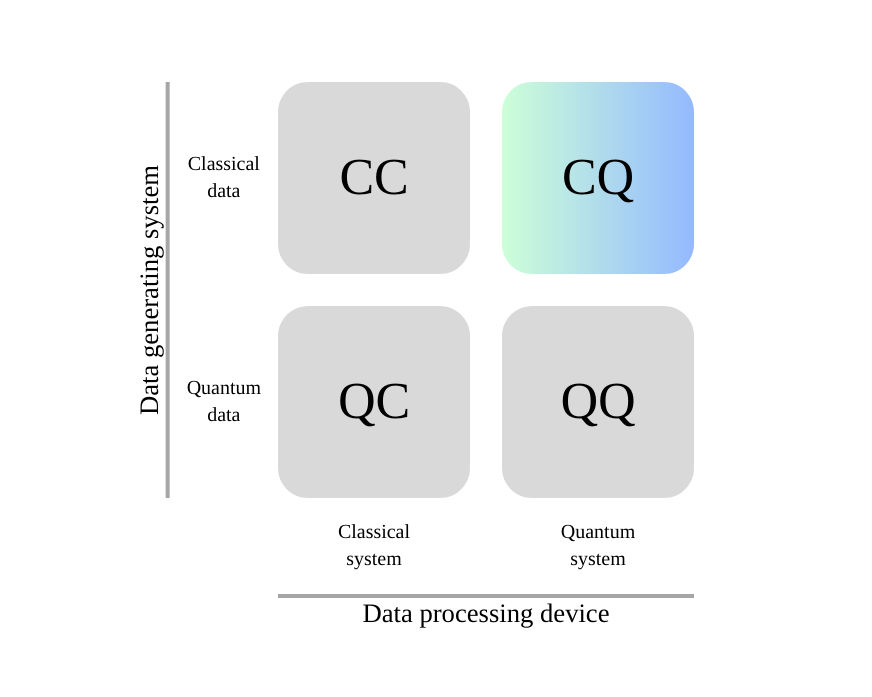
\includegraphics[width=\linewidth]{img/img-ch3/four_intersections_ML-QC.png}
    \caption{The four approaches to combine quantum computing and machine learning, categorized according to the nature of the data and the system used}
    \label{fig:four-intersections}
\end{figure}

In this thesis we will focus on CQ quantum machine learning, but within this category there is a broad range of possibilities. We will leave aside the proposals of  quantum algorithms that could speed up classical machine learning because they rely on a full error-corrected quantum computer that is currently beyond the limits of the state-of-the-art. Instead, we will dedicate to the study of fully quantum-oriented models that can be run on NISQ devices. \footnote{NISQ stands for noise intermediate-scale quantum computers, that are at our disposal now.} The goal is to use a quantum device as a machine learning model, not just as an alternative hardware to accelerate computation. This leads to new models and training algorithms derived from a quantum computational paradigm that require a the solid understanding of the intricacies of machine learning. Exploring the possibilities of NISQ computers and machine learning algorithms suitable to be executed on them will be a crucial field in the short and medium terms. It may bring us closer to the way for the first practical applications of quantum computing come to life. 

\section{Quantum support vector machines} \label{sec:QSVM}
Quantum support vector machines are a particular case of general support vector machines that rely on kernel methods in which we use quantum computers to map data into a space of quantum states. The kernel method, as seen in \autoref{subs:kernel-methods}, consists in mapping the data from its original space to a higher dimensional space known as feature space in which we wish our data could be separable by a hyperplane. In other words, by raising the dimensionality, the so called feature map can transform the problem into a linearly separable one. Quantum computing and kernel methods are based on a similar principle, a straightforward way to visualize it is presented in \autoref{fig:parallelism}. Both have mathematical frameworks in which information is mapped into and then processed in high-dimensional spaces to which we have only limited access. In kernel methods, the access to the feature space is facilitated though kernels (which are inner products of feature vectors). In quantum computing, access to the Hilbert space of quantum states is given by measurements, which can also be expressed through inner products of quantum states.

\begin{figure}
    \centering
    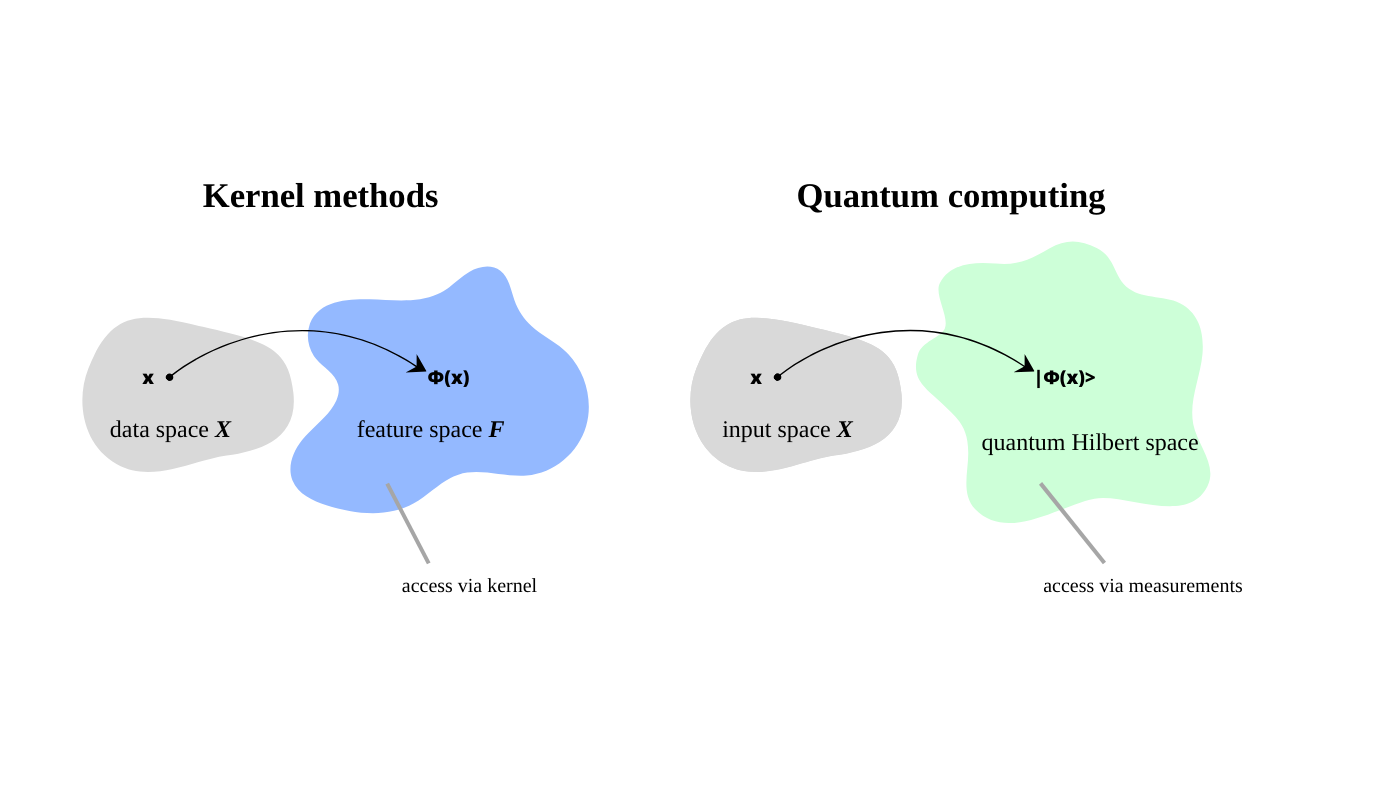
\includegraphics[width=\linewidth]{img/img-ch3/paralelism_KM-QC.png}
    \caption{Parallelism between the framework of kernel methods and the world of quantum computing. Illustration of own production inspired by \cite{schuld2021machine}.}
    \label{fig:parallelism}
\end{figure}


Therefore, we can view quantum support vector machine as ordinary support vector machines that rely on kernel methods where the feature space $\mathcal{F}$ is a certain space of quantum states. In order to train and use QSVM for classification, we will be able to operate as usual with classical SVM, except for the computation of the kernel function, which will require a quantum computer to
\begin{enumerate}
    \item Take as input two vectors in the original space of data, $\mathcal{X}$.
    \item Map each vector to a quantum state through a feature map, $\Phi$.
    \item Compute the inner product of the  quantum states and return it.
\end{enumerate}

Let's dive deeper into the mathematical framework that supports QSVM.
Kernel theory in feature space for machine learning uses linear algebra and functional analysis as tools to  pull data to a feature space for the sake of better discrimination of classes or simpler representation of data. 

\subsection{Feature map}\label{subsec: feature map}
Feature maps play an important role in machine learning, since they map any type of input data into a higher dimensional space with a well-defined metric. 

Essentially feature maps are just circuits that are parametrized exclusively by the original (classical) data and thus prepare a quantum state that depends only on that data. Consider a data embedding circuit $\Phi$ that depends on some classical data $x \in \mathcal{X}$. For each input $x \in \mathcal{X}$, we will have a circuit $\Phi(x)$ such that the output of the feature map will be the quantum state $\varphi(x)=\Phi(x) \ket 0$. 

%\textcolor{blue}{From the quantum physics perspective $x \longrightarrow \ket{\varphi(x)}$ would be a valid feature map, nevertheless it's not a good choice of feature map to then be able to apply comfortably the kernel theory since \textbf{quantum models are not linear in the Hilbert space of the quantum system}\footnote{ WHY? I can't really see why}. Instead the quantum feature map of choice will be $x \longrightarrow \phi(x) = \ket{\varphi(x)} \bra{\varphi(x)}$.}

\begin{definicion}[Feature map]
    Given a Hilbert space $\mathcal{F}$, called the feature space, an input set $\mathcal{X}$ and $x \in \mathcal{X}$ a sample from the input set. A feature map is a map $\Phi : \mathcal{X \longrightarrow \mathcal{F}}$ from inputs to vectors in the Hilbert space. The vectors $\Phi(x) \in \mathcal{F}$ are called feature vectors.      
\end{definicion}

By definition of inner product, every feature map gives rise to a kernel.

\begin{teorema}\label{th:feature map->kernel}
    Given a feature map $\Phi: \mathcal{X} \longrightarrow \mathcal{F}$. The inner product defined in the feature space of two feature vectors (obtained via the feature map) defines a kernel. 
    $$\kappa(x,y)=\left< \Phi(x), \Phi(y) \right>_{\mathcal{F}}$$
\end{teorema}
\begin{proof}
    We shall see that the previously defined kernel is a semi-definite function by showing that its Gram matrix is positive definite. 
    Let $c_i,c_j \in \mathbb{C}$ and $x_i \in \mathcal{X}$ for $i,j \subseteq \left\lbrace1,...M\right\rbrace$ with $M \geq 2$
    \begin{equation*}
        \sum_{i,j=1}^M c_i c_j \kappa(x_i,x_j) = \left< \sum_{i=1}^M c_i \Phi(x_i) , \sum_{j=1}^M c_j \Phi(x_j) \right> = ||\sum_{i=1}^M c_i \Phi(x_i) ||^2 \geq 0 
    \end{equation*}
\end{proof}


\subsection{Reproducing kernel Hilbert spaces}
Kernel theory gives rise to the reproducing kernel Hilbert space (RKHS), a rather abstract concept yet useful in order to understand the importance of kernels for machine learning, as their connection to linear models in feature space. 

So far, we are dealing with two Hilbert spaces: the Hilbert space of the quantum system and the feature space $\mathcal{F}$ that contains the embedded data by the feature map. Now we will build another feature space for the quantum kernel, derived directly from the kernel. This feature space is a Hilbert space $\mathcal{R}$ of functions and due to its definition it is called the reproducing kernel Hilbert space.

\begin{definicion}[RKHS]
    Let $\mathcal{X}$ be a non-empty input set and $\mathcal{R}$ a Hilbert space of functions $f:\mathcal{X} \longrightarrow \mathbb{K}$ that map inputs to real numbers. Let $\left< \cdot, \cdot \right>$ be the inner product on $\mathcal{R}$. \\$\mathcal{R}$ is a reproducing kernel Hilbert space if every point evaluation is a continuous functional $ F: f \longrightarrow f(x) \quad \forall x \in \mathcal{X}$. This condition is equivalent to the condition that there exists a function $\kappa : \mathcal{X} \times \mathcal{X} \longrightarrow \mathbb{K}$ for which $\left< f, \kappa(x,\cdot)\right> = f(x)$, with $\kappa(x,\cdot) \in \mathcal{R}, \forall f \in \mathcal{H}, x \in \mathcal{X}$. 
    
    The function $\kappa$ is the unique reproducing kernel of $\mathcal{R}$. 
    
    % A Reproducing Kernel Hilbert Space (RKHS) is a Hilbert space $\mathcal{H}$ of functions $f:\mathcal{X} \longrightarrow \mathbb{K}$ with a reproducing kernel $\kappa : \mathcal{X} \times \mathcal{X}  \longrightarrow \mathbb{K}$ where $\kappa(x,\cdot)\in \mathcal{H}$ and $f(x)=\left< \kappa(x,y), f \right> \quad \forall y \in \mathcal{X}$.
\end{definicion}

To understand it better let's consider a kernel function of two variables $\kappa(x,y)$. For $n$ points we fix one of the variables to have $\kappa(x_1,y)$, $\kappa(x_2,y)$,..., $\kappa(x_n,y)$. These are $n$ functions of the variable $y$. RKHS is a function space which is the set of all possible linear combinations of these functions:
\begin{equation}
    \mathcal{R} = \left\lbrace f(\cdot)=\sum_{i=1}^{n} \alpha \kappa(x_i, \cdot) \quad \forall y \in \mathcal{X} \right\rbrace
\end{equation}

As we have just seen, the functions that belong to the RKHS are linear combinations of its elementary kernel functions $\kappa(x,\cdot)$ where one variable is fixed in a possible data sample $x \in \mathcal{X}$. This kernel $\kappa(x,\cdot)$ assign a distance measure to every data point. Computing $\kappa(x,y)$ gives us the distance between the two points $x,y \in \mathcal{X}$. 
Therefore, the functions $ f(y)=\sum_{i=1}^{n} \alpha \kappa(x_i, y) \in \mathcal{R}$ are linear combinations of data similarities. 

For example, using one of the most widely used kernels, a Gaussian kernel $$\kappa(x,y)=\exp{\frac{|| x-y || }{2 \sigma^2}}$$ the functions $f \in \mathcal{R}$ are linear combinations of Gaussians centred in each data point. The kernel regulates the ``smoothness'' of the functions in $\mathcal{R}$ by changing the variance of the Gaussian. 

In order to calculate the inner product of two functions in RKHS $f, g \in \mathcal{R}$, since every function in RKHS can be written as a linear combination, $f=\sum_{i=1}^n \alpha_i \kappa(x_i, \cdot)$ and $g= \sum_{j=1}^n \beta_j \kappa(y_j, \cdot)$, 
\begin{align}\label{eq:inner-product-RKHS}
    \left< f, g\right> 
    &= \left< \sum_{i=1}^n \alpha_i \kappa(x_i,\cdot), \sum_{j=1}^n \beta_j \kappa(y_j, \cdot) \right> \\
    &\stackrel{(1)}{=}  \left< \sum_{i=1}^n \alpha_i \kappa(x_i,\cdot), \sum_{j=1}^n \beta_j \kappa(\cdot, y_j) \right> \\
    &= \sum_{i=1}^n \sum_{j=1}^n \alpha_i \beta_j \kappa(x_i, y_j)  
\end{align}

where $(1)$ uses that the kernel is symmetric. 
Indeed this is a well-defined inner product:
\begin{enumerate}
    \item It is symmetric, because so it is $\kappa$
    $$\left<g,f\right>= \sum_{j=1}^n \sum_{i=1}^n \beta_j \alpha_i \kappa(y_j, x_i) = \left<f,g\right>$$
    \item It is bilinear

    Observe,
    $$\left<f,g \right>= \sum_{j=1}^n \beta_j \sum_{i=1}^n \alpha_i \kappa(x_i, y_j) = \sum_{j=1}^n \beta_j f(y_j) $$

    Then we have,
    \begin{align}
        \left< f_1 + f_2, g\right> &= \sum_{j=1}^n \beta_j (f_1(y_j) + f_2(y_j)) \\
        &= \sum_{j=1}^n \beta_j f_1(y_j) + \sum_{j=1}^n \beta_j f_2(y_j) \\
        &= \left< f_1, g \right> + \left< f_2, g\right>
    \end{align}

    Similarly, we can show that $\left<f, g_1 + g_2 \right> = \left< f,g_1\right> + \left< f,g_2 \right>$
    \item It is positive semi-definite, since the kernel $\kappa$ is positive semi-definite. Next we will see that in fact, it is strictly positive definite. It is the last characteristic missing to prove it is an valid inner product.
\end{enumerate}

The name RKHS consists on several parts, let's analyse its meaning:
\begin{itemize}
    \item ``Reproducing'' because of the reproducing property of this space.
    
    We consider $g \in \mathcal{R}$ a kernel in RKHS space. In other words, we take $g$ to have only one component ${g(x)=\sum_{j=1}^n \beta_j \kappa(x_i,x) = \beta \kappa(x,x)}$. We take $\beta=1$ to have $g(x)=\kappa (x,x) $. 
    
    We also consider $f \in \mathcal{R}$ as  $f=\sum_{i=1}^n \alpha_i \kappa(x_i,y)$. According to \autoref{eq:inner-product-RKHS}, the inner product of $f,g \in \mathcal{R}$ is:
    \begin{align}
        \left< f(x), g(x)\right> &= \left< f, \kappa_x(\cdot) \right> \\
        &= \left< \sum_{i=1}^n \alpha_i \kappa(x_i,x) , \kappa (x,x) \right> \\
        &= \sum_{i=1}^n \alpha_i \kappa(x_i,x) = f(x)
    \end{align}
    This means that the function f is reproduced from the inner product of that function with one of the kernels of the space. In conclusion, the reproducing property is $$\left< f, \kappa(x,\cdot)\right> = f(x) $$ with $\kappa(x,\cdot), f \in \mathcal{R}, x \in \mathcal{X}$. 

    It is worth pointing out the special case
    \begin{equation*}\label{eq:special case reproducing property}
        \left< \kappa(x, \cdot), \kappa(x, \cdot) \right> = \kappa(x,x)
    \end{equation*}
    
    \item ``Kernel'' because of the kernels associated to RKHS as priorly stated.
    
    \item ``Hilbert space'': because $\mathcal{R}$ is a complete prehilbertian space. 
    
    We need to check that $\left<\cdot, \cdot\right>$ is strictly positive definite:
    \begin{equation*}
        |f(x)|^2 \stackrel{(1)}{=} |\left< \kappa(x, \cdot), f\right>|^2 \stackrel{(2)}{\leq} \left< \kappa(x, \cdot), \kappa(x, \cdot) \right> \cdot \left< f, f \right> = \kappa(x,x) \left<f, f \right>
    \end{equation*}
    where we use
    \begin{enumerate}
        \item The reproducing property
        \item The special case of the reproducing property \autoref{eq:special case reproducing property}
    \end{enumerate}
    It follows that $\left<f,f\right> = 0$ if $f=0$ is the identically null function. Therefore $\left<\cdot ,\cdot \right>$ is strictly positive definite and we can claim that it is an inner product.
    Now, we consider the norm $$||f|| = \sqrt{\left<f,f\right>}$$ $\mathcal{R}$ includes the limit points of sequences that converge in that norm. That makes it a complete space.
\end{itemize}


Since a feature map induces a kernel and a kernel gives rise to a reproducing kernel Hilbert space, we can construct a unique reproducing kernel Hilbert space for any given feature map.

\begin{teorema}\label{th:kernel->RKHS}
    Let $\Phi:\mathcal{X} \longrightarrow \mathcal{F}$ be a feature map over an input set $\mathcal{X}$, giving rise to a complex kernel $\kappa(x,y)=\left<\Phi(x),\Phi(y) \right>_{\mathcal{F}}$. The corresponding reproducing kernel Hilbert space has the form 
    \begin{equation} \label{eq:Rk}
        \mathcal{R}_{\kappa} = \left\lbrace f: \mathcal{X} \longrightarrow \mathbb{K} \,|\, f(x) = \left< w, \Phi(x) \right>_{\mathcal{F}}, \quad \forall x\in \mathcal{X}, w \in \mathcal{F} \right\rbrace
    \end{equation}
\end{teorema}

\begin{definicion}[Linear models]
    Let $\mathcal{X}$ be a data domain and $\Phi: \mathcal{X} \longrightarrow \mathcal{F}$ a feature map. A linear model in $\mathcal{F}$ is a function that maps every $x \in \mathcal{X}$ to the inner product of its feature map $\Phi(x)$ and a certain vector in the feature space $w \in \mathcal{F}$. Formally,
    $$f(x) = \left< \Phi(x), w \right>_{\mathcal{F}}$$ with $w \in \mathcal{F}$.
\end{definicion}

\begin{teorema}
    Deterministic quantum models are linear models in data-encoding feature space. Let $f(x)=\mathrm{tr} \left\lbrace \rho \mathcal{M} \right\rbrace$ be a quantum model and $\Phi: \mathcal{X} \longrightarrow \mathcal{F}$ the feature map $\Phi(x)=\rho(x) \in \mathcal{F}$. The quantum model $f$ is a linear model in $\mathcal{F}$.
\end{teorema}

This was the missing point to understand the relevance of the reproducing kernel Hilbert space: the functions living in the RKHS are the quantum model functions, which we have just stated that are linear models. Thus, the RKHS is equivalent to the space of linear models derived from the reproducing kernel. To conclude, the kernel essentially defines the class of functions that the linear model can express and, as a result, learn.

As seen in \autoref{eq:Rk}, the functions $\left< w, \cdot \right>$ in the RKHS $\mathcal{R}_{\kappa}$  associated with feature map $\Phi$ can be interpreted as linear models for which $w \in \mathcal{F}$ defines a hyperplane in feature space. 

%\textcolor{green}{Include theorems 6.3 and 6.4 from \cite{schuld2021machine}?}

\subsection{Quantum kernels}

As anticipated in \autoref{subs:kernel-methods}, the relation between kernels and inner products has a great importance in machine learning since they are a means of computation in the feature space without having to deal with the feature vectors $\Phi(x)$. Therefore, the classifier can be inferred from a kernel function that encodes the scalar product between the new features.

Now, let the feature space be the Hilbert space of the quantum system. We want to find out the kernel associated to that system, which we will call the quantum kernel. The methodology of work would be to encode some input $x \in  \mathcal{X}$ into a quantum state $\ket{\Phi(x)} \in \mathcal{F}$ described by a vector in the feature Hilbert space. This ``input-encoding'' procedure corresponds to what we have defined as \textbf{feature map} $\Phi: \mathcal{X} \longrightarrow \mathcal{F}$. There are different input encoding techniques in quantum machine learning, we discuss more on them in this section. According to \autoref{th:feature map->kernel} the feature map $\Phi$ induces a kernel $\kappa$:
$$ \kappa(x,y)=\left< \Phi(x), \Phi(y) \right>_{\mathcal{F}} \quad \forall x,y \in \mathcal{X}$$
As stated by \autoref{th:kernel->RKHS} the kernel $\kappa$ induces a RKHS $\mathcal{R}_{\kappa}$ (where $\kappa$ is the reproducing kernel). The functions in $\mathcal{R}_{\kappa}$ are the inner products of the feature maps of the input data and a vector $\ket{w} \in \mathcal{F}$ which defines a linear model $$ f(x, w) = \braket{w | \Phi(x)} $$
Note that we use Dirac brackets $\braket{\cdot | \cdot}$ instead of the inner product $\left< \cdot , \cdot \right>$ to denote the inner produts in a quantum Hilbert space.

It is worth pointing out that the idea of interpreting $ x \longrightarrow \ket{\Phi(x)}$ is the starting point that allows us to make use of the entire framework of kernel theory. 

\begin{definicion}[Quantum kernel]
    Given $\Phi$ a feature map over an input domain $\mathcal{X}$. A quantum kernel is the Hilbert-Schmidt inner product between two feature vectors $\varphi(x), \varphi(y)$ where $x,y \in \mathcal{X}$:
    \begin{equation}
        \kappa(x,y) = \mathrm{tr} \left\lbrace \varphi(y), \varphi(x) \right\rbrace = |\braket{\Phi(y)|\Phi(x)}|^2
    \end{equation}
\end{definicion}


The quantum kernel previously defined is indeed a kernel because it is a positive definite function. We can see that it is a product of the complex kernel $\kappa(x,y) = \braket{\Phi(y)|\Phi(x)}$ and its complex conjugate $\kappa(x,y)^*=\braket{\Phi(x)|\Phi(y)}$. It is needed to check that the complex conjugate of a kernel is a kernel itself. Given $x_i \in \mathcal{X}, \quad i=1,...,n$ and $c_i \in \mathbf{C}$,
\begin{align}
    \sum_{i,j=1}^n c_i c_j^*(\kappa(x_i,x_j))^* &= \sum_{i,j=1} c_i c_j^* \left< \Phi(x_i), \Phi(x_j)\right> \\
    &= (\sum_{i=1}^n c_i \bra{\Phi(x_i)}) \cdot (\sum_{i=1}^n c_i^* \ket{\Phi(x_i)}) \\
    &= || \sum_{i=1}^n c_i^* \ket{\Phi(x_i)} ||^2 \geq 0
\end{align}
So the complex conjugate of a kernel is also positive definite.

Lastly, the product of two kernels is known to be a kernel.


To bring to life the definition of quantum kernel, we need to dive into different examples of data encoding feature maps, its feature-embedding circuits and kernels they give rise to.

\begin{enumerate}
    \item \textbf{Basis encoding.} The data encoding feature map of basis encoding maps a $n$ bit binary string $x = (b_1,...b_n) $ with $b_i \in \left\lbrace 0,1\right\rbrace, \quad i=1,...,n$ to a computational basis state in a $n$-qubit system, which in turn corresponds to a standard basis vector $ \ket{i_x}$ , with $i_x$ being the integer representation of the bitstring), in a $2^n$-dimensional Hilbert feature space. This feature map is given by $$\Phi: x \in \left\lbrace 0,1 \right\rbrace^n \longrightarrow \ket{i_x} $$

    Basically this feature map maps each data input to a state from an orthonormal basis.

    The associated quantum kernel is the Kronecker delta
    $$\kappa(x,y) = \left< \Phi(x), \Phi(y) \right>_{\mathcal{F}} = \braket{i_x|i_y} \stackrel{(1)}{=} \delta_{x,y}$$

    in $(1)$ we observe we are computing the inner product in a quantum Hilbert space (hence the Dirac notation)  of orthonormal states by definition of the feature map. 
    
    This kernel is a binary similarity measure on the input space that is only nonzero for two identical inputs, thus really strict and hardly ever a good choice of data encoding for quantum machine learning tasks.
    
    \item \textbf{Amplitude encoding. } The data encoding feature map of amplitude encoding maps each input vector into the amplitudes of a quantum state with respect to a fixed basis, the orthonormal computational basis. Let $\mathbf{x}=(x_0,...,x_{N-1} ) \in \mathbb{R}^N $ be a input vector of dimension $N=2^n$. This encoding technique maps it to the amplitudes of a $n$-qubit state $\ket{\psi_{\mathbf{x}}}$.
    \begin{equation*}
        \Phi: \mathbf{x}\in \mathbb{R}^N \longrightarrow \ket{\psi_{\mathbf{x}}} = \frac{1}{\sqrt{\sum_{i}x_i^2}} \sum_{i=0}^{N-1} x_i \ket{i}
    \end{equation*}

    where $\ket{i}$ denotes the i-th computational basis state. 
    It is worth pointing out that we have included a normalization factor to make sure that the output is, indeed, a quantum state. This definition of amplitude encoding doesn't work for the null vector.
    
    Amplitude encoding offers an important benefit in terms of spatial efficiency compared to basis encoding. Using basis encoding, in a $n$-qubit system we can only codify strings of $n$ classical bits, whereas using amplitude encoding we can store vectors of dimension $2^n$. 

    The associated quantum kernel is:
    $$\kappa(\mathbf{x},\mathrm{y})=\left< \Phi(\mathbf{x}),\Phi(\mathrm{y}) \right> = \braket{\psi_{\mathbf{x}} | \psi_{\mathrm{y}}} = \mathbf{x}^{T} \mathrm{y}$$

    \item \textbf{Copies of quantum states. } Similarly done as in amplitude encoding, this data encoding technique maps each input vector $\mathbf{x} \in \mathbb{R}^N$ to $d$ copies of an amplitude encoded quantum state.
    \begin{equation*}
        \Phi: \mathbf{x}\in \mathbb{R}^N \longrightarrow \ket{\psi_{\mathbf{x}}} \otimes ... \otimes \ket{\psi_{\mathbf{x}}}
    \end{equation*}
    The associated quantum kernel is known as homogeneus polynomial kernel
    $$\kappa(\mathbf{x},\mathrm{y})=\left< \Phi(\mathbf{x}),\Phi(\mathrm{y}) \right> = \braket{\psi_{\mathbf{x}} | \psi_{\mathrm{y}}} \otimes ... \otimes \braket{\psi_{\mathbf{x}} | \psi_{\mathrm{y}}} = (\mathbf{x}^{T} \mathrm{y})^d$$

\end{enumerate}


% From practical book Finally we observe that it is equivalent to computing the probability of measuring all zeros after preparing the state $\Phi^*(x) \Phi(y) \ket{0}$. Therefore, the kernel operation results to be 
%\begin{equation}
 %   \kappa(x,y) = |\braket{0| \Phi^*(x) \Phi(y) | 0} |^2
%\end{equation}

% From practical book To sum up, the implementation of a quantum kernel function consists on taking a feature map that returns a circuit $\Phi(x)$ for any input $x \in \mathcal{X}$, then preparing the state $\Phi^*(x) \Phi(y) \ket{0}$ for the pair of vector $x,y$ on which we want to compute the kernel and finally returning the probability of measuring zero on all the qubits.


Next, we will go through one of the main achievements of classical kernel theory: the representer theorem. It states that the function $f$ from the RKHS which minimises the cost function can always be expressed as a weighted sum of the kernel between $x$ and the training data. 

\begin{teorema}[Representer theorem]
    Given $\mathcal{X}$ an input domain, $\mathcal{Y}$ an output domain. Let $\kappa$ be $\kappa: \mathcal{X} \times \mathcal{Y} \longrightarrow \mathbb{R}$ a kernel, with a corresponding reproducing kernel Hilbert space $\mathcal{R}_{\kappa}$, $\mathcal{D}$ a training data set consisting of $M$ data pairs $\mathcal{D} = \left\lbrace (x_1,y_1),...,(x_M,y_M) \in \mathcal{X} \times \mathcal{Y} \right\rbrace$. Assume a cost function $C$ that quantifies the quality of a model by comparing predicted outputs $f(x_i)$ with targets $y_i$ and consider a strictly monotonic increasing regularisation function $g: \interval[open right]{0}{\infty} \longrightarrow \mathbb{R}$.

    Then any function $f_{opt} \in \mathcal{R}_{\kappa}$ that minimises the cost function $C$
    \begin{equation*}
        f_{opt} \in \mathrm{argmin}_{f \in \mathcal{R}_{\kappa}} \left\lbrace \hat{R_L}(f) + g(||f||_{\mathcal{R}_{\kappa}}) \right\rbrace
    \end{equation*}
    
    admits a representation as
    \begin{equation}\label{eq:representer theorem}
        f_{opt}(x)=\sum_{i=1}^M \alpha_i \kappa(x, x_i) 
    \end{equation}
    where $\alpha_i \in \mathbb{R}, \forall 1 \leq i \leq M$.
\end{teorema}

Any model function $f \in \mathcal{R}_{\kappa}$ can be expressed,
\begin{equation}
    f(x)=\sum_{i=1}^{\infty}\mu_i \kappa(x,x_i) \label{eq:f infinite sum} \tag{$*$}
\end{equation}
since $f$ lives in the RKHS, a function space made up of linear combination of kernel functions.

Being $f$ a model function that minimises the cost function  $C$, by the representer theorem, can be written as
\begin{equation}
    f_{opt}(x)=\sum_{i=1}^M \alpha_i \kappa(x, x_i) \label{eq: f finite sum} \tag{$**$}
\end{equation}

The great step that the representer theorem allows us to take is passing from the model function in the feature space expressed by an infinite sum \eqref{eq:f infinite sum}, to its expression formulated in terms of kernels over the finite $M$ training inputs \eqref{eq: f finite sum}. Thus, even if we are trying to solve an optimization problem in an infinite dimensional space $\mathcal{R}_{\kappa}$ containing linear combinations of kernels centered on arbitrary $x_i$, then the solution lies in the span of the $M$ kernels centered on the $x_i$. This constrains the difficulty of the optimisation since it is just needed to solve the convex optimisation problem (there is only one global minimum) of finding the parameters $\alpha_i$, instead of explicitly optimising over an infinite dimensional RKHS. It follows from the fact that optimising over the RKHS of the quantum kernel is equivalent to optimising over the space of quantum models.


\begin{proof}
    Consider the subspace spanned by $K_M =\left \lbrace \kappa(x_i, \cdot) \right\rbrace_{i = 1}^{M}$. We will denote it as $\mathcal{Y}=\mathrm{span}\left\lbrace K_m \right\rbrace$. Assume we project $f \in \mathcal{R}_{\kappa}$ onto $\mathcal{Y}$ with the orthogonal projection ${P_{\mathcal{Y}}: \mathbb{H} \longrightarrow \mathcal{Y}}$.

    By the orthogonal projection theorem, \autoref{th:orthogonal projection theorem}, the function $f$ can be decomposed into $f_{\parallel} = P_{\mathcal{Y}}(f)$ and $f_{\perp} = P_{\mathcal{Y}^{\perp}}(f)$ and we have 
    \begin{equation}\label{eq:inequality orthogonal projection}
        ||f||_{\mathcal{R}_{\kappa}}^2 = ||f_{\parallel}||_{\mathcal{R}_{\kappa}}^2 + ||f_{\perp}||_{\mathcal{R}_{\kappa}}^2 \geq ||f_{\parallel}||_{\mathcal{R}_{\kappa}}^2
    \end{equation}
    
    This implies that $||f||_{\mathcal{R}_{\kappa}}$ is minimized if $f \in \mathcal{Y}$.

    Additionally, by the reproducing property of the RKHS $\mathcal{R}_{\kappa}$ we have for each $i=1,...,M$
    \begin{align}
        f(x_i)=\left< f, \kappa(x_i, \cdot) \right>_{\mathcal{R}_{\kappa}} &\stackrel{(1)}{=} \left< f_{\parallel}, \kappa(x_i, \cdot) \right>_{\mathcal{R}_{\kappa}} + \left< f_{\perp}, \kappa(x_i, \cdot) \right>_{\mathcal{R}_{\kappa}} \\
        &\stackrel{(2)}{=} \left< f_{\parallel}, \kappa(x_i, \cdot) \right>_{\mathcal{R}_{\kappa}} = f_{\parallel}(x_i)
    \end{align}

    where we use
    \begin{enumerate}
        \item the orthogonal decomposition of $f$ and the sesquilinear property of the inner product,
        \item the orthogonal component has zero inner product with the basis of the subspace.
    \end{enumerate}

    Therefore, 
    \begin{equation} 
        \hat{R_L}(f) = \frac{1}{M}\sum_{i=1}^M L(x_i, y_i, f(x_i)) =\frac{1}{M}\sum_{i=1}^M L(x_i, y_i, f_{\parallel}(x_i)) = \hat{R_L}(f_{\parallel}) \label{eq:R_L f and fparallel} 
    \end{equation}

     By virtue of \autoref{eq:inequality orthogonal projection} and equation \eqref{eq:R_L f and fparallel}, we can say that

     \begin{equation}
         \mathrm{min}_{f \in \mathcal{R}_{\kappa}} \left\lbrace \hat{R_L}(f) + g(||f||_{\mathcal{R}_{\kappa}}) \right\rbrace = 
         \mathrm{min}_{f \in \mathcal{R}_{\kappa}} \left\lbrace \hat{R_L}(f_{\parallel}) + g(||f_{\parallel}||_{\mathcal{R}_{\kappa}}) \right\rbrace 
     \end{equation}

    Which means this minimization depends only on the component of $f$ lying in the subspace $\mathcal{Y}$, consequently we can present the function $f_{opt}$ (solution of the optimization) to lie in the space as a linear combination of the basis vectors $\left \lbrace \kappa(x_i, \cdot) \right\rbrace_{i = 1}^{M}$ as stated in \eqref{eq: f finite sum}.
    
\end{proof}


\section{Quantum Neural Networks}
The subject of this section are quantum neural networks (QNN), the family of quantum machine learning models that together with quantum support vector machines form the most popular part of QML. 

Recovering the classification of quantum machine learning \autoref{fig:four-intersections}, quantum neural networks are part of the CQ intersection. Nevertheless, unlike quantum support vector machines, which are a particular case of a classical machine learning method; quantum neural networks are not a particular case although they are inspired by the operating procedure of classical neural networks. Over the literature on this topic, there are different conceptions on what is referred as quantum neural networks. Here we will focus on quantum neural networks in the form of parameterized quantum circuits.

Analysing the workflow of classical neural networks, we can differenciate the following stages of the process:
\begin{enumerate}
    \item \textbf{Data pre-processing. } It comprises the transformations performed on the input data (classical). The goal is to remain with more valuable information, codified in quantifiable attributes in the domain of the problem. The transformations forming this stage range from cleaning, instance selection, normalization, one-hot encoding, data transformation to feature extraction and feature selection.

    \item \textbf{Data processing. } This stage in neural networks world refers to the flow of data through the layers of the neural network. The behaviour of this processing depends on some parameters, which are optimized during the training phase.

    \item \textbf{Data output. } It consists on returning the output of the neural network, which is the output obtained through the final layer. 
\end{enumerate}

Following this strategy, we can define an analogous quantum neural network
\begin{enumerate}
    \item \textbf{Data pre-processing. } As we are in CQ branch, we have classical data: numbers or arrays of numbers and we work with a quantum system, that works with quantum states. Thus, we need to embbed the classical data into the space of quantum states. We have already faced this task in \autoref{subsec: feature map}. Feature maps allow us to encode the classical input of a quantum neural network into a quantum state. Then, we can easily apply other well-known data pre-processing techniques such as normalization and scaling. 

    \item \textbf{Data processing. } Once working with quantum states that encode the classical input data according to a certain feature map, we have to process this ``quantum input''. We should discard replicating exactly the behaviour and structure of a classical neural network, given the difficulty to translate it to the current quantum hardware. Nevertheless, we can take as a valid idea from classical neural networks the application of some transformations that depend on some optimizable parameters. 

    We can define this stage as the application of a circuit that depends on some optimizable parameters. This circuit receives the name of variational form or ansatz. We can understand it as a template of parametrised and fixed quantum gates, which define the architecture of the circuit, just like the layer structure defines the architecture of a classical neural network, thus it remembers us of the classical approach. The optimization of the parameters can be by the minimization of a cost function, which adapts the gates and hence, the circuit.

    \item \textbf{Data output. } After the data processing stage we obtain a output quantum state, but we need to return classical output. As we are familiar with quantum computers, a measurement operation allows us to access the space of quantum states and retrieve the output. The choice of the measurement operation is up to our choice depending on the domain of the problem. 
\end{enumerate}

\begin{figure}
    \centering
    \begin{quantikz}
    \lstick{$\ket{0}^{\otimes n}$} & \gate{S(\vec{x})} \qwbundle[alternate]{}& \qwbundle[alternate]{} & \gate{W(\vec{\theta})} \qwbundle[alternate]{}& \qwbundle[alternate]{} & \meter{} \qwbundle[alternate]{}
    \end{quantikz}
    \caption{General schema of a QNN. \\
    A quantum neural network takes a classical input $\vec{x}$ and maps it to a quantum state $\ket{\Phi(x)}$ through a feature map $\Phi$. This corresponds to the data pre-preprocessing stage and it is depicted in the above circuit as the block $S(\vec{x})$. The state $\ket{\Phi(x)}$ goes through a parametrised block that we have called ``variational form'' and it is represented by the block $W(\vec{\theta})$. It corresponds to the data processing stage. Finally, the output of the quantum neural network is the result of a measurement operation on the output of the variational form.}
    \label{fig:Generic QNN schema}
\end{figure}

\autoref{fig:Generic QNN schema} depicts the strategy just proposed for quantum neural networks as a quantum circuit. It receives the name variational circuit and for us, it will be a synonym of quantum neural network. 

Since we are already familiar with feature maps, next we will be devoted to understanding variational circuits.

\subsection{Variational circuits}
Variational circuits have changed the research objective of quantum machine learning and what to pursue. Given the limitations of near-term quantum computing, instead of aiming at speedups for known models, it has risen a new model family whose usefulness was- and still is- unknown, as well as new research questions beyond the usual computational speedups questions. 

Essentially, variational circuits are quantum circuits that depend on some parameters. Now, if we remember the definition from \autoref{ch:1-MathematicalFundamentalsML}, a machine learning deterministic model is a function $f_{\theta}: \mathcal{X} \longrightarrow \mathcal{Y}$ that maps input data to an output domain and depends on some parameters $\theta$. We can intuit some analogy between variational circuits and deterministic machine learning models. In order to interpret a variational quantum circuit as a deterministic machine learning model, we apply a quantum circuit $U(x,\theta)$ to the initial state $\ket{0}$. This quantum circuit depends on both the input data $x$ and the parameters $\theta$. And then we consider the expectation of a measurement $\mathcal{M}$ as the output of the model. 

Formally, we can define a deterministic quantum model as follows,

\begin{definicion}[Deterministic quantum model] \label{def:deterministic quantum model}
    Let $\mathcal{X}$ be an input data domain, $U(x, \theta)$ a quantum circuit that depends on inputs $x\in \mathcal{X}$ and parameters $\theta \in \mathbb{R}^n$, $\mathcal{M}$ a self-adjoint operator representing a quantum observable. $\ket{\Phi(x, \theta)}$ denotes the state prepared by $U(x, \theta)$ to the initial state $\ket{0}$. The function $f_{\theta}: \mathcal{X} \longrightarrow \mathcal{Y}$ is defined as the expectation value of the observable $\mathcal{M}$ of the quantum system in the state $\ket{\phi(x, \theta)} $

    \begin{equation}
        f_{\theta}(x)= \braket{\mathcal{M}}_{x,\theta} = \braket{\Phi(x,\theta) | \mathcal{M} | \Phi(x, \theta)}
    \end{equation}

    This function $f_{\theta}$ defines a deterministic variational quantum model.
\end{definicion}

The previously considered circuit $U(x,\theta)$ consists of a data embedding block $S(x)$ that corresponds to the data pre-processing stage, followed by a parametrised block $W(\theta)$ that we have previously named variational form. This interpretation of a variational circuit as a deterministic machine learning model is represented by $\autoref{fig:Generic QNN schema}$.

Now, let's dive deeper into how a variational form can be implemented. Theoretically, a variational form can have any internal structure, however in the context of quantum neural networks, variational forms follow a layered structure that reminds us of the spirit of classical neural networks. Next we will show this idea more accurately.

For variational form block $W(\theta)$ of $N$ layers we would consider $N$ parameters $\theta_1, ..., \theta_N$. Each layer $i$ would be defined by a variational circuit $W_i$ that depends on the parameter $\theta_i$ followed by a fixed unitary gate $V_i$ independent of any parameters. The variational form is then formed by stacking these layers consecutively. Therefore, the variational form block is formulated as
\begin{equation}
    W(\theta)=\prod_{i=1}^N W_{i}(\theta_i) V_i
\end{equation}

\autoref{fig:variational form} represents the variational form that has been just described.
%\textcolor{green}{Include time evolution expression of the block?}

Analogously, the data embedding block $S(x)$ can also have a layered structure identical to the one proposed above considering $\left\lbrace x_i \right \rbrace_{i=1}^M$ inputs. Each layer consisting on $S_i$ gate that depends on the $i$-th input followed by a fixed unitary gate $T_i$:
\begin{equation}
    S(x)=\prod_{i=1}^M S_{i}(x_i) T_i
\end{equation}

 \begin{figure}
    \centering
    \begin{quantikz}
    \lstick{$\ket{S(x)}$} & \gate{W_1(\theta_1)} \qwbundle[alternate]{} & \gate{V_1} \qwbundle[alternate]{}& \gate{W_2(\theta_2)} \qwbundle[alternate]{}& \gate{V_2} \qwbundle[alternate]{}& \qwbundle[alternate]{}\quad ... \quad & \gate{W_N(\theta_N)} \qwbundle[alternate]{}& \gate{V_N} \qwbundle[alternate]{}
    \end{quantikz}
    \caption{A variational form of $N$ layers}
    \label{fig:variational form}
\end{figure}



\subsection{Measurements}
Measurements are the final building block of every quantum neural network architecture. QNN take a classical input $x \in \mathcal{X}$ that is then fed through a feature map. The resulting quantum state is transformed by a parametrised block $W(\theta)$ that depends on some parameters $\theta$ and to conclude, a classical output is obtained through a measurement operation.

As we know, a measurement $\mathcal{M}$ is a Hermitian operator, that is, a self-adjoint operator. We are working in the quantum state space $\mathbb{H}$ which is a separable Hilbert space (view postulate 1 \autoref{sec: postulates of QM}. Therefore, we are in the hypothesis to apply the Spectral Theorem \autoref{th:spectral theorem} that grants us the existance of a orthonormal basis in $\mathbb{H}$ composed of eigenvectors of $\mathcal{M}$.

%\textcolor{green}{In this context, is it used the functional analysis version (that requires compactness of the self-adjoint operator and separability of the Hilbert space) valid for infinite dimensional spaces or the linear algebra version only valid for finite dimensional spaces?}

We will continue using the following notation
\begin{enumerate}
    \item $\lambda_k$ is the k-th eigenvalue of $\mathcal{M}$ 
    \item $\ket{\mu_k^j}$ is the eigenvector associated to the k-th eigenvalue and j ranges from 1 to the geometric multiplicity of the corresponding eigenvalue.
    \item $\left \lbrace \ket{\mu_k^j} \right\rbrace_{j,k}$ is the set of eigenvectors of $\mathcal{M}$. 
\end{enumerate}

The measurement operator $\mathcal{M}$ has a diagonal matrix representation in terms of the orthonormal basis of eigenvectors $\left\lbrace \ket{\mu_k^j} \right\rbrace_{j,k}$, with the eigenvalues in the diagonal.
We can formulate this like
\begin{equation}
    \mathcal{M}=\sum_{k,j} \lambda_k \ket{\mu_k^j} \bra{\mu_k^j}
\end{equation}
since the outer product of two eigenvectors (which are orthonormal) is:
\begin{equation*}
    \ket{\mu_k} \bra{\mu_k} = 
    \begin{bmatrix}
    0 & & & &\\
    & \ddots & & &\\
    &  & 1_{kk} & &\\
    & & & \ddots &\\
    & & & & 0
  \end{bmatrix}
\end{equation*}

Given that $\left \lbrace \ket{\mu_k^j} \right\rbrace_{j,k}$ is a orthonormal basis of the quantum state space $\mathbb{H}$, any quantum state $\ket{\varphi}$ can be written as a linear combination of eigenvectors
\begin{equation}\label{eq:state as linear combination of eigenvectors}
    \ket{\varphi}= \sum_{k,j} \braket{\mu_k^j | \varphi} \ket{\mu_k^j}
\end{equation}

Combining all the above, we obtain that the expectation value of the measurement becomes
\begin{equation}
    \mathcal{M}=\sum_{k,j} |\braket{\mu_k^j|\varphi}|^2 \lambda_k
\end{equation}
which is a natural definition that agrees with the statistical expected value of the results obtained when we measure $\varphi$ according to $\mathcal{M}$ since the term $|\braket{\mu_k^j|\varphi}|^2$ is the probability of measuring $\lambda_k$. This expression can be further simplified as follows:

\begin{align}
    \mathcal{M} &= \sum_{k,j} |\braket{\mu_k^j|\varphi}|^2 \lambda_k = \sum_{k,j} \braket{\mu_k^j|\varphi} \braket{\mu_k^j|\varphi} \lambda_k \\
    &\stackrel{(1)}{=} \sum_{k,j} \braket{\mu_k^j|\varphi} \braket{\varphi | \mathcal{M} | \mu_k^j} \stackrel{(2)}{=} \braket{\varphi | \mathcal{M}\sum_{k,j} \braket{\mu_k^j | \varphi} | \mu_k^j } \\
    &= \braket{\varphi | \mathcal{M} | \varphi}
\end{align}

where we have used 
\begin{enumerate}
    \item the fact that $\lambda_k$ is a eigenvalue of $\mathcal{M}$: $\lambda_k \ket{\mu_k^j} = \mathcal{M}\ket{\mu_k^j}$,
    \item and expressing $\ket{\varphi}$ as a linear combination of the orthonormal basis formed by eigenvectors \eqref{eq:state as linear combination of eigenvectors}.
\end{enumerate}

Remembering our definition of quantum neural network \autoref{def:deterministic quantum model}, we have just obtained the expression for the output of the model:
\begin{equation}
    f_{\theta}(x) = \sum_{k,j} |\braket{\mu_k^j | \Phi(x,\theta)}|^2 \lambda_k
\end{equation}
where $\ket{\Phi(x, \theta)}$ denotes the state prepared by $U(x, \theta)$ to the initial state $\ket{0}$ and the term $|\braket{\mu_k^j | \Phi(x,\theta)}|^2$ is the probability of measuring $\lambda_k$. To ease the notation we will assume that the geometric multiplicity of each eigenvalue is 1 and denote the probability of measuring $\lambda_k$ as $p(\lambda_k)$. 
\begin{equation}
    f_{\theta}(x) = \sum_{k} \lambda_k p(\lambda_k)
\end{equation}

When we measure a single qubit in the computational basis, the coordinate matrix with respect to the computational basis of the Hermitian operator of the measurement could be
$$N = \begin{bmatrix}
0&0\\
0&1\\
\end{bmatrix}$$
or 
 $$ Z= \begin{bmatrix}
1&0\\
0&-1\\
\end{bmatrix}$$

Both of these operators represent the same observable but differ in the eigenvalues that they associate to the different possible outcomes. The first operator $N$ associates the eigenvalues $0$ to the state $\ket{0}$ and the eigenvalue $1$ to the state $\ket{1}$. The second operator $Z$ associates the eigenvalue $1$ to the state $\ket{0}$ and $-1$ to the state $\ket{1}$. Indeed we can realise that the operator $Z$ corresponds to the Pauli Z matrix, $Z=\sigma_Z$. 

Let's consider the following example: we are working with a 2-qubit system and we take the measurement as $\mathcal{M} = \sigma_Z$, which is valid because it is self-adjoint. 

The eigenvalues of $\sigma_Z$ are $\lambda_{+}=+1$ and $\lambda_{-}=-1$. The eigenvectors are $\mu_{+}$ and $\mu_{-}$ respectively.

\begin{equation}
    \mu_{+}=
    \begin{bmatrix}
    1\\
    0\\
    \end{bmatrix} = \ket{0} 
    \quad \quad
    \mu_{-}=
    \begin{bmatrix}
    0\\
    1\\
    \end{bmatrix} = \ket{1} 
\end{equation}

When $\ket{\Phi(x, \theta)}$ denotes the state prepared by $U(x, \theta)$ to the initial state $\ket{0}$, the model reads
\begin{equation}
    f_{\theta}(x)= 1\,|\braket{0|\Phi(x, \theta)}|^2 + (-1)\,|\braket{\Phi(x, \theta)}|^2 = p(0)-p(1)
\end{equation}

The expectation value $\braket{\mathcal{M}}$ when $\mathcal{M} = \sigma_Z$ of a single qubit measurement in the computational basis is a value in the range $ \interval{-1}{1}$. In practice, the expectation is estimated by rerunning an algorithm $s$ times to sample $S$ bits in $\left \lbrace -1, 1 \right\rbrace$, where $S$ is also known as the number of shots. The estimate is then computed as the average of the bits. 


Let's stop a moment and recap what we have gone through this section so far. We have defined quantum neural networks as a deterministic quantum model that takes a classical input, map it to a quantum state through a feature map, that is then transformed by a variational form that depends on some $\theta$ parameters to then perform a measurement. In this field, some argue if quantum neural networks is a well-deserved name for variational circuits, because the essence of classical neural networks is their multi-layer perceptron structure. There are some ways to interpret variational circuits in which they are truly similar to neural networks. The data encoding step does not have a clear equivalent in neural networks, but we can consider each amplitude of  $\ket{\Phi(x, \theta)}$ (denotes the state prepared by $S(x)$ to the initial state $\ket{0}$) as the value of an input neuron in the first layer of a neural network. Remembering the layered structure of the parametrised block $W(\theta)$, the gates used apply linear transformations on the feature vectors. Every such transformation can be viewed as a linear layer within a neural network. Some of this linear layers are fixed ($V_i$) and others are trainable ($W_i(\theta_i)$). Finally, the measurement corresponds to a non-linear layer with an absolute square activation that is followed by a final layer that linearly combines the absolute squares of the amplitudes with weights, which are the eigenvalues of the measurement operator.   

\begin{figure}
   \centering
   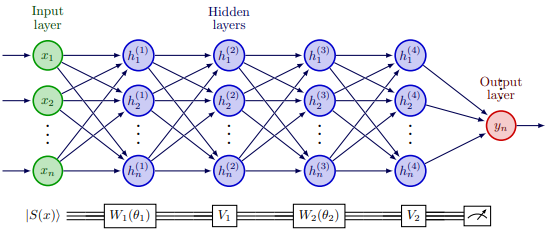
\includegraphics[width=\linewidth]{img/img-ch3/QNN_parallelism.png}
   \caption{Parallelism of a variational circuit with a classical neural network}
   \label{fig:QNN-parallelism}
\end{figure}

After all, we have a model and we can construct it theoretically. However, there is a missing ingredient that we haven not given the proper attention. We have mentioned several times about the optimizable parameter $\theta$, but up to know, we have not done anything about it. Moreover we are in the field of machine learning, so the step that we are missing is the training and that is where the optimization of $\theta$ parameter comes into the picture.


\subsection{Training a quantum neural network}
Training a quantum neural network consist on finding the parameters $\theta$ which minimise a data-dependent cost function. Consider a cost function $C(\theta)$ which relies on a model $f_{\theta}$ that depends on parameters $\theta$. The partial derivative of the cost with respect to $\mu \in \theta$ is
\begin{equation}
    \frac{\partial C}{\partial \mu} = \frac{\partial C}{\partial f_{\theta}} \frac{\partial f_{\theta}}{\partial \mu}
\end{equation}

In the training of variational circuits, $\frac{\partial C}{\partial f_{\theta}}$ is a classical computation, so it can be tackled by classical techniques and libraries. The problem comes when computing the partial derivative of $f_{\theta}$, which is the result of a quantum computation, with respect to $\mu \in \theta$ one of its variational parameters.

To unlock the potential of gradient-descent-based optimization strategies it is needed to have access to the gradients of quantum computations. By providing such partial derivatives, quantum computing can fit into hybrid machine learning pipelines without trouble and be trained.

First, we will go through a basic overview.

The model function of the quantum neural network is a scalar-valued function ${f_{\theta}: \mathbb{R}^N \longrightarrow \mathbb{R}}$. The gradient of the model is the vector of partial derivatives with respect to its parameters $\theta=\left\lbrace \theta_1,...,\theta_K\right\rbrace$,
\begin{equation}
    \nabla f_{\theta}= 
     \begin{bmatrix}
    \frac{\partial f_{\theta}}{\partial \theta_1}\\
    \vdots \\
    \frac{\partial f_{\theta}}{\partial \theta_K}\\
    \end{bmatrix}
\end{equation}

There are different approaches to evaluate the gradients of a numerical computation.
\begin{enumerate}
    \item \textbf{Numerical differentiation.} We can always approximate the partial derivative numerically using the finite-differences method. Next we will apply it to a quantum model $f_{\theta}$ that depends on a parameter $\mu \in \theta$:
    $$\frac{\partial f_{\theta}}{\partial \mu} \approx \frac{f_{\theta} - f_{\theta + \delta \theta}}{|| \delta \theta ||}$$
    where $\delta \theta$ is the parameter set in which $\mu$ has been exchanged by $\mu + \delta \mu$, with $\delta \mu$ an infinitesimal shift.
    
    This is a linear approximation of the model between two different points. In a context where each function evaluation can only be estimated with an error, the finite-difference method is problematic. For small partial derivatives, we need more precision for each function evaluation, so we need more shots to estimate $f_{\theta}$, in other words, more repetitions of the algorithm. In situations when the minimum has to be approximated closely, the optimisation landscape has many saddle points and there is a high variance of the measurements, numerical finite-differences methods are not really suitable. 

    \item \textbf{Automatic differentiation. } It is a programming paradigm in which the gradient is efficiently computed through the accumulation of intermediate derivatives, following the chain rule. A well known automatic differentiation technique is the backpropagation algorithm for the training of classical neural networks.
    
    Unfortunately, for $f_\theta$ it is not clear how this intermediate derivatives could be stored and reused inside of a quantum computation, since the intermediate quantum states cannot be measured without impacting the overall computation and backpropagated information cannot be shared because of the quantum no-cloning theorem.

    \item \textbf{Parameter shift rule.} It comes from the idea of computing a partial derivative of a quantum computation using quantum computation, this means using the same circuit in the quantum neural network, yet shifting the values of the optimizable parameters. To compute gradients of quantum expectation values with respect to one of the variational parameters, the paramether shift rule follows this strategy: first we derive an equation for $\frac{\partial f_{\theta}}{\partial \mu},\, \mu \in \theta$ as a linear combination of the same expectation but with the parameter ``shifted''. The parts of this equation can be evaluated on a quantum computer and consequently combined on a classical coprocessor. Like this, evaluating $\frac{\partial f_{\theta}}{\partial \mu}$ can often be done on a circuit architecture similar or identical to the one of $f_{\theta}$ and requires the  evaluation of the model a few times, generally two, at different points in the parameter space.

    \begin{definicion} [Parameter shift rule]
        Let $f_\mu = \braket{\mathcal{M}}_{\mu}$ be a quantum expectation value that depends on $\mu$ a classical parameter. A parameter shift rule is an identity of the form
        \begin{equation}
            \frac{\partial f_{\mu}}{\partial \mu} = \sum_{i} a_i f_{\mu + s_i}
        \end{equation}
        where $a_i, s_i \in \mathbb{R}$
    \end{definicion}

    A consideration is that the shifts $s_i$ are not necessarily small infinitesimal values. With this computation, the gradient is not approximated, it is exact, however in practice, a quantum computer can only estimate an expectation value and therefore the parameter shift rule lets us compute an estimation of the analytic gradient. In contrast with the finite difference method through which we can compute an estimation of the approximate gradient. 

    There would be no problem with chaining parameter shift rules to compute higher order derivatives such as the Hessian. 
    
\end{enumerate}

To conclude, on one hand we have found a valid method, the parameter shift method, to compute the partial derivatives of quantum computations, thus we can calculate $\frac{\partial f_{\theta}}{\partial \mu}$. On the other hand, $\frac{\partial C}{\partial f_{\theta}}$ is a classical computation, that can be tackled by classical techniques and libraries such as automatic differentiation. In consequence, we can compute the partial derivative of the cost with respect to $\mu \in \theta$, 
\begin{equation}
    \frac{\partial C}{\partial \mu} = \frac{\partial C}{\partial f_{\theta}} \frac{\partial f_{\theta}}{\partial \mu}
\end{equation}
And we are in conditions to be able to apply gradient-descent-based optimization strategies to train quantum neural networks.

So, we have seen how to build a quantum neural network, its structure and operations and then we have figured out how to train it. Everything is proceeding smoothly up to this point. However, quantum neural networks also pose some challenges when it comes to training them that we haven't come accross yet. It is concerning the situations in which the training gradients vanish, and thus, the training can no longer progress. This situation is known as \textbf{Barren plateaus}. 

A vanishing gradient means that with high probability the partial derivatives are close to zero in all their elements, Barren plateaus can be understood as areas in the landscape of the cost function in which the gradients become zero. In turn, the optimisation cannot proceed because the optimisation is slow and expensive. To resolve the small signal and avoid a random walk, high-precision measurements are needed, which are a problem when we are working with noisy near-term quantum computers.

There are different root causes for this phenomenon. They are observed when variational circuit architectures are highly expressive and Hilbert spaces large. To have an idea of what this means we can imagine we are moving over long distances in a very large space, the impact of an individual step towards the ultimate destination does not have a huge effect. Therefore, this derives into an important design principle of variational quantum models: to find a suitable, limited structure for the variational form which restricts training to the relevant subspace of the enormous Hilbert space.

The presence of barren plateaus has a stochastic nature, the high probability of the partial derivatives being zero derives from the statistical properties of partial derivatives. 


\subsection{Considerations on QNN's}

As a conclusion for this section, we will reflect on a series of ideas and concerns to take into consideration regarding quantum neural networks.

\begin{enumerate}
    \item A quantum neural network depends on a feature map, a variational form and a measurement operation. These are three choices we have to make when designing a variational circuit depending on the problem and the data we are dealing with. 

    \item The data is a really important part of any machine learning method. It is what feeds the quantum neural network. We should consider pre-processing techniques according to the nature of the data and the chosen feature map.

    \item The design of the variational form and the number of optimizable parameters it works with is a determining factor for the power of the quantum neural network. If the variational form uses too many parameters, we risk overfitting, while with very few parameters, we would be threatened by underfitting.
    
\end{enumerate}

\nocite{*}

\endinput
%--------------------------------------------------------------------
% FIN DEL CAPÍTULO. 
%--------------------------------------------------------------------

% !TeX root = ../tfg.tex
% !TeX encoding = utf8

\chapter{Case study: entanglement detection}\label{ch:4-Implementation}



To continue further with our study of quantum machine learning methods, we will approach a binary classification problem using quantum support vector machines and quantum neural networks. First, let's get introduced to the problem.

\section{Problem}
Our goal for this chapter involved delving into the state-of-the-art quantum computing frameworks to translate the methods from \autoref{ch:3-QML} from theory to practice. To do so, our chosen approach has been to tackle a machine learning problem. In order to continue with the discourse of this thesis, we picked up Feynman's initial proposal of simulating physics with computers and we have chosen the \textbf{quantum separability problem}. It addresses detection and classification of quantum entanglement, a fundamental feature of quantum mechanics presented in \autoref{sec:entanglement}. This problem is based on determining if a certain quantum state is entangled or not. There has been proposals of different criteria for dealing with the separability problem such as Bell's inequalities, the Peres-Horodecki positive partial transpose criterion (PPT) and entanglement witnesses (\cite{HORODECKI19961, guhne2009entanglement}). 

In particular, we will only focus on bipartite quantum systems, that is, systems composed of two distinct subsystems. The Hilbert space $\mathbb{H}$ associated with a bipartite quantum system is given by the tensor product $\mathbb{H}_A \otimes \mathbb{H}_B$ of the subsystems $A$ and $B$. Those subsystems may not necessarily be the $2$-dimensional Hilbert state space of qubits, but any $n$-dimensional Hilbert space. Our problem will be constrained to $\mathbb{H}=\mathbb{H}_A \otimes \mathbb{H}_B$, where $\dim (\mathbb{H}_A )= \dim (\mathbb{H}_B ) = 3 $. A quantum state is described by a density matrix: a positive semidefinite Hermitian matrix of trace one. Let's quickly remember the notion of entanglement: a state (that is, a density matrix) that cannot be written as a tensor product of quantum states of the subsystems. Now we can express the quantum separability problem in the terms we will work with. This problem consists in deciding whether a bipartite density matrix is entangled or separable. Formally, it can be defined as follows:

\begin{tcolorbox}[title=Quantum separability problem]

    Let $\mathbb{H} = \mathbb{H}_A \otimes \mathbb{H}_B$ be a bipartite quantum state space and $\rho$ be a density matrix acting on $\mathbb{H}$. The quantum separability problem is to determine if ${\rho \in S_{+}^{p} = \left \lbrace \rho \in \mathbb{C}^{p \times p}: \rho \geq 0,\, \mathrm{Tr}(\rho)=1  \right\rbrace}$ admits a decomposition of the form
    \begin{equation}
        \rho = \sum_{j}q_j \sigma_{A,j} \otimes \sigma_{B,j} \text{ such that } q_j\in \mathbb{R}^{+},\, \sum_{j}q_j =1
    \end{equation}
    where $\sigma_{A,j} \in S_{+}^{p_A}$, $\sigma_{B,j} \in S_{+}^{p_B}$ are density matrices acting on $\mathbb{H}_A$ and $\mathbb{H}_B$, respectively, and the variables $\left\lbrace q_j \right\rbrace$ form a probability distribution.

    If $\rho$ admits such a decomposition, then it is said to be separable, otherwise it is said to be entangled.
\end{tcolorbox}



In the case of pure states, the Schmidt decomposition \autoref{th:schmidt decomposition} is a valid tool for detecting entanglement. However, for mixed states, the separability problem has been proved to be NP-hard \cite{gurvits2003classical}. 

The starting point has been the papers \cite{casale2023large, urena2023entanglement}, in which the separability problem is taken as a binary classification task that is approached with classical support vector machines and deep neural networks, respectively. To be able to do so, \cite{casale2023large} provide an efficient Frank-Wolfe based algorithm to approximately seek the nearest separable bipartite density matrix, derive a systematic way for labeling density matrices as separable or entangled and generate a labeled dataset with thousands of separable and entangled density matrices of sizes $9 \times 9$ (for the case $\mathbb{H}=\mathbb{H}_A \otimes \mathbb{H}_B$, where $\dim (\mathbb{H}_A )= \dim (\mathbb{H}_B ) = 3 $) and $49 \times 49$ ($\mathbb{H}=\mathbb{H}_A \otimes \mathbb{H}_B$, where $\dim (\mathbb{H}_A )= \dim (\mathbb{H}_B ) = 7 $). Additionally, the code and data of this work had been released at \href{https://gitlab.lis-lab.fr/balthazar.casale/ML-Quant-Sep}{their gitlab repository}, which has allowed us to take a subset of their data and manipulate it to obtain the dataset we will work with. In this study, we will take a step towards the ``quantum'' direction: we will apply the quantum machine learning methods that we have introduced in this thesis to the quantum separability problem. 

\section{Dataset}

The dataset we have worked with in this case study comes from \cite{casale2023large} 6000 samples dataset of separable and entangled density matrices, released at \href{https://gitlab.lis-lab.fr/balthazar.casale/ML-Quant-Sep}{their gitlab repository}. The effort that stands out in their research is the creation of a well-labeled training dataset, specially for high-dimensional density matrices and the release of this data encouraging reproducibility and future work aimed at detecting quantum entanglement. Their approach is based on the positive partial transpose (PPT) criterion and optimal entanglement witness. Next, we will present these criteria for bipartite entanglement.

\subsection{The PPT criterion}

First, we will start with the partial transposition. If we have a state $\rho$ that acts on $\mathbb{H}_A \otimes \mathbb{H}_B$, we can write $\rho$ density matrix in a chosen product basis as 
\begin{equation}
    \rho = \sum_{i,j}^{p_A} \sum_{k,l}^{p_B} \rho_{ij, kl} \ket{i}\bra{j} \otimes \ket{k}\bra{l}
\end{equation}
Given this decomposition, the partial transposition of $\rho$ with respect to one subsystem (in this case B) is defined as 
\begin{align}
    \rho^{T_B} &=\sum_{i,j}^{p_A} \sum_{k,l}^{p_B} \rho_{ij,kl} \ket{i}\bra{j} \otimes ( \ket{k} \bra{l})^T \\
    &= \sum_{i,j}^{p_A} \sum_{k,l}^{p_B} \rho_{ik, kl} \ket{i}\bra{j} \otimes \ket{l} \bra{k} \\
    &= \sum_{i,j}^{p_A} \sum_{k,l}^{p_B} \rho_{ik, lk} \ket{i}\bra{j} \otimes \ket{k} \bra{l}
\end{align}

This definition becomes more apparent when representing the density matrix in the form of a block matrix:

\begin{equation}
    \rho = \begin{bmatrix}
        \rho_{1,1}& \cdots & \rho_{1,p_A}\\
        \vdots & & \vdots\\
        \rho_{p_A,1} & \cdots & \rho_{p_A,p_A}
        \end{bmatrix} 
\end{equation}
where the blocks $\rho_{i,j}$ are $p_B \times p_B$ matrices $\forall i,j =1, ..., p_A$.

Then, the partial transpose is
\begin{equation}
    \rho^{T_B} = \begin{bmatrix}
        \rho_{1,1}^T& \cdots & \rho_{1,p_A}^T\\
        \vdots & & \vdots\\
        \rho_{p_A,1}^T & \cdots & \rho_{p_A,p_A}^T
        \end{bmatrix} 
\end{equation}

Similarly, we can define $\rho^{T_A}$ by exchanging $i$ and $j$ instead of $k$ and $l$. 

A density matrix $\rho$ has a positive partial transpose (or the matrix is PPT) if its partial transposition has no negative eigenvalues, thus it is positive semidefinite: $\rho^{T_B}\geq 0$. If a matrix is not PPT, we call it NPPT. 

\begin{teorema}[PPT Criterion]
    Let $\rho$ be a bipartite separable state. Then $\rho$ is PPT. 
\end{teorema}
\begin{proof}
    The PPT criterion follows directly from the definition of separability. If $\rho$ is a bipartite separable state, then 
    \begin{equation}
        \rho = \sum_{j}q_j \sigma_{A,j} \otimes \sigma_{B,j} 
    \end{equation}
    and we have $\rho^{T_B} = \sum_j q_j \sigma_{A,j} \otimes (\sigma_{B,j})^T$

    Since the transposition operation preserves eigenvalues, the spectrum of $(\sigma_{B,j})^T$ is the same as the spectrum of $\sigma_{B,j}$, therefore $(\sigma_{B,j})^T$ is positive semidefinite.  Consequently, the partial transposition $\rho^{T_B}$ is also positive semidefinite.
\end{proof}

For a given density matrix, this criterion guarantees us that if we can calculate its partial transpose and find a negative eigenvalue, then the state is entangled. The PPT criterion is a necessary condition, so it is natural to ask: is the PPT criterion sufficient for separability? That is, $\rho^{T_B} \geq 0$ implies separability?

\begin{teorema}[Horodecki Theorem]
    If $\rho$ is a bipartite density matrix such that $p_A=2$ and $p_B = 2$ or $p_B=3$, then $\rho^{T_B} \geq 0$ implies that $\rho$ is separable. In other dimensions this is not the case.
\end{teorema}

In $2 \times 2$ and $2 \times 3$ systems the PPT criterion is a necessary and sufficient condition for separability. When working with the separability problem in these dimensions from a machine learning approach, the PPT criterion is enough to label as separable or entangled the training density matrix set. However, in other dimensions there might be non-separable density matrices fulfilling the PPT condition. Note that PPT states contain separable and entangled states, while NPPT states are all entangled. Therefore, using the PPT criterion to label the dataset in these cases leads to a partial problem: being PPT or not, which is a different task from quantum separability and not really interesting. 

According to the PPT criterion, we can classify quantum states in the following classes:
\begin{itemize}
    \item \textbf{Separable}: density matrices that are separable fulfill the PPT criterion. In $2 \times 2$ and $2 \times 3$ all matrices that satisfy the PPT condition are separable.
    \item \textbf{PPT entangled}: density matrices that are entangled and fulfill the PPT condition. This class exists in systems of dimension different than $2 \times 2$ and $2 \times 3$ .
    \item \textbf{NPPT entangled}: density matrices which do not fulfill the PPT condition, that is, matrices whose partial transpose matrix has a negative eigenvalue and thus, are entangled. In $2 \times 2$ and $2 \times 3$ all the entangled states are matrices that do not satisfy the PPT condition.
\end{itemize}

The dataset includes separable, PPT entangled and NPPT entangled density matrices, each class stored in a file. The generation of PPT entangled density matrices is the great contribution of \cite{casale2023large}, providing a practical and efficient method that relies on the notion of entanglement witness.

\subsection{Methodology to obtain the dataset}
Working with the code and data released by \cite{casale2023large}, we took the following steps to create the dataset we will work with:
\begin{enumerate}
    \item The density matrices for separable and entangled states were stored in files. From them we read:
    \begin{itemize}
        \item $100$ separable density matrices, labeled $0$, and generated an array of separable density matrices
        \item $100$ entangled density matrices, labeled $1$. For one dataset, we fixed a $0.5$ PPT ratio, which means that we took $50\%$ of the entangled class to be PPT entangled density matrices and the remaining $50\%$ NPPT entangled states. For the other dataset, we took a PPT ratio of $1.0$, that is, all the entangled matrices were entangled and fulfilling the PPT condition. There is no presence of NPPT matrices in this dataset.
    \end{itemize}
    \item Both arrays were stacked to create a $200$ samples training dataset of bipartite $9 \times 9$ complex density matrices of a $3 \times 3$ system. 
    \item We transformed the array of complex density matrices (with shape $(200,9,9)$ into a real-valued vector of $200$ samples and $80$ attributes. This operation is based on the decomposition into the generalised Gell-Mann basis and provided in the repository of their paper.
    \item Finally, we exported the array containing our training set into a \textit{.csv} file. The training dataset with PPT ratio $0.5$ is stored in \textit{x\_train\_05.csv}. The dataset with PPT ratio $1.0$ corresponds with the file \textit{x\_train\_1.csv}.
\end{enumerate}

The process for creating the test set was analogous: we read the density matrices for separable and entangled states from the test files. In this case we took 100 samples of each type: $100$ samples of separable states, $100$ PPT entangled density matrices and $100$ NPPT entangled states. Resulting in a $300$ samples test set.

Our aim was to reproduce the conditions under which the paper \cite{casale2023large} works to be able to obtain comparable results. We took the reduced version of the training set composed by $200$ samples that they consider in the Appendix E.3. Their study is performed considering different PPT ratios, while we have constrained our research under the specific PPT ratios of $0.5$ and $1.0$. On the other hand, the test set used in the paper was composed of $3000$ samples, $1000$ samples per type (SEP, PPT-ent, NPPT-ent). Due to the long executing times of current quantum machine learning methods, we decided to work with a reduced version of the test set made of $300$ samples, $100$ samples per type. As a final consideration, we have not used data augmentation. 



\section{Implementation}

We approached the implementation part of this work using a Jupyter notebook, powered by Python, and hosted on Google Colab. This choice of tools not only facilitated the smooth implementation of the project but also offered the advantage of accessibility, collaboration and the use of GPU acceleration. This notebook and data are available at \href{https://github.com/anamarsabi/tfg}{the GitHub repository of this thesis}.

\subsection{PennyLane}
It comes the moment to put into practice the quantum machine learning methods we acquainted in the previous chapter. Thankfully, for passing from theory to implementation there is currently a multitude of excellent software frameworks for quantum computing. Our chosen one is \textbf{PennyLane} \cite{bergholm2018pennylane}, a powerful, widely used open-source software library specially targeted for quantum machine learning, built around the idea of training quantum circuits using automatic differentiation. It is being developed at Xanadu. It relies on Python as a host language. PennyLane software package allows you to implement quantum circuits, comes with several built-in simulators and allows you to train quantum machine learning models.

It is similar to \textbf{TensorFlow} and \textbf{PyTorch} for classical computation and indeed, PennyLane is highly inter-operable with classical machine learning frameworks such as \textbf{scikit-learn}, \textbf{keras} and the previously mentioned ones.  This integration enables the combination of classical and quantum computations.

PennyLane comes with built-in support for several quantum devices and also a wide collection of plugins to run PennyLane quantum algorithms in external quantum devices: real quantum computers and a broad collection of simulators provided by various computing platforms. This allows researchers and developers to experiment and run quantum computations on a variety of backends.  

In the end, the various quantum computing frameworks that are at our disposal, PennyLane among them, play a vital role in democratizing access to this emerging technology beyond its theoretical formulation and explore its potential.

\subsection{Design choices}
Our work in the realm of quantum machine learning starts with choosing an encoding technique. Our dataset contains classical data about the quantum separability problem, but nonetheless, classical data. The first step to work with quantum machine learning (CQ category) is to map the classical data into quantum states. There are different possible feature-embedding circuits built-in PennyLane. The amount of attributes of our dataset also conditions this choice. Working with 80 attributes makes us discard almost every PennyLane data embedding because they require the number of qubits of the system to be greater or equal to the number of attributes. Given that we have 80 attributes, or even if we reduced the number of attributes to half with dimensionality reduction techniques, the needed amount of qubits to encode the data is too high for the simulators, quantum computers and executing times we are working with in the current days. The only option is amplitude encoding, which allows us to encode $N \leq 2^n$ attributes in a system of $n$-qubits. This way, we would need a $7$-qubit system, which can encode up to $128$ attributes with amplitude encoding. 

As soon as we started working with quantum machine learning models, we faced long training times. Consequently, it became apparent that we needed to reduce the dimensionality of the dataset. The dataset is formed by $200$ samples characterized by $80$ attributes. The challenge we had to deal with were the high number of attributes. We opted for Principal Component Analysis (PCA). This tecnique simplifies the complexity in high-dimensional data while retaining trends and patterns. It does this by transforming the data into fewer dimensions, which act as summaries of features. After a first phase of exploration of the techniques and their parameters, we decided to use PCA to 32 components for the training and test set. This way, we could reduce the number of qubits of the system to $5$ and embedded the $32$ features using amplitude encoding. 

In practice, the roots of quantum machine learning models are quantum circuits, which are then optimised through training. To run a circuit in PennyLane you firstly need a \textit{Device} object and a function that specifies the circuit. A \textit{Device} object is PennyLane's virtual analog of a quantum device, provided with methods to run any given circuit. We have worked with \textbf{lightning.qubit}, a fast state-vector qubit simulator written with a C++ backend, since it is a good choice for optimizations with a moderate number of qubits and parameters. The number of qubits is a property of the device object itself that we fix when we initialize the device. 

It is worth noting that we have worked with five fold cross validation. This approach is extensively used and it was also chosen in \cite{casale2023large} work. Data is divided in 5 disjoint subsets called folds. The goal is to validate the model with different combinations of such folds. In particular, the samples belonging to one of the five folds will become the validation set, while the union of the samples belonging to the remaining 4 folds will be used as the training set. This process is iterative such that each fold becomes once the validation set.

\subsection{Development of the work}
The development of this practical part has evolved in several consecutive phases driven by the findings and insights we gleaned. 

\subsubsection{Phase 1: Pre-work to get started}
We first started working with \textbf{dataset 1.0}. The scope of this first phase was familiarizing with the framework PennyLane, the problem and the dataset, as well as building our first quantum machine learning methods and getting a broad idea of the effect of their parameters and performance.  This phase determined the design choices stated previously. This section comprises the experimentation performed in \autoref{p2}.

Firstly, we proceeded with quantum support vector machines. Since quantum support vector machines are completely determined by the feature map and our feature embedding technique was limited to amplitude encoding due to the previous argumentation, there weren't many possible configurations beyond experimenting with the number of attributes of the dataset and the number qubits of the system. Our first trial with all the $80$ attributes and amplitude encoding with $7$ qubits, was not successful because of the training would take more than $1$ hour and the kernel disconnected before completing the training and predictions. This showed us that it was mandatory to reduce the dimensionality of the dataset with Principal Component Analysis to be able to work with it. The results of this part are summarised in \autoref{tab:phase1-QSVM}.


\begin{table}[]
    \centering
    \begin{adjustbox}{width=\textwidth}
    \setlength{\tabcolsep}{10pt} % Default value: 6pt
    \renewcommand{\arraystretch}{1.5} % Default value: 1
    \begin{tabular}{p{0.09\textwidth}p{0.07\textwidth}p{0.14\textwidth}p{0.08\textwidth}p{0.1\textwidth}p{0.20\textwidth}p{0.1\textwidth}}
        \toprule
        Nº of attributes & Nº of qubits & Device & Method & Runtime env. & Times & Accuracy test set\\
         \hline
        64 & 6 & lightning.qubit & SVM & CPU & Training: $28$ min Prediction: $44$ min & 1.0 \\
        32 & 5 & lightning.qubit & SVM & CPU & Training: $15$ min Prediction: $23$ min & 0.9667
    \end{tabular}
    \end{adjustbox}
    \caption{Phase 1: Summary table of QSVM}
    \label{tab:phase1-QSVM}
\end{table}

We noticed that the reduction in the number of attributes (from 64 to 32) implied a reduction by half in the executing time of both training and prediction stages, barely compromising the accuracy on the test set. Our first encounter with quantum support vector machines turned out to be really successful.

Next we continued with Quantum Neural Networks. We have worked with the whole dataset (with 80 attributes) and the dataset reduced with principal component analysis to 64 and 32 components for performing our experimentation. We also tested in some scenarios the effect of feeding the models with normalized data. The choice of the data encoding technique, the variational form and the number of repetitions of it (also understood as layers) are the determining factors of a quantum neural network architecture. Therefore, we have more conditions to play with. One of the most rigorous ways to select the best model and hyperparameters of a machine learning problem is using \textit{GridSearchCV} class from scikit-learn. However, we cannot use it for tuning quantum neural network's parameters because they are part of the definition of the circuits. We have had to try by ourselves to find the most promising configuration by trial and error, observing the effects of different architectures in the performance. Although we could not perform ``by hand'' the exhaustive analysis that a method like \textit{GridSearchCV} would do, we arrived to some potential results, that we will try further in the next phases, and gained a valuable insight understanding quantum neural network's architecture. The results of this part are summarised in \autoref{tab:phase1-QNN}.


\begin{table}[]
    \centering
    \begin{adjustbox}{width=\textwidth}
    \setlength{\tabcolsep}{10pt} % Default value: 6pt
    \renewcommand{\arraystretch}{1.5} % Default value: 1
    \begin{tabular}{p{0.05\textwidth}p{0.07\textwidth}p{0.14\textwidth}p{0.15\textwidth}p{0.05\textwidth}p{0.08\textwidth}p{0.1\textwidth}p{0.09\textwidth}p{0.11\textwidth}}
        \toprule
        Nº attr. & Nº of qubits & Device & Method & Nº reps & Diff. method & Runtime env. & Time & Accuracy test set\\
         \hline
        32 & 5 & default.qubit & QNN \newline TwoLocal & 1 & best & CPU & 15 min & 0.5967 \\
        32 & 5 & default.qubit & QNN Strong\-Entangling\-Layers & 2 & best & CPU & 25 min & 0.5733 \\
        32 & 5 & lightning.qubit & QNN Strong\-Entangling\-Layers & 2 & adjoint & CPU & 11 min & 0.5733 \\
        64 & 6 & lightning.qubit & QNN Strong\-Entangling\-Layers & 2 & adjoint & CPU & 13 min & 0.63 \\
        80 & 7 & lightning.qubit & QNN Strong\-Entangling\-Layers & 2 & adjoint & CPU & 20 min & 0.4833 \\
        80, n & 7 & lightning.qubit & QNN Strong\-Entangling\-Layers & 2 & adjoint & CPU & 15 min & 0.3333 \\
        80, n & 7 & lightning.qubit & QNN Strong\-Entangling\-Layers & 4 & adjoint & CPU & 20 min & 0.3867 \\
        32, n & 5 & lightning.qubit & QNN \newline TwoLocal & 1 & adjoint & CPU & 10 min & 0.4733 \\
        32, n & 5 & lightning.qubit & QNN \newline TwoLocal & 5 & adjoint & CPU & 12 min & 0.5633 \\
        32, n & 5 & lightning.qubit & QNN \newline TwoLocal & 10 & adjoint & CPU & 20 min & 0.7033 SEP: 0.95 PPT: 0.57 NPPT: 0.59  \\
        32, n & 5 & lightning.qubit & QNN Strong\-Entangling\-Layers & 8 & adjoint & CPU & 28 min & 0.7233 SEP: 0.88 PPT: 0.69 NPPT: 0.6 \\
        
    \end{tabular}
    \end{adjustbox}
    \caption{Phase 1: Summary table of QNN \\ The number of attributes followed by the letter n stands for normalized.}
    \label{tab:phase1-QNN}
\end{table}

We will point out the following aspects:
\begin{itemize}
    \item The interface between PennyLane and automatic differentiation libraries relies on PennyLane’s ability to compute or estimate gradients of quantum circuits. When creating a QNode, you can specify the differentiation method.  When not specified, PennyLane will attempt to determine the best differentiation method given the device and interface. We have realised that using the device \textbf{lightning.qubit} and \textbf{adjoint} differentiation method we obtain faster training times and the accuracy does not change.
    \item We can appreciate that the increase in the number of repetitions seems to produce an increase in the accuracy. In particular, the last two entries of the table obtain around a $70\%$ of accuracy. 
\end{itemize}

\subsubsection{Phase 2: Separability problem with dataset 0.5 PPT ratio}

We have chosen $0.5$ PPT ratio so that both types of entangled states are present in our dataset. Since the test dataset contains separable, PPT entangled and NPPT entangled matrices, we decided that using a training dataset with $0.5$ PPT ratio would be more representative of the problem and thus improve our results from phase 1. This section corresponds to \autoref{p3} experimentation.

Our aim for this phase has been
\begin{itemize}
    \item Study the most promising configurations from Phase 1: 
    \begin{enumerate}
        \item Quantum support vector machine, with 5 qubits amplitude encoding.
        \item Quantum neural network TwoLocal variational form with 10 repetitions.
        \item Quantum neural network StrongEntanglingLayers variational form with 8 repetitions
    \end{enumerate}
    \item Study the effect and improvements in the performance of the models using a training dataset with $0.5$ PPT ratio for the quantum separability problem.
    \item Try out the effect of data normalization in the performance of our models.
\end{itemize}

Regarding quantum support vector machine, we have to remark that we have obtained again great results with this method. We have used a Support Vector Machine with a quantum kernel induced by Amplitude encoding with $5$ qubits and $32$ attributes.

We have run with GPU acceleration the training in $12$ minutes and predictions on the training set in $13$ minutes. We have obtained an accuracy of $1.0$ on the training set.
Then, we have performed the predictions on the test set, which took $19$ minutes. We have obtained an accuracy of $0.9667$ on the test set.

With the predictions of the test set, we have also studied the accuracy on the predictions of each type of data: Separable, PPT-entangled and NPPT-entangled:
\begin{itemize}
    \item Accuracy of 0.97 on the separable data samples
    \item Accuracy of 0.95 on the PPT entangled data samples
    \item Accuracy of 0.98 on the NPPT entangled data samples.
\end{itemize}

Therefore, we can conclude that this QSVM performs great and is able to correctly clasify separable and entangled data, in particular PPT entangled data (which is the "hardest" to distinguish from separable) with a great accuracy. Additionally, we can state that quantum support vector machines are a robust method against the PPT ratio for the quantum separability problem.

On the other hand, as we can appreciate in the summary table \autoref{tab:phase2-QNN} of quantum neural networks, we have obtained lower accuracy over the test set in our different trials, not higher than $65\%$, compared to our best neural networks from Phase 1 that were around $70\%$ of accuracy. If we pay attention to the accuracy analysis broken down per type, we can observe that our models struggle to detect entanglement, specially for PPT states. The accuracy for PPT entangled states does not even reach $50\%$. Going back to the accuracy per type of the two last experiments from Phase 1, these models (trained with a PPT ratio $1.0$ dataset) could predict entanglement better, in particular detecting entangled states of the class PPT, with up to $69\%$ of accuracy. 

\begin{table}[]
    \centering
    \begin{adjustbox}{width=\textwidth}
    \setlength{\tabcolsep}{10pt} % Default value: 6pt
    \renewcommand{\arraystretch}{1.5} % Default value: 1
    \begin{tabular}{p{0.06\textwidth}p{0.18\textwidth}p{0.08\textwidth}p{0.1\textwidth}p{0.08\textwidth}p{0.12\textwidth}p{0.08\textwidth}}
        \toprule
        Norm & Variational form & Nº reps & Time & Accuracy test set & Accuracy per type & F-1 \newline test set\\
         \hline
        No & TwoLocal & 10 & 17 min & 0.633 & SEP: 0.97\newline PPT 0.45 \newline NPPT 0.48 & 0.628\\
        Yes & TwoLocal & 10 & 15 min & 0.633 & SEP: 0.86\newline PPT 0.49 \newline NPPT 0.55 & 0.654\\
        No & TwoLocal & 20 & 24 min & 0.64 & SEP: 0.98\newline PPT 0.44 \newline NPPT 0.5 & 0.635\\
        No & StrongEntangling\-Layers & 8 & 26 min & 0.64 & SEP: 0.96\newline PPT 0.46 \newline NPPT 0.5 & 0.64\\
        Yes & StrongEntangling\-Layers & 8 & 26 min & 0.56 & SEP: 0.91\newline PPT 0.42 \newline NPPT 0.35 & 0.538\\
        No & BasicEntangler\-Layers & 10 & 20 min & 0.52 & SEP: 0.67\newline PPT 0.48 \newline NPPT 0.43 & 0.56\\
        
    \end{tabular}
    \end{adjustbox}
    \caption{Phase 2: Summary table of QNN }
    \label{tab:phase2-QNN}
\end{table}

We should remark that the most interesting and challenging matter of this problem is distinguishing separable states from PPT entangled states, since we can simply make use of the PPT criterion for predicting the class NPPT entangled. Therefore, after the worsening of the results of this phase, we realised that training our models with a dataset of $1.0$ (thus, trained only with separable and PPT entangled samples) made our QNN better at detecting entanglement both for PPT entangled states (since it is trained with those samples) and for NPPT states (even if they are not present in the dataset). Our intuition of training with a dataset more representative of the test set was proved wrong. Instead, focusing on the most difficult task: separable versus PPT entangled, providing a dataset only formed by those two types of data, leads to better results. 

Although in this phase we obtained worst results than we were expecting, it was a really interesting phase because it made us gain perspective on the problem and arrive to deeper a level of understanding of what we were facing beyond a simple classification problem. We acquired really valuable insights of the domain of the problem out of the initial counterintuitive worsening of the results that we did not expect. Therefore, we are leaving aside the $0.5$ PPT ratio dataset to continue working with $1.0$ PPT ratio dataset in the next phase.


\subsubsection{Phase 3: Separability problem with dataset 1.0 PPT ratio}

In this phase, we come back to the dataset with $1.0$ PPT ratio to study the most promising configurations to approach the quantum separability problem. Our experimentation (\autoref{p4}) has been guided by the work done in Phase 2 and the goals we had set.   

On the one hand, quantum support vector machine have obtained again great results with the same configuration: a quantum kernel induced by Amplitude encoding with $5$ qubits and $32$ attributes.

We have run with GPU acceleration the training in $12$ minutes.
Then, we have performed the predictions on the test set, which took $19$ minutes. We have obtained an accuracy of $0.9667$ on the test set.

The accuracy broken down per type of data (separable, PPT-entangled and NPPT-entangled) also shows that our quantum support vector machine can detect entanglement for both PPT and NPPT entangled states with great accuracy. 
\begin{itemize}
    \item Accuracy of 0.99 on the separable data samples
    \item Accuracy of 0.93 on the PPT entangled data samples
    \item Accuracy of 0.98 on the NPPT entangled data samples.
\end{itemize}

We conclude here our testing of QSVM, satisfied with the results obtained and the robustness of this method for detecting entanglement against the PPT ratio of the dataset.

Concerning quantum neural networks, our results are summarised in \autoref{tab:phase3-QNN}. We have achieved better performance overall, with better accuracy as the numper of repetitions increases as before, but what interests us is drawing a conclusion on the normalization question. In the previous phase, we left that matter unresolved because there was no clear tendency and we should have continued with more testing. We decided to leave that question for this phase, where we did see a clear effect of normalization of our data: both methods work better with normalized data, resulting in finally surpassing the $0.7$ accuracy bound that it seemed to be. The quantum neural network with $10$ repetitions of TwoLocal variational form has $0.703$ of accuracy and with $8$ repetitions of StrongEntanglingLayers variational form we have obtained an accuracy of $0.723$. Finally, the best model we have tried has been the quantum neural network with $20$ repetitions of TwoLocal variational form, which achieved up to $80.6\%$ of accuracy over the test set and the greatest accuracy so far at detecting entanglement of PPT entangled states: $76\%$. 


\begin{table}[]
    \centering
    \begin{adjustbox}{width=\textwidth}
    \setlength{\tabcolsep}{10pt} % Default value: 6pt
    \renewcommand{\arraystretch}{1.5} % Default value: 1
    \begin{tabular}{p{0.06\textwidth}p{0.18\textwidth}p{0.08\textwidth}p{0.1\textwidth}p{0.08\textwidth}p{0.12\textwidth}p{0.08\textwidth}}
        \toprule
        Norm & Variational form & Nº reps & Time & Accuracy test set & Accuracy per type & F-1 \newline test set\\
         \hline
        No & TwoLocal & 10 & 14 min & 0.67 & SEP: 0.95\newline PPT 0.52 \newline NPPT 0.54 & 0.68\\
        Yes & TwoLocal & 10 & 15 min & 0.703 & SEP: 0.95\newline PPT 0.57 \newline NPPT 0.59 & 0.722\\
        No & TwoLocal & 20 & 24 min & 0.636 & SEP: 0.99\newline PPT 0.44 \newline NPPT 0.49 & 0.628\\
        Yes & TwoLocal & 20 & 24 min & 0.806 & SEP: 0.97\newline PPT 0.76 \newline NPPT 0.69 & 0.83\\
        No & StrongEntangling\-Layers & 8 & 28 min & 0.656 & SEP: 0.97\newline PPT 0.5 \newline NPPT 0.5 & 0.66\\
        Yes & StrongEntangling\-Layers & 8 & 24 min & 0.723 & SEP: 0.88\newline PPT 0.69 \newline NPPT 0.6 & 0.756\\
        
    \end{tabular}
    \end{adjustbox}
    \caption{Phase 3: Summary table of QNN }
    \label{tab:phase3-QNN}
\end{table}

\section{Results}

To finalize the practical part of this thesis, we will go through the results of our approach to the quantum separability problem, where we have showcased the potential of quantum machine learning algorithms to effectively address entanglement detection. 

Our findings indicate that the most difficult part of the quantum separability problem is detecting entanglement, not separability. Throughout our models we have always obtained a decent accuracy in detecting separable states, while entanglement detection has presented itself as the challenging task. The presence of PPT entangled samples in the dataset conditioned the performance of the models. A dataset formed by separable and PPT entangled samples is a better training set for quantum neural networks to face the problem, since the most interesting task is classifying separable and PPT entangled states, given that the PPT criteria is applicable for NPPT entangled states. 

The challenge of our dataset has not been the number of data samples (since we kept it small to a couple of hundreds of data samples), but the number of attributes. When working with quantum support vector machines and quantum neural networks, the first step is encoding classical data into quantum states that our circuit will work with. Out of the possible data embedding techniques our choice was limited to one: amplitude encoding. This method encodes $N \leq 2^n$ attributes in a $n$-qubit system and allowed us to try out our methods in systems with a constrained number of qubits and execution time. We found that working with principal component analysis to reduce the number of attributes to $32$ to work with a $5$-qubit system was a good compromise of results and execution time. However, this can be further explored as larger systems and more resources come available.

We can also state that the state-of-the-art technologies for the development of quantum machine learning methods are available and accessible. In particular, PennyLane's interoperability with Tensorflow and Pytorch opens future lines of this work exploring hybrid quantum neural networks: models in which classical and quantum layers are integrated or interleaved in some manner. This integration could involve a sequence of classical layers, which is then passed through quantum layers whose output might then be processed further by classical layers. 

Quantum support vector machines are robust and our results using them are remarkable, achieving up to $96.7\%$ of accuracy. Since we replicated the hypothesis of \cite{casale2023large} paper, a training dataset of $200$ samples with $1.0$ PPT ratio and a reduced test dataset of $300$ samples with $100$ samples per type (separable, PPT-entangled and NPPT-entangled), we can establish a comparison between their results with classical support vector machines (without data augmentation) and ours with a quantum support vector machine. In this case, we have achieved better broken down accuracy for separable, PPT and NPPT entangled states. 


Quantum neural networks had more aspects to investigate with and were more susceptible to the PPT ratio of the dataset, number of attributes, number of repetitions of the variational form while dealing with longer training times. The best configuration provided us over $80.6\%$ of accuracy, which we considered a satisfactory result to conclude our experimentation with quantum neural networks. However, this work paves the way for further exhaustive exploration of quantum neural network's application for the quantum separability problem.

\endinput
%--------------------------------------------------------------------
% FIN DEL CAPÍTULO. 
%--------------------------------------------------------------------

% !TeX root = ../tfg.tex
% !TeX encoding = utf8

\chapter{Feasibility of Quantum Machine Learning problems}\label{ch:5- FeasibilityQML}

The target question, specifically on the economic and business point of view, in the field of quantum machine learning is: \textbf{What difference can quantum computers actually make for machine learning?}

The potential power of quantum machine learning algorithms would be a decisive argument to justify the development, and therefore, the investment on quantum computing technologies. Machine learning stands at the forefront of state-of-the-art technology. With the availability of vast amounts of data, powerful computational resources, and advancements in algorithms, machine learning is transforming various industries. After this incentives, researchers hunt for impressive advantages of adding ``quantum'' into the already well established field of machine learning.

The commercial expectations frequently come into conflict with the complex reality of scientific research, where highly complex questions rarely yield straightforward yes-or-no answers. 

Firstly, it is not possible to compare in general quantum machine learning and classical machine learning. It would be like comparing a car and a bike, while they both are means of transportation if we only consider their speed, the comparison may favor the car but if we focus on factors like enviromental impact, cost or ease of maneuverability in traffic the comparison could favor the bike.    To be able to talk about the advantage of quantum machine learning regarding classical machine learning, we would need to fix some parameters: precise what kind of quantum computer we are considering- NISQ, ideal and error corrected-, the task in machine learning- supervised, unsupervised-, the data- size, density-,  and understand what we mean by advantage, which is not simply a question of speed. According to \cite{schuld2021machine}, we can identify four important markers on quantum advantage:

\begin{enumerate}
    \item \textbf{Performance. } The algorithm effectively addresses a learning task, demonstrating its ability to generalize from data samples to previously unseen data.

    \item \textbf{Speedup. } The algorithm shows a faster execution compared to classical competitors that could be used in practice.

    \item  \textbf{Relevance. } The algorithm solves a problem that is relevant to machine learning.

    \item \textbf{Availability. } There is a reasonable likelihood that the technology required to implement the algorithm will become available in the near future.
\end{enumerate}

All four criteria are important in a way to answer the question on how could quantum computing revolutionize machine learning, since there cannot be a true advantage if we match one criteria but not the others. Consider a quantum algorithm with a remarkable generalisation performance but that does not provide any speedup to the classical methods, then we do not need a quantum computer, it provided us a new better classical algorithm. Instead, if there is a speedup, but only for problems of pathological relevance, thus it does not provide much. Finally, considering an algorithm that exceeds in its generalisation performance, execution speed for a relevant problem but only for a type of computer that may be available in a distant future, it is more likely that in the meantime machine learning would progress to a point that it would be needed to reevaluate in the future the advantage of the algorithm against a more advanced machine learning status. 

Currently there is no quantum machine learning algorithm that fulfills all four of this requirements successfully. 

Next, we will discuss more especifically on some matters we have previously mentioned.

\section{Generalisation performance of quantum models}

The generalisation performance, or also known as generalisation power, of a machine learning algorithm refers to its ability to learn from a limited set of data samples and be able to generalise it to previously unseen data. Generalisation requires a machine learning model to be expressive enough to learn a pattern without overfitting. A good model is able to minimise the training error while having the smallest possible expressivity (complexity of functions that can possibly be computed by a parametric function such as a neural net). Then, the expressivity is a crucial factor on the generalisation performance. It is not just a property of the model, it needs to take into account the training procedure. 

In the case of kernel theory, the expressivity of a quantum model is determined by the data encoding feature map, which induces a quantum kernel $\kappa$ that is used to measure distances between data points. Remembering the relationships studied in \autoref{sec:QSVM} between feature maps, kernels and reproducing kernel Hilbert, we can deduce that the espressivity directly depends on the size of the reproducing kernel Hilbert space, formed by the linear combinations of functions $\left\lbrace \kappa(x, \cdot) \right\rbrace$ centred in all points $x \in \mathcal{X}$ of the input domain.

The quantum support vector machine obtained using basis encoding, which maps a $n$ bit binary string $x = (b_1,...b_n) $ with $b_i \in \left\lbrace 0,1\right\rbrace, \quad i=1,...,n$ to a computational basis state, gives us an example of overy expressive kernel. This data encoding maps data to the corners of a hypercube in $\mathbb{C}^{2^n}$. Two classes of data always become linearly separable, but the inner-product between all data points is the same, thus it does not provide useful statements about unseen data points because they uniformly have a zero distance to the training points. A support vector machine will still be able to learn to classify the training data well, by learning the label of each training data point as a weight $\alpha_i$ in \autoref{eq:representer theorem}. Therefore, the kernel induced by a basis encoding feature map will have zero training error and very large test error. This is shown in the reproducing kernel Hilbert space induced by such kernel: it consists of linear combinations of Kronecker delta functions centred in all points $x \in \mathcal{X}$ of the input set, hence functions that are not smooth, in other words, that can show big variations in $f(x)$ for small variations in $x$. Consequently, it is likely to end up in overfitting. 

The main question about generalisation performance of quantum models is still unresolved: How can quantum models strike a balance between flexibility to achieve a low training error and simplicity to prevent overfitting? Furthermore, how might genuine quantum phenomena, such as coherent superpositions of entire datasets or interference in quantum kernels, enhance generalization for specific tasks? Addressing these inquiries requires a genuinely interdisciplinary research approach that incorporates the insights from theory-driven aspects of quantum mechanics and classical machine learning. It is being researched the implications of adapting quantum machine learning algorithms to open quantum systems, aiming to open pathways enhancing the potential of noise and decoherence (\cite{olivera2023benefits}).

\section{Speedup of quantum machine learning}

There are two interpretations of speedup. On the one hand, there is the speedup whose goal is to take a specific classical machine learning algorithm and implement it faster on a quantum computer. This approach would consider it as a potential or limited speedup. According to this interpretation of speedup, the possible quantum speedups derive directly from known results in quantum computing research. These speedups become notably interesting when the subroutine represents a significant bottleneck in the runtime, as the speedup can lead to an overall improvement in the algorithm's runtime. This is often feasible when we make assumptions about the speed at which data can be loaded into the quantum computer.

On the other hand, the second interpretation of speedup refers to the speedup that quantum computers can provide to the process of learning: provided with a dateset, can a quantum computer help the process of identifying patterns in this data, achieving equivalent performance to classical computing but at a faster pace? For this we need to compare the speed and performance of the quantum algorithm to any classical machine learning algorithm. This approach presents greater challenges. Firstly, we need to know the performance of the quantum model. Secondly, according to the no-free-lunch theorems \cite{noFreeLunch}, no machine learning method can universally excel on every dataset, therefore we need to impose assumptions on the data itself. Consequently, we can only study such speedups under highly controlled conditions.  


\section{The size of the dataset}

As we have seen, feature maps are a common element of quantum support vector machines and quantum neural networks. They tackle the problem of ``translating'' the classical input data into quantum states. In many situations, this stage is the bottleneck of the algorithm since in general, data encoding costs linear time in the data size because every feature has to be addressed. If we think of basis encoding, it requires significant spatial constraints concerning data dimension. If each feature is encoded as a $n$-bit binary sequence, we can encode only $100/n$ features within 100 qubits. 

The bottleneck of data encoding implies that, with the exception of a few specific scenarios, quantum machine learning is unlikely to provide practical solutions for processing big data in the near future.  It is needed to adopt solutions to deal with high-dimensional data. However, it's worth noting that certain algorithms, particularly hybrid training approaches, can overcome this limitation by processing a subset of samples from the dataset at a time, which alleviates the constraints on the number of data samples.

The promise of quantum techniques for handling big data sound appealing but the challenges are indeed daunting. There is an undeniable global enthusiasm surrounding big data, nonetheless, there are numerous scenarios where data collection is costly or naturally constrained; hence, predictors have to be built for extremely small datasets. If quantum computing can demonstrate a qualitative advantage, it will undoubtedly find valuable applications in the realm of ``small data''.

\section{The best of both worlds}

Hybrid schemes in which only a small part of the model is processed by a quantum device, align better with intermediate-term technologies. Hybrid quantum algorithms offer the advantage of employing quantum devices for relatively short tasks, alternating with classical computations. Another significant advantage of hybrid methods is that their parameters are accessible as classical data, making them straightforward to store and use for predicting multiple inputs.

Amongst hybrid algorithms, variational circuits are particularly promising: the combination of quantum neural networks with classical neural networks, since they are two models that naturally fit together. The general approach involves incorporating a quantum neural network as a layer within a conventional classical neural network. In this way, the “quantum layer” will take as input the outputs of the previous layer (or the inputs to the model, if there’s no layer before it) and will forward its output to the next layer (if there are any). The output of the quantum neural network will be a numerical array of length $n$; thus, in the eyes of the next layer, the quantum layer will behave as if it were a classical layer with $n$ neurons.

Variational algorithms in the context of machine learning open a rich research area, with the prospect of developing an entirely new field within classical machine learning.


\section{Future perspectives}

Quantum computing is a field with strong roots in theory. While the mathematical foundations were essentially established in the 1930s, we continue to explore their practical applications up to today. Algorithmic development in quantum computing often relies on theoretical proofs to demonstrate the potential of quantum algorithms, especially when hardware constraints make numerical arguments difficult to employ. On the other hand, machine learning methods are largely of practical nature and breakthroughs are often the result of huge numerical experiments. The merits of machine learning range from its computational complexity to the generalisation power of a model, its ease of use, mathematical and algorithmic
simplicity and wide applicability. 

When trying to put together these two fields, we suffer some limitations due to the reduced scale and resilience to the noise of current quantum computers, which in turn affects possible results we can obtain executing quantum machine learning algorithms on real quantum hardware. The goal of demostrating superior performance of methods that—at least at this stage—we only have limited practical access to is challenging. We have to take into account that quantum machine learning is a relatively young research discipline,  although it has already come a long way and we are not pessimistic. Scientist will continue researching and expanding the boundaries of our understanding, exploring new techniques for processing information with quantum devices. 

Our discussion so far has been oriented on what can quantum computing provide to machine learning. However, quantum machine learning may gain perspective by shifting the roles and asking what machine learning can offer to quantum computing. As we had mentioned before, machine learning can be the ''greatest application'' that makes quantum computing commercially viable by  connecting the emerging fields of quantum computing with an already established wealthy market. But beyond the economic interests, perhaps machine learning can inspire quantum computing in NISQ era to add methods to its ``toolbox'', looking for more practical methods even if they are less rigorous. Machine learning is a field of computer science that revolves about the idea of what it means to learn. Quantum machine learning extends the idea of learning into the realm of quantum information processing, raising numerous abstract questions that aim our knowledge and research rather than finding commercial applications.

Limiting the scope of quantum machine learning may help obtaining better results, more solid and powerful models and addressing some matters such as what makes a good data embedding or a good trainable variational form. Models use designs where circuits inherit traditional quantum gates whose goal is to enhance the expressive power. However, this approach may be more driven by our limited understanding rather than any other fundamental reason. In classical machine learning, neural networks do not rely on arbitrary structures, but are based on fundamental mechanisms derived form biological processes. If we take into account Gaussian kernels, they rise from the natural distance measures of Gaussian functions. Although both can be used to asymptotically approximate any function, they are based on specific computations, far away from being an ansatz for ``general classical computations''. To succeed in building powerful models from quantum circuits we need to find a basic structure of quantum models equivalent to what the perceptron and the Gaussian are to classical machine learning.

The restriction of the scope of quantum machine learning should also be applied to the problems, datasets and applications that it is targeted to. Most quantum computing researchers agree that it is unlikely that quantum computers will supersede classical computers as a whole, instead, quantum computers could turn out to be convenient accelerators or special-purpose hardware devices for very specific applications.

Optimistically quantum machine learning may be one of the first applications for quantum computers, but pessimistically, it may also just remain as a research discipline because machine learning on classical computers has already an impressive performance. Quantum machine learning is not just a collection of applications, but a new exciting, challenging and intriguing approach to learning from data when it is processed according to the laws of quantum mechanics, which draws a relevant connection between the quantum nature of the world and the abstract concept of learning. In any case, the possibilities offered by quantum computing deserve the intense research activity that is currently carried on. It is important leaving aside sensationalist claims on quantum computing and being realistic with the possibilities of it at its current near-term noisy state.


\endinput
%--------------------------------------------------------------------
% FIN DEL CAPÍTULO. 
%--------------------------------------------------------------------

% !TeX root = ../tfg.tex
% !TeX encoding = utf8

\chapter{Conclusion}\label{ch:conclusion}
In this thesis, we have explored from a mathematical point of view supervised machine learning principles, focusing on support vector machines and neural networks. We have presented the quantum mechanics model and formulated the theoretical framework of quantum machine learning, targeting quantum support vector machines and quantum neural networks with whom we have also worked in the practical part. The experimentation and implementation section of this thesis was fruitfully completed.  We believe that we've largely achieved our primary goals as set out initially.

Throughout chapters \ref{ch:1-MathematicalFundamentalsML} and \ref{ch:2-IntroQC} we have acquired a solid understanding of the two main components of the puzzle: supervised machine learning and quantum computing. We have followed the objectives we had set for each chapter. This has allowed us to later focus on quantum machine learning on chapter $\ref{ch:3-QML}$. Understanding this field from CQ perspective (classical data and quantum computation) we have studied quantum support vector machines and quantum neural networks mathematical framework, completing the objectives for this chapter. This effort towards understanding supervised machine learning, quantum computing and its synergies in quantum machine learning was rewarded for the elaboration of chapter's \ref{ch:4-Implementation} practical work. 

Chapter \ref{ch:4-Implementation} has been a really stimulating chapter. Not only it served its purpose of getting acquainted with PennyLane and the implementation of the quantum machine learning models studied in theory, but also the quantum nature of the problem and the results obtained were remarkable. We understood the non-trivial problem of detecting quantum entanglement and its subtleties through looking at it from a quantum machine learning lens. As Richard Feynman suggested at his opening speech ``Simulating Physics with computers'' \cite{Feynman}, by looking at the problem from a quantum computing perspective, we gained some valuable insights about the problem itself. Additionally, we achieved up to $96.9\%$ of accuracy with quantum support vector machines and $80.6\%$ of accuracy with our best configuration of quantum neural network proved to be satisfactory results for our first interaction with a quantum machine learning application on a real world scenario. This proved that not only the theory of quantum machine learning is developed, but also the tools and resources are ready to be used for their implementation at least at a small scale due to the constraints by simulators and limited number of qubits.

Regarding future areas of development of this work, we present several approaches. Firstly, this work could be continued shifting the focus to unsupervised machine learning and its translation to quantum computing to complete the panorama of machine learning and its quantum counterpart. 

Secondly, the case study on detection of quantum entanglement has room for further research on several ways. Quantum neural networks have more aspects to consider (its architecture and variational form) and it can be performed a more exhaustive analysis, especially if working with a device with GPU acceleration and more resources to deal with the long training times. The availability of more powerful simulators and larger quantum systems (with more qubits) will also open new possibilities for the difficulties we had in trying data embedding techniques, reducing the dimensionality of the dataset and training our models. It would also add a supplementary dimension to the problem to run the quantum machine learning models on real quantum hardware such as IBM's quantum computers.

Lastly, PennyLane's great interoperability with TensorFlow unlocks the possibility of building hybrid architectures: models that combine classical models with other quantum-based models by joining them together and training them as a single unit. In particular, we have hybrid quantum neural networks at one's fingertips thanks to Keras which is a valuable tool for their implementation since they are classical neural networks in which one or more of its layers have been replaced by quantum layers. 

To conclude, it is deserved to carry on with the research activity in quantum machine learning and we encourage to take part in it, taking advantage of current frameworks such as PennyLane based on this thesis promising results. With research and the evolution of quantum resources, we will build and find out the role of this discipline, keeping in mind that there is no fight for the future between classical and quantum machine learning. Quoting Nelson Mandela, ``I never lose, I either win or learn''


\endinput
%--------------------------------------------------------------------
% FIN DEL CAPÍTULO. 
%--------------------------------------------------------------------


% !TeX root = ../tfg.tex
% !TeX encoding = utf8

\chapter*{Glossary}
\addcontentsline{toc}{chapter}{Glosario} % Añade el glosario a la tabla de contenidos


\begin{description} 
  \item[$\mathcal{X}$] Input domain.
  
  \item[$\mathcal{Y}$] Output domain.

  \item [$\mathcal{D}$] Dataset $\left\lbrace (x_1,y_1),...,(x_M,y_M)\right\rbrace \subset \mathcal{X}\times \mathcal{Y}$

  \item[$\mathcal{F}$] Feature space.

  \item[$\mathbb{H}$] Hilbert space

  \item [$\mathcal{H}$] Hypothesis space

  \item [$\left\lbrace f \right\rbrace$] family of model functions 
  
  \item[$\kappa$] Kernel function.

  \item[$\mathcal{R}$] Reproducing kernel Hilbert space

  \item[$\mathcal{R}_{\kappa}$] Reproducing kernel Hilbert space induced by the kernel $\kappa$.

  \item[$\hat{\mathcal{R}_f}$] Empirical risk a model $f$ over a dataset $\mathcal{D}$

  \item[$\Phi$] Feature map from a data input space to a feature space.

  \item[$\theta$] Set of parameters of a machine learning model.
\end{description}
\endinput
 
% -------------------------------------------------------------------
% APPENDIX: Opcional
% -------------------------------------------------------------------

\appendix % Reinicia la numeración de los capítulos y usa letras para numerarlos
\pdfbookmark[-1]{Apéndices}{appendix} % Alternativamente podemos agrupar los apéndices con un nuevo \part{Apéndices}
%\part{Appendix}
%\input{apendices/apendice-ejemplo}
% !TeX root = ../tfg.tex
% !TeX encoding = utf8

\chapter{Appendix: Auxiliary theorems}\label{ap:appendix}

\begin{teorema}[Spectral theorem] \label{th:spectral theorem}
    Let $\mathbb{H}$ be a separable Hilbert space and let T be a compact self-adjoint operator. Then there exists a Hilbert basis ( a orthonormal basis) composed of eigenvectors of T. \cite{brezis2011functional} Theorem 6.11
\end{teorema}

\begin{teorema}[Hausdorff theorem] \label{th:Hausdorff theorem}
    Every linear biyective application between finite dimension normed spaces is an isomorphism. \cite{paya-apuntes}
\end{teorema}

\begin{teorema}[Riesz-Fréchet representation theorem] \label{th:Riesz theorem}
    Let $\mathbb{H}$ be a Hilbert space and $\Lambda \in \mathbb{H}^{*}$. Then it exists a unique $y \in \mathbb{H}$ such that $\Lambda = \Lambda_y$, that is, $\Lambda(x) = \braket{x,y}\quad \forall x \in \mathbb{H}$.

    Moreover, the application 
    \begin{align}
        \mathbb{H} &\longrightarrow \mathbb{H}^{*}\\
        y &\longmapsto \Lambda_y
    \end{align}
    is an isometry (isomorphism that preserves the norm: $||\Lambda|| = ||y||$ ) and it is linear conjugate. \cite{brezis2011functional} Theorem 5.5
\end{teorema} 

\begin{teorema}[Orthogonal projection theorem] \label{th:orthogonal projection theorem}
    Given $\mathbb{H}$ a Hilbert space and $\mathcal{Y}$ a closed subset in $\mathbb{H}$. Then,
    \begin{enumerate}
        \item The orthogonal projection $P_{\mathcal{Y}}$ from $\mathbb{H}$ to $\mathcal{Y}$ verifies that $\forall x \in \mathbb{H}$, $P(x)$ is the only point in $\mathcal{Y}$ so that $|| P(x) - x|| = \mathrm{dist}(x,\mathcal{Y})$. Therefore, $P(x) = P_{\mathcal{Y}}(x)$ 
        \item $\forall x \in \mathbb{H}$, $||x||^2 = ||P_{\mathcal{Y}}(x)||^2 + ||x - P_{\mathcal{Y}}(x)||^2$. In particular, $P_{\mathcal{Y}}$ is continuous.
        \item $\mathcal{X} = \mathcal{Y} \oplus \mathcal{Y}^{\perp}$
        \item $\mathcal{Y}^{\perp \perp} = \mathcal{Y}$ and $P_{\mathcal{Y}^{\perp}} = \mathrm{id}_{\mathcal{H}} - P_{\mathcal{Y}}$
    \end{enumerate}
    \cite{mariamedina-apuntes}
\end{teorema}

\begin{teorema}[Schmidt decomposition]\label{th:schmidt decomposition}
    Suppose $\ket{\psi}$ is a pure state of a composite sytem, AB. Then there exist orthonormal states $\ket{i_A}$ for system $A$, and orthornormal states $\ket{i_B}$ of system $B$ such that 
    \begin{equation}
        \ket{\psi} = \sum_{i} \lambda i_i \ket{i_A} \ket{i_B}
    \end{equation}

    where $\lambda_i$ are non-negative real numbers satisfying $\sum_i \lambda_i^2=1$.
    
    \cite{nielsen_chuang_2010} Theorem 2.7
\end{teorema}



\endinput
%------------------------------------------------------------------------------------
% FIN DEL APÉNDICE. 
%------------------------------------------------------------------------------------

% !TeX root = ../tfg.tex
% !TeX encoding = utf8

\chapter{Appendix: Notebook and implementation}\label{ap:appendix_notebook}
This appendix contains the notebook elaborated for \autoref{ch:4-Implementation}. It contains the code, output and notes. The notebook and data are released at \url{https://github.com/anamarsabi/tfg} for reproducibility.


\endinput
%------------------------------------------------------------------------------------
% FIN DEL APÉNDICE. 
%------------------------------------------------------------------------------------

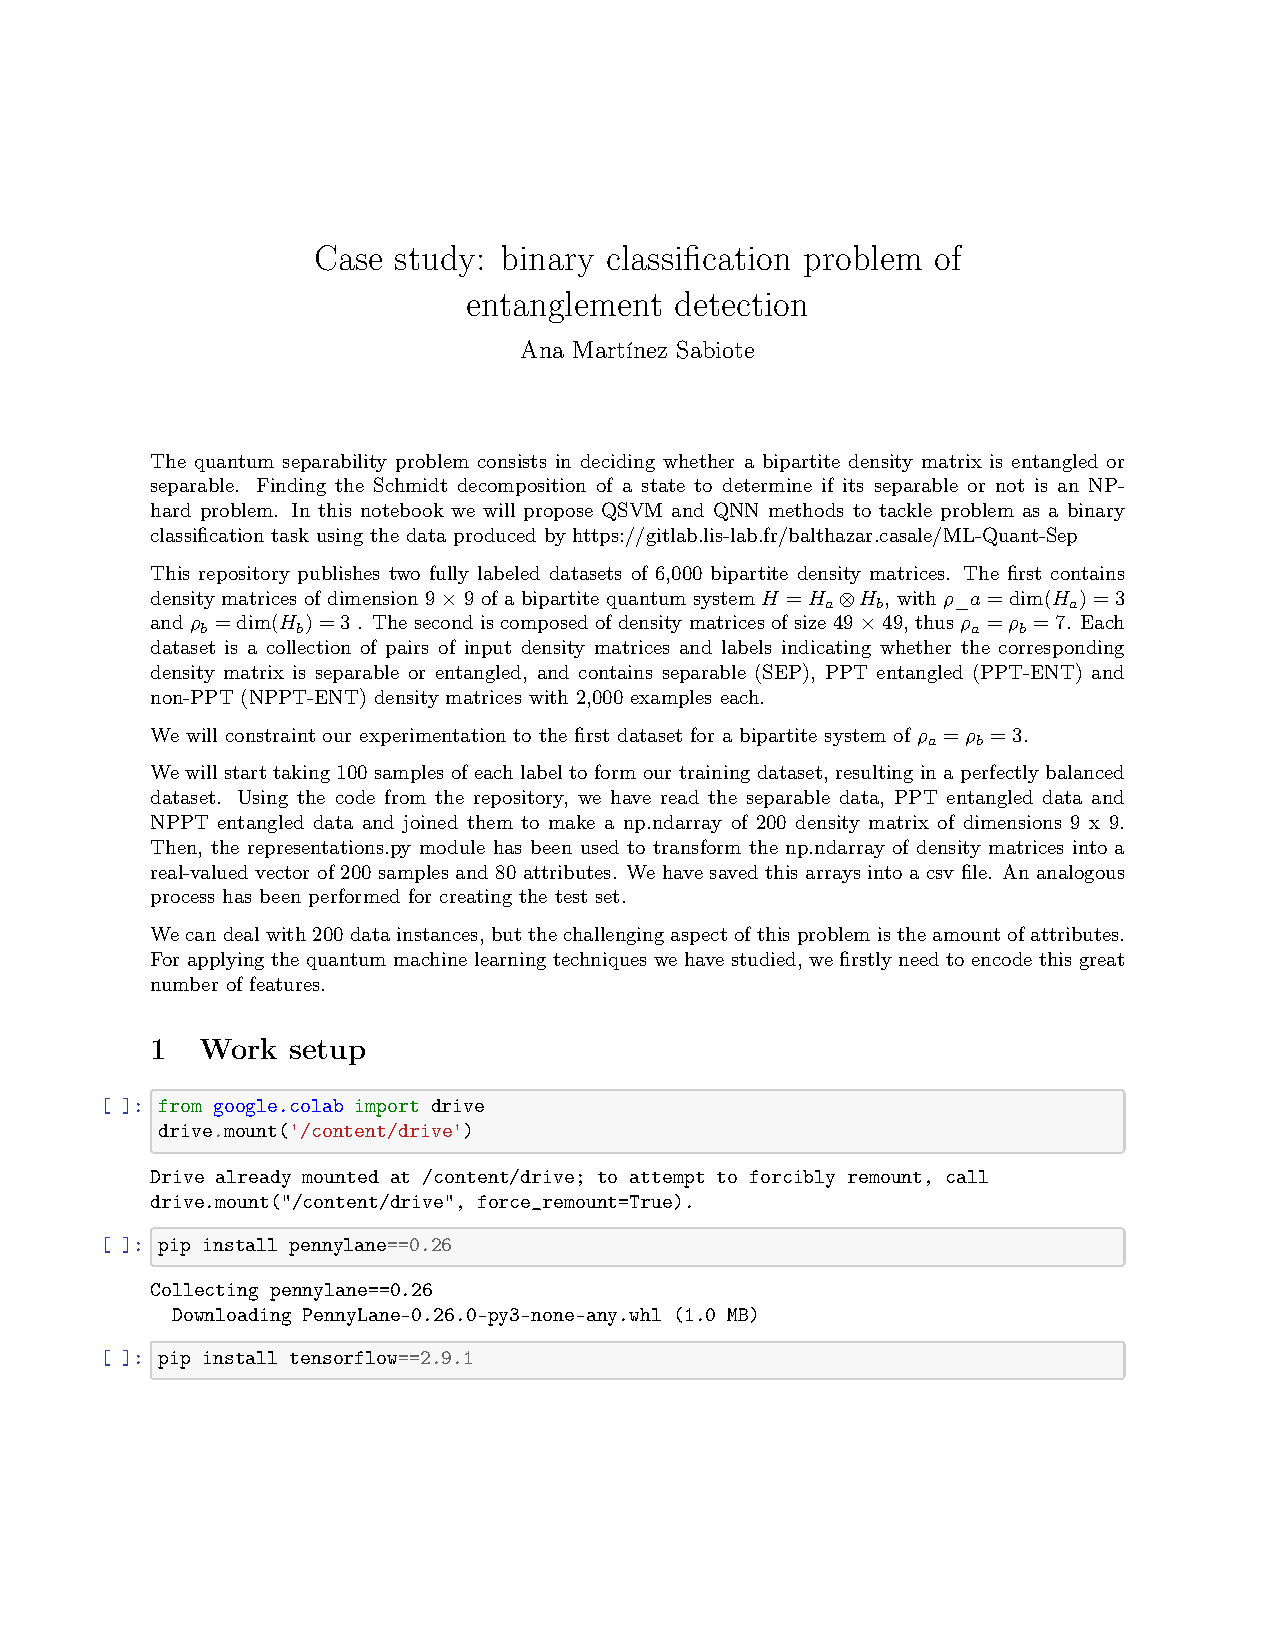
\includepdf[pages=-,pagecommand={},addtotoc={
	1,section,1,Work setup,p1,   
	2,section,1,Pre-work to get started,p2,
	37,section,1,Case study: dataset with 0.5 PPT ratio,p3,
	76,section,1,Case study: dataset with 1.0 PPT ratio,p4}]{apendices/notebook_appendix.pdf}

  
% Añadir tantos apéndices como sea necesario 

% -------------------------------------------------------------------
% GLOSARIO: Opcional
% -------------------------------------------------------------------



% -------------------------------------------------------------------
% BACKMATTER
% -------------------------------------------------------------------

\backmatter % Desactiva la numeración de los capítulos
\pdfbookmark[-1]{Referencias}{BM-Referencias}

% BIBLIOGRAFÍA
%-------------------------------------------------------------------

\bibliographystyle{alpha-es} 
\begin{small} 
  \bibliography{library.bib}
\end{small}


\end{document}
